\chapter{Reproducibility study}
\label{chap:reproducibility}

The following chapter describes a yet to be published collaboration with manuscript in preparation.
My contribution to this project was preparing the scripts to run the HOOMD simulations, writing documentation for the project, and involvement in numerous group discussions. 
This study brought to light many many issues which instigated many updates and improvements to the various codes used in the study.
Scientific software improvements I am responsible for as a result of this study include:
\begin{enumerate}
    \item Allow HOOMD functions to add to an existing snapshot to facilitate rigid bodies. \href{https://github.com/mosdef-hub/mbuild/pull/808}{(mBuild pull request \#808)}
    \item Ported the rigid body constraint class from the HOOMD v2 to v3 API. \href{https://github.com/glotzerlab/hoomd-blue/pull/888}{(HOOMD pull request \#888)}
    \item Allow \texttt{mBuild}'s xyz writer to write coordinates with greater precision, so MCCCS could use it for this study. \href{https://github.com/mosdef-hub/mbuild/pull/996}{(mBuild pull request \#948)}
    \item Added the required neighborlist buffer argument to the \texttt{mBuild} \lstinline{create_hoomd_forcefield} function to address breaking change in the HOOMD neighborlist API. \href{https://github.com/mosdef-hub/mbuild/pull/988}{(mBuild pull request \#988)}
    \item Fixed a bug in the conversion of Ryckaert-Belleman (RB) to OPLS-style dihedrals. \href{https://github.com/mosdef-hub/mbuild/pull/996}{(mBuild pull request \#996)}
    \item Corrected Coulomb's constant used in the charge conversion for HOOMD writers. \href{https://github.com/mosdef-hub/mbuild/pull/1011}{(mBuild pull request \#1011)}
    \item Add optional calculation of energy and pressure tail correction to the Lennard-Jones pair force. \href{https://github.com/glotzerlab/hoomd-blue/pull/1138}{(HOOMD pull request \#1138)}
\end{enumerate}

\section{Introduction}
%% background
Reproducibility in science means that we are transparent about our methods in a way that allows others to understand what was done.
If the goal of science is to expand the knowledge of humankind, making sure experiments are reproducible helps to lay a strong foundation for the next discovery.
In computational molecular simulation, where all parameters can be controlled, it would seem an easy task to reproduce an existing work.
Molecular dynamics (MD) and Monte Carlo (MC) simulation are both driven by the core principles of statistical thermodynamics.
Many codes for performing these methods exist each with their own algorithms and implementations, but if each code is correctly using the core principles, the end result should be the same.

This study aims to learn whether different codes can get the same result using the same model.
Within the umbrella of model is the thermodynamic ensemble (e.g., NVT, NPT), the representation of the system (e.g., the force field, constraints, cutoffs), and the statepoint (i.e., the pressure, temperature).
In this framework, a "force field" is defined to supply the parameters for a given model.
Other details related to the model are rigid representation and long-range and charged interactions.

In computational molecular simulation, already many hurdles to achieving simulation reproducibility have been reported. 
Using the same method, ensemble, and forcefield may not ensure reproducibility between engines, as different engines lack consistency in the functional forms, implementations, and options for handling long-range and charged interactions \citep{Rizzi2020}. 
The energy calculated with certain codes has been found to depend on how the charges are calculated (whether the charge method uses the whole molecule or fragment) and which charge calculation method is used is often not reported---even differences in Coulomb's constant may cause different results \citep{Shirts2017}.
Due to differences in available implementations in the difference engines there is no one size fits all protocol \citep{Loeffler2018}.
Systematic error was found between engines in as simple a task as calculating the potential energy and density of uncharged molecules in the liquid phase, even between groups using the same engine \citep{Schappals2017}.
Although these hurdles may seem discouraging and lead some to disregard simulation entirely, I would argue that instead this is a challenge that be met by the community using TRUE principles.

This study, a multi-university collaboration, aims to determine what information is necessary to achieve statistically same results across engines.
Researchers from eight universities (see \autoref{tab:unis}) contributed to scripts to initialize and run each of these systems.
\begin{table}[h!]
\caption{Universities participating in the study and their abbreviation.}\label{tab:unis}
\centering
\begin{tabular}{ll}
BSU & Boise State University \\
UD & University of Delaware \\
UH & University of Houston \\
UM & University of Michigan \\
UMN & University of Minnesota \\
UND & University of Notre Dame \\
VU & Vanderbilt University* \\
WSU & Wayne State University
\end{tabular}
\end{table}
Six different engines (see \autoref{tab:engines}) were used to conduct molecular dynamics (MD) and Monte Carlo (MC) simulations.
\begin{table}[h!]
\caption{Simulation engines used in the study along with the publications in which the engine is described, simulation type, and the research group responsible for that engine.}\label{tab:engines}
\centering
\begin{tabular}{llll}
Code      & Type & Ref             & Group   \\ \hline
Cassandra & MC   & \cite{Shah2017} & UND     \\
GOMC      & MC   & \cite{Shah2017} & WSU     \\
Gromacs   & MD   & \cite{ABRAHAM201519, Pall2015, Smith2013, Lindahl2001, BERENDSEN199543, https://doi.org/10.1002/jcc.20291, Hess2008} & VU      \\
HOOMD     & MD   & \cite{Anderson2020, Nguyen2011a, Glaser2020a, Lebard2012} & BSU, UM \\
LAMMPS    & MD   & \cite{LAMMPS} & UD, VU  \\
MCCCS     & MC   & \cite{C8SC05340E,Josephson2019} & UMN    
\end{tabular}
\end{table}
These scripts will use tools from the Molecular Simulation and Design Framework (MoSDeF) to help with reproducible simulation initialization.
In order to help manage this large data space and submission to various clusters, the \texttt{signac} framework will be used to programmatically organize the statepoint directories and handle the idiosyncrasies of different cluster schedulers.
This study is still ongoing, so some of the data shown in this chapter may be unfinished or incomplete. 
I will focus most on the simulations run using HOOMD, as this is the part of the study I am responsible for.
I will also try to distill what we have learned, through the numerous issues we have discovered and overcome. 
This project involved a great deal of collaboration and discussion.
Although the systems studied are very simple, we ran into many challenges:
Keeping consistent units, sharing data, and overcoming the many unexpected hurdles to get consistency between engines due to the different available functions in each engine. % wording?
In addition, choosing what information to store and how to format that information so it is readable by one analysis script was challenging between multiple engines because not all engines were able to report the same values.
The benefit of this study is that it provides comprehensive information: the results obtained and the exact code ran to obtain them. 
These data can be used by other simulators to validate their work.
These workflows can also serve as valuable examples. 
At the time this study started, HOOMD v3 was still in beta, so the HOOMD part of this project can serve as a valuable example of how to (1) run atomistic simulations consistently with other engines, (2) initialize rigid bodies and bond constraints using the MoSDeF framework (this workflow is currently the only available example of how to initialize rigid bodies on an existing system), and (4) log individual energies such that they can be compared to other engines. 
We have learned that even when you control every step of the initialization process, there are still so many additional user-tuned parameters in each engine that guaranteeing reproducibility requires careful thought.

\section{Models}

The systems which are studied are small, simple, and chosen to demonstrate simulation in systems with varied degrees of complexity:
\begin{figure}[h!]
    \centering
    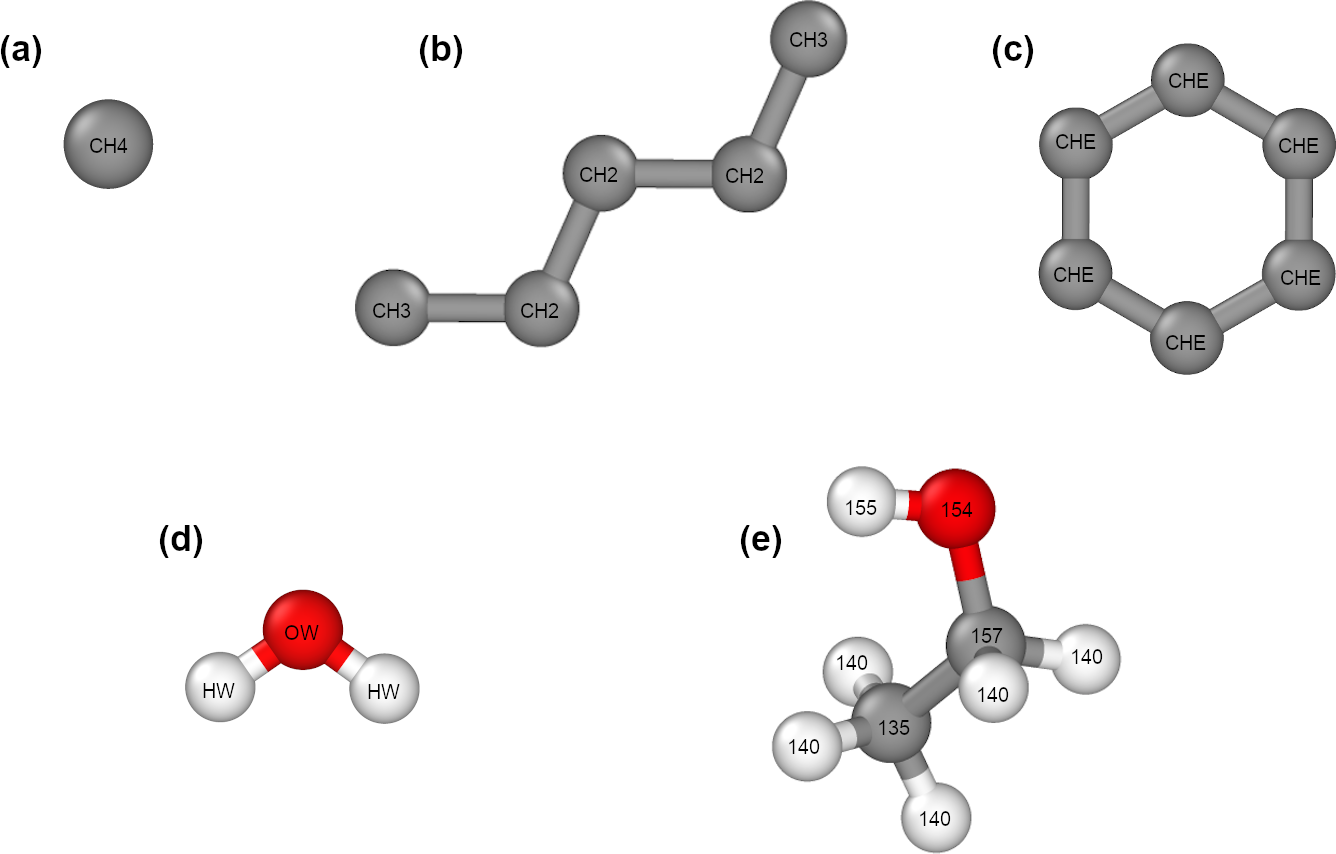
\includegraphics[width=\linewidth]{figures/rep_study/models.png}
    \caption{Structures of the five models with the atoms types labelled: (a) TraPPE-UA methane, (b) TraPPE-UA pentane, (c) TraPPE-UA benzene, (d) SPC/E water, (e) OPLS-AA ethanol}\label{fig:models}
\end{figure}
The TraPPE united-atom (UA) forcefield was applied to UA methane (see \autoref{fig:models}a) and pentane (see \autoref{fig:models}b) models to investigate the simplest case of only Lennard-Jones interactions and a linear molecule with bonds, angles and dihedrals \citep{Martin1998}.
TraPPE-UA was also applied to a UA benzene model (see \autoref{fig:models}c) to investigate rigid ring structures.
(We initially tried a flexible model based on TraPPE-UA, but some engines were not able to get this model to run \citep{Yiannourakou2019}.)
The SPC/E water model (see \autoref{fig:models}d) was used to investigate a rigid molecule with electrostatics \citep{Berendsen1987a}.
Finally, the most complex system, the OPLS all-atom (AA) forcefield was applied to ethanol (see \autoref{fig:models}e) to investigate a fully atomistic, charged molecule \citep{Jorgensen1988}.
The step-wise, increasing complexity in these systems was later very useful for pinpointing the source of a discrepancy between engines.

The nonbonded interactions were modelled as Lennard-Jones (LJ) interactions with long-range correction to energy and pressure. (This correction is discussed further in \autoref{sec:cutoff}.)
And charged interactions are computed via the particle particle particle mesh (PPPM) method as described in \citet{Darden1993} and \citet{Lebard2012}. 
The bonded interactions were modelled as harmonic bonds, harmonic angles, and OPLS style dihedrals.
The forcefield parameters for TraPPE-UA and OPLS-AA are provided with \texttt{foyer} \citep{foyer}. 
The non-bonded potential parameters for SPC/E water can be found in \autoref{tab:water}. 
The non-bonded TraPPE-UA potential parameters used for benzene can be found in \autoref{tab:bz_nonbond}. No bonded potentials were used for either water or benzene as both molecules were modelled as a rigid bodies \citep{Nguyen2011a, Glaser2020a}. 

\section{Methods}

The scope of this project meant that it required thoughtful organization: A total of sixty-nine statepoints each in sixteen replicates were distributed to eight different universities.
Devising a custom organization scheme would've been time-consuming and potentially unreliable, so the parameter space was handled by the \texttt{signac} framework\cite{Adorf2018, signac_zenodo, signac_scipy_2018, signac_scipy_2021}.
\texttt{Signac} is a tool designed for managing dynamic data spaces in a well-defined, indexable way.
The study is formatted as a \texttt{signac} project, so all code---from system initialization to project analysis for all engines---is contained in a single repository, and access to the data, or "job", can be done using the statepoint parameters.

The workflow for the HOOMD simulations in shown in \autoref{fig:rep_workflow}; each engine will have similar although perhaps not identical workflows.
\begin{figure}[h!]
    \centering
    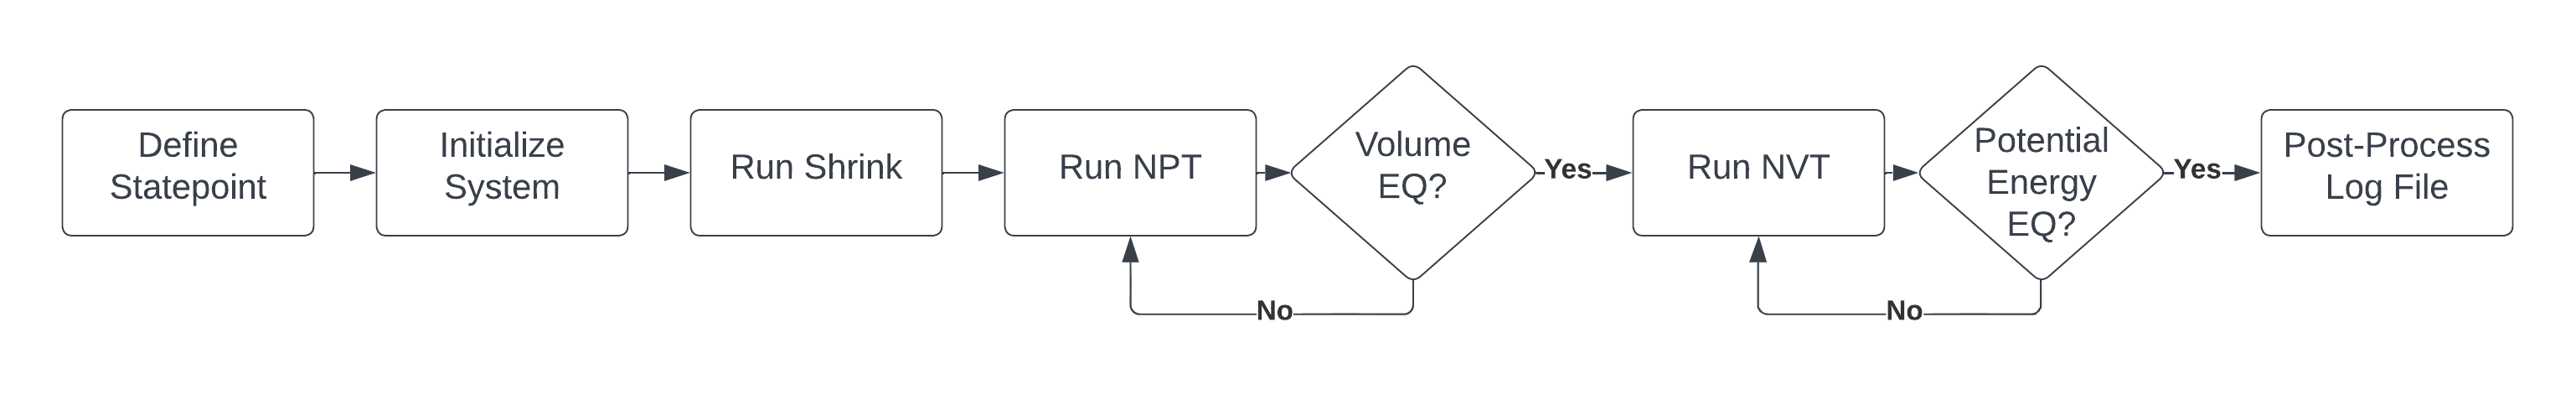
\includegraphics[width=\linewidth,keepaspectratio]{figures/rep_study/reproducibility_workflow.png}
    \caption{Workflow for HOOMD simulations in the reproducibility study.}\label{fig:rep_workflow}
\end{figure}
First the statepoint data is used to define the job: The statepoint definition consists of the molecule being simulated, the temperature and pressure at which the simulation is run, the simulation ensemble, the number of molecules (N), the side length of the cubic box, the target density, the molecule mass, the forcefield, including the cutoff style and cutoff distance ($r_{cut}$), and the engine used to simulate that statepoint. 
To provide adequate data for statistical analysis, 16 replicates were run at each statepoint.
Then using the statepoint data, the system (including the starting structure, box, etc.) is initialized programmatically.

To ensure that all engines are starting with the same system, this process is generalized: All engines use the \lstinline{construct_system} function, which wraps \texttt{mBuild}'s \lstinline{fill_box} to creates an \texttt{mBuild} \lstinline{Compound} object containing the simulation box at the specified density populated with the specified number of molecules, and \lstinline{load_ff}, which loads the correct \texttt{foyer} \lstinline{Forcefield} object from the forcefield name in the statepoint. 
Then the forcefield is applied to the system box compound to generate a ParmEd structure\cite{Shirts2017}, where the atoms are typed according to the forcefield and the relevant force parameters are also stored within the structure object. 
From there each engine takes the parameterized ParmEd structure and converts it to the necessary input format. 
For HOOMD this is done using the \lstinline{create_hoomd_forcefield} function in \texttt{mBuild}, which handles the unit scaling, initial snapshot creation, and neighborlist and force creation using the information stored in the ParmEd structure. 
Some adjustments are made to the snapshot and forcefield after this to handle rigid bodies, constrained bonds, neighborlist exclusions, and long range correction. 
Then the simulation is initialized, the integrators, methods, and logging are set and the simulation can be run. 

The first run step in this process is to run a brief shrink step to bring the system to the desired density. 
The shrink step starts with the volume expanded by 8 times (each length of the target box is 2 times larger) then the box is shrunk in the NVT ensemble over 100 ps with a thermostat coupling value of 1 ps at the simulation temperature. 
The NPT run is initialized from the final frame of the shrink trajectory and is run at high thermostat (1 ps) and barostat (5 ps) coupling values initially (for the first 1 ns) to prevent large fluctuations in the pressure and kinetic temperature and then they are lowered (to 0.1 ps and 1 ps, respectively) for the duration of the run. %(Initial tau=1000dt tauS=5000dt for 1e6 steps then tauS=1000dt tau=100dt for 5e6 steps.) 
The NPT ensemble is run for a minimum of 6 ns, but after each NPT run, pymbar's \lstinline{detectEquilibration} and \lstinline{subsampleCorrelatedData} functions are used to check whether the volume has equilibrated and the desired number of decorrelated samples have been run \cite{Chodera2007, Chodera2016, Shirts2008a}. 
A minimum of 100 independent samples at equilibrium were collected for each run, and this equilibration detection and subsampling is applied across all engines.
By using a quantitative metric to achieve the same number of equilibrated, decorrelated samples, as opposed to deciding whether a simulation is equilibrated by eye or running for an arbitrary time, we aim to reduce user error in our sampling.
Plots of the evolution of potential energy over time for the simplest (UA methane) and the most complex system (AA ethanol) can be found in \autoref{fig:methane_pe_evolution} and \autoref{fig:ethanol_pe_evolution}.
If the volume has not equilibrated or the minimum number of independent samples have not been run, then the NPT simulation continues at the lower thermostat and barostat coupling values for an additional 5 ns. 
If the volume has equilibrated, then the statistically independent samples of the equilibrated volume are averaged and this average is logged to the job document and the job moves to the NVT run. 
The NVT run is initialized from the final frame of the NPT trajectory, but because this final frame may not be at the average volume, a short (20 ps) shrink period is done for the initial NVT run and then the simulation is run for 5 ns. 
After the NVT run, the same equilibration detection is used---this time looking at the potential energy values. If the potential energy is equilibrated, the NVT run is finished, otherwise it is run again for an additional 5 ns from the last frame of the proceeding NVT run. 

Finally the log file containing thermodynamic information written out by HOOMD is processed to remove any extra headers within the data from restarted jobs, the pressure and temperature are converted from simulation units into kPa and K, and the density values are calculated from the volume and logged.
For each engine, the final step is to convert its log and trajectory files to a standard format and unit to allow analysis to run over all jobs.

All scripts used to initialize, simulate, and analyze this project are publicly available on GitHub \citep{reproducibility}.
To share the large data workspace between universities, the workspace folder is uploaded to a shared Dropbox using Rclone. 
Once the study is finalized the complete data will be distributed using Zenodo.
Along the way to achieving consensus between engines in this main project, many stumbling blocks were encountered. 
The following sections will detail the issues we encountered and their resolution.

\section{Single point energy comparisons}

In general when trying to achieve "correctness" in a complex system, it is advisable to first validate that correctness can be achieved in a simple system, then incrementally add complexity.
In this study, single point energy calculations were done after discrepancies were found in the simulation results.
With the benefit of hindsight, it is clear that starting with a single point energy comparison would've been much more efficient---allowing discovery of many issues early in the study before numerous compute hours were consumed. 
It is a good rule of thumb for simulators to provide a snapshot along with its energy breakdown when publishing if they want to aid reproduction of their work.

The single point energy evaluation involved distributing the complete information for the starting system: atom coordinates and bonding and box information. 
The reason this starting structure needed to be distributed is because it was necessary to ensure all starting structures were identical:
The packing functions in \texttt{mBuild}, including \lstinline{fill_box} which was used to create the initial simulation inputs for this study, are wrappers for PACKMOL \citep{Martinez2003, Martinez2009}.
PACKMOL uses an intrinsic random number generation method which is compiler dependent. 
The result is that PACKMOL creates different systems based on the operating system on which it was compiled.
In general, simulators are interested in comparing a sampling of the equilibrium ensemble, which should not depend on the initial position.
However, this discrepancy is important to note if one is trying to compare the energies of a single frame!
For this reason, we could not rely on programmatically generated structures to compare the single point energies and it is good practice to distribute the input structure along with the code used to generate it.
This starting system was then initialized following the same procedure as the NPT/NVT ensemble simulations, but the simulation was not allowed to progress in time allowing direct comparison of the energies between engines.

Through the single point energy comparisons, it was determined that information about the 1-4 scaling and the combining rule were getting lost in the translation from \texttt{foyer} forcefield to ParmEd structure to engine input for Cassandra and Gromacs.
These errors were fixed by \texttt{mBuild} PR 1004 and 1010.
Initial comparison of the single point energies also showed large disagreement between the electrostatic energies of water in HOOMD and other engines. 
In HOOMD water was modelled as a rigid body. 
When the "rigid" neighborlist exclusion was added on to the default exclusions set by \lstinline{create_hoomd_forcefield} ("bond" and "1-3"), it was found that the exclusions were double counted by the PPPM energy calculation resulting in a large discrepancy in the electrostatic energy.
This is now noted in HOOMD's rigid body documentation.
Comparison of the single point energy calculations also helped to tune the grid size needed for HOOMD's PPPM charge calculation. 

The single point energy values after applying the fixes discussed are included in \autoref{tab:sp_methane}-\autoref{tab:sp_ethanol}, and in general these values were found to agree with some noted discrepancies:
Some engines are not able to report as thorough of a breakdown for energies or they may partition the energies differently.
For example, the long range and short range electrostatic energies are not the same between any engines; however, the total electrostatic energy is comparable.
By first validating our method using comparison of the single point energies, we were able to move into more complex simulations with greater confidence.

\section{Sensitivity of model to timestep}

Designing a general simulation workflow to work with the range of systems in this study required some model specific adjustments.
For example, the atomistic ethanol system required a smaller timestep.
When a timestep which was too large but small enough that the system didn't explode (i.e., the position update didn't push the particle outside of the simulation box) was used, the kinetic temperature was found to equilibrate to a lower value than was set in the NVT/NPT thermostat.
Unlike the other systems studied, ethanol has explicit hydrogens with harmonic bonds. 
Because hydrogen is such a light particle, the oscillations of bonds involving hydrogen are very fast.
(The SPC/E water system also has explicit hydrogens, but because it is rigid, the hydrogen bonds do not have these fast oscillations.) 

The temperature could not equilibrate to the set temperature because the timestep did not allow adequate sampling of the harmonic bond.
Consider the following example:
The period of the harmonic bond is given by
\begin{equation}\label{eq:harmonic_period}
    T = \frac{2\pi}{\sqrt{\frac{k}{m}}}
\end{equation}
where k is the potential constant for the bond given in the forcefield and m is the mass of the particle.
Initially, I was using a timestep of 0.001 (in simulation time units, approximately 1 fs when converted to real units) while the period of the harmonic bond (see \autoref{eq:harmonic_period}) was 0.0118 (in simulation time units, approximately 11 fs). \autoref{fig:harmonic_bond} illustrates the sensitivity of the harmonic bond sampled at different timesteps.
\begin{figure}[h!]
    \centering
    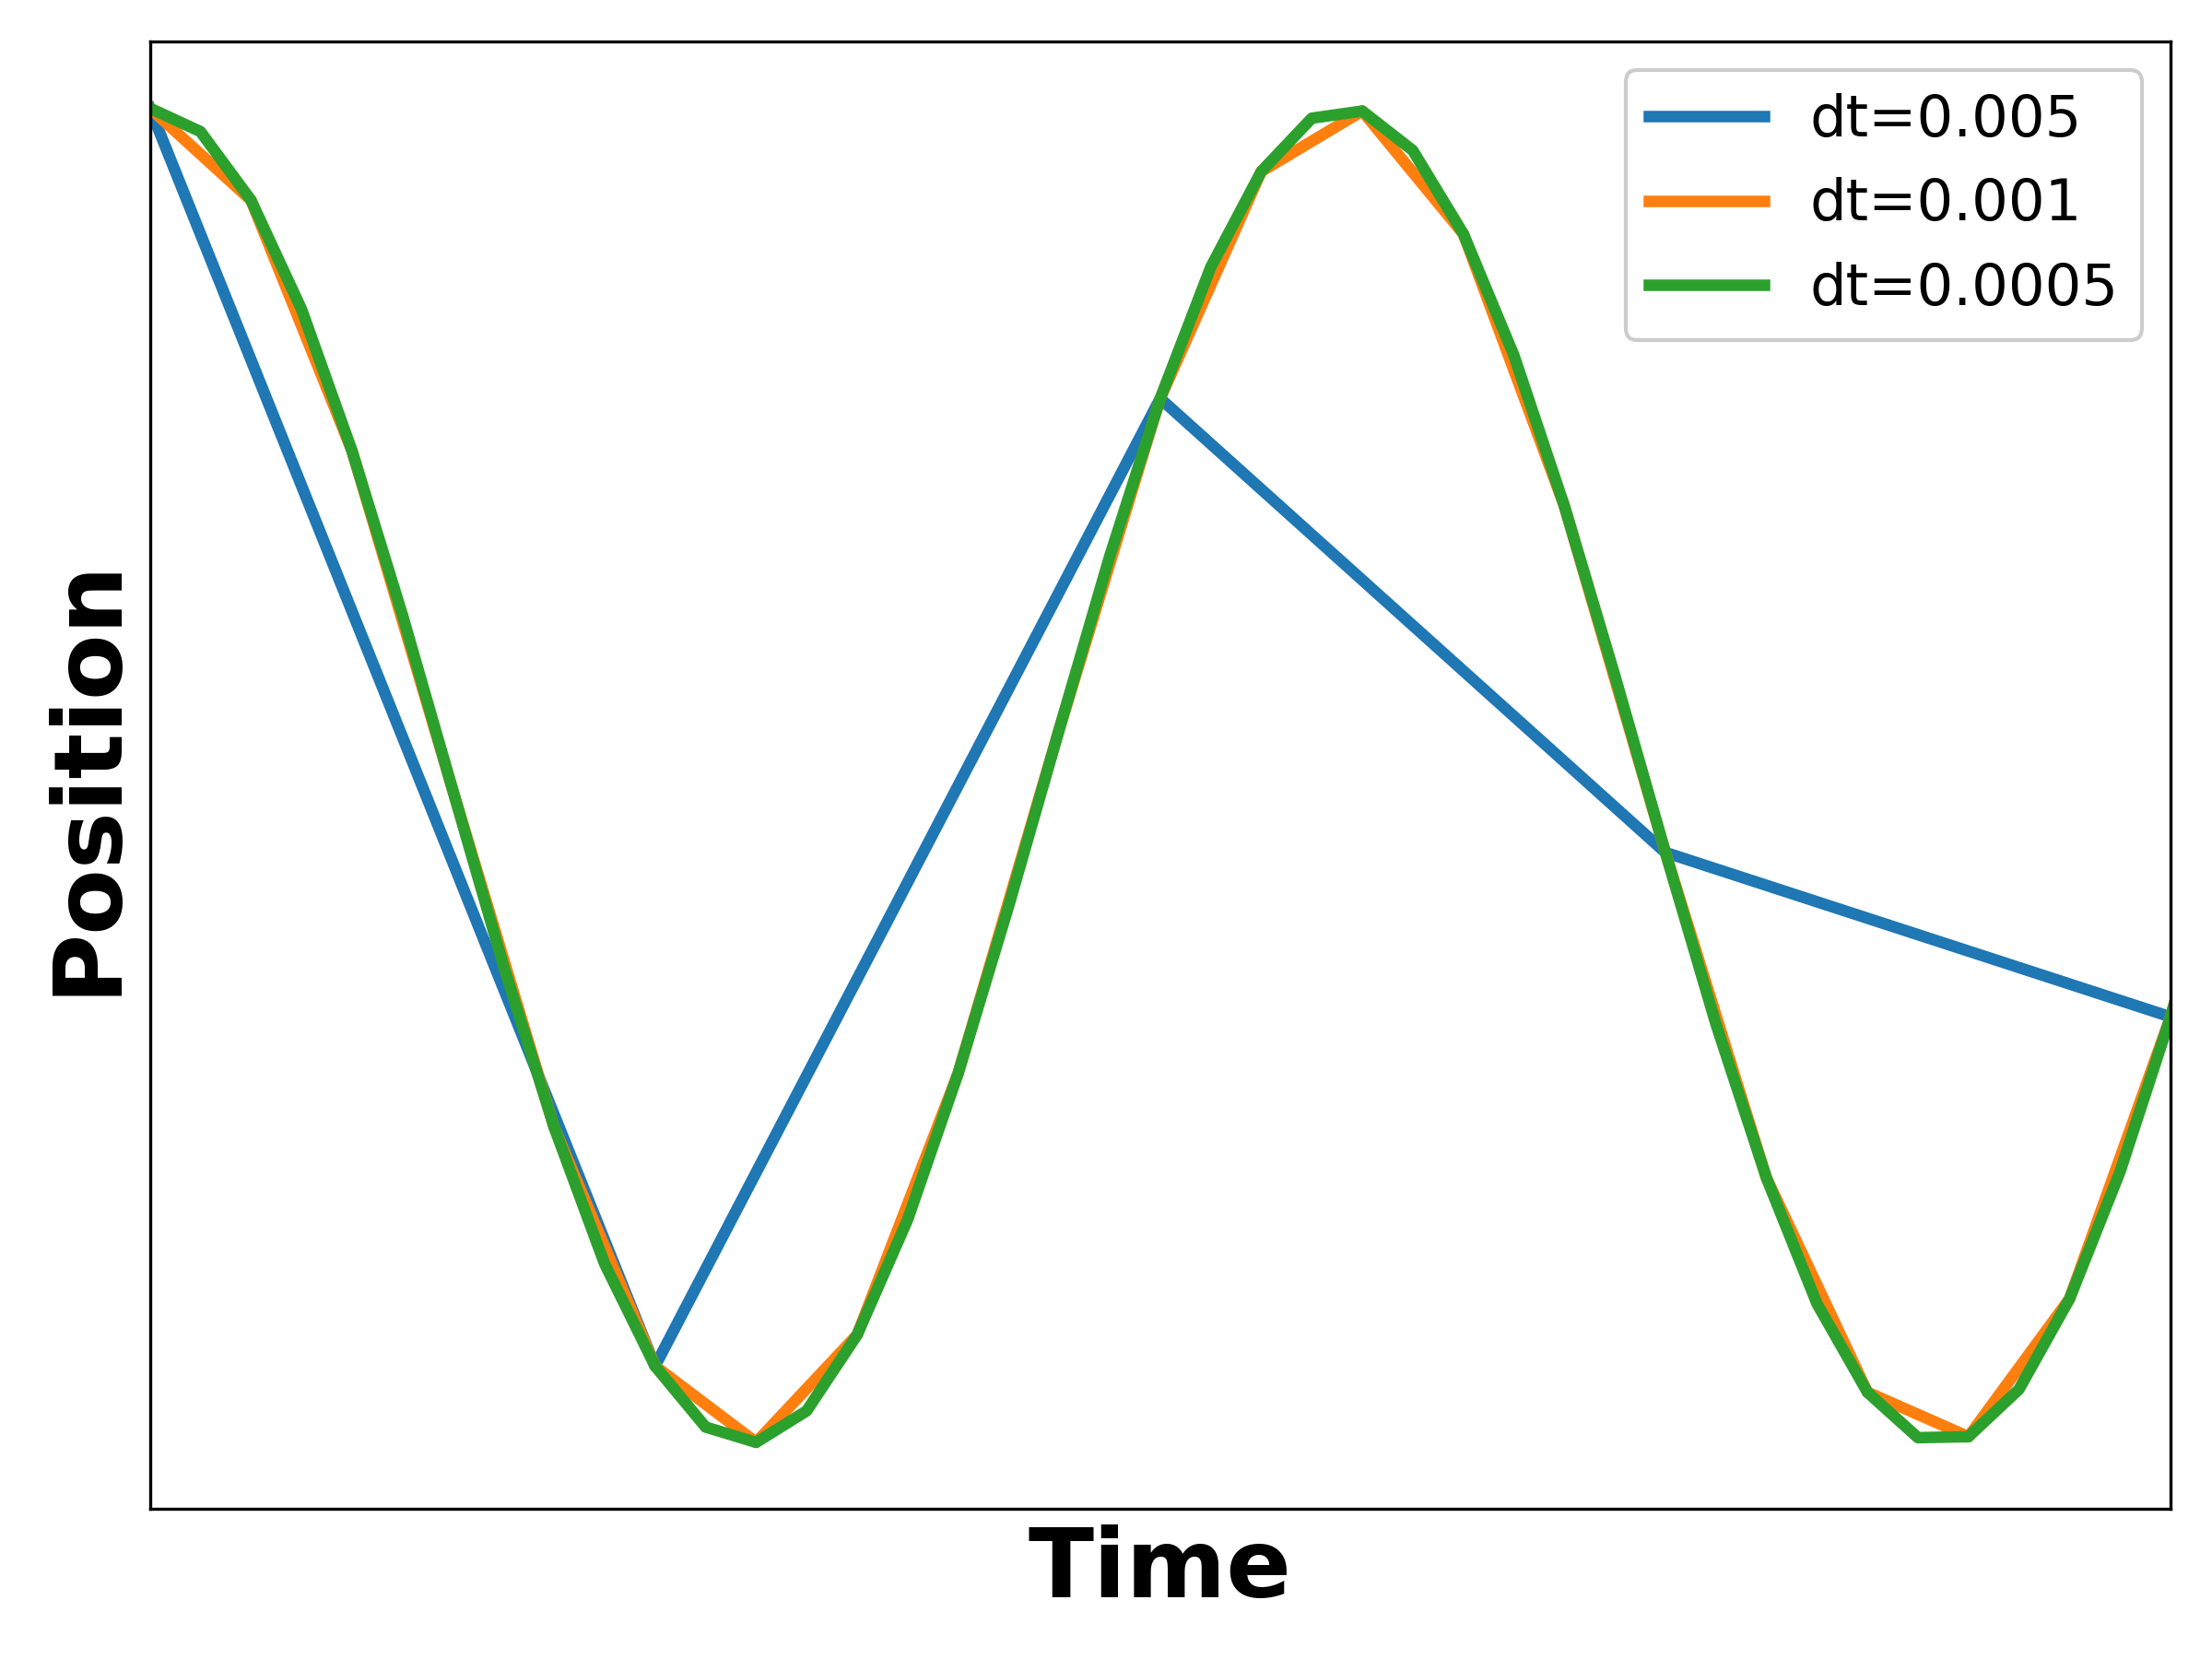
\includegraphics[width=0.6\linewidth,keepaspectratio]{figures/rep_study/harmonic_bond.png}
    \caption{Demonstration of how choosing too large a timestep can lead to poor sampling of the position of atoms in a harmonic bond. Note the divergence from sinusoidal as dt increases. The dt values and the harmonic bond equation are accurate with the values given for the hydrogen bond.}\label{fig:harmonic_bond}
\end{figure}
By using a smaller timestep (0.0005 in simulation time units, approximately 0.5 fs), the temperature equilibrated to the correct value.
\begin{figure}[h!]
    \centering
    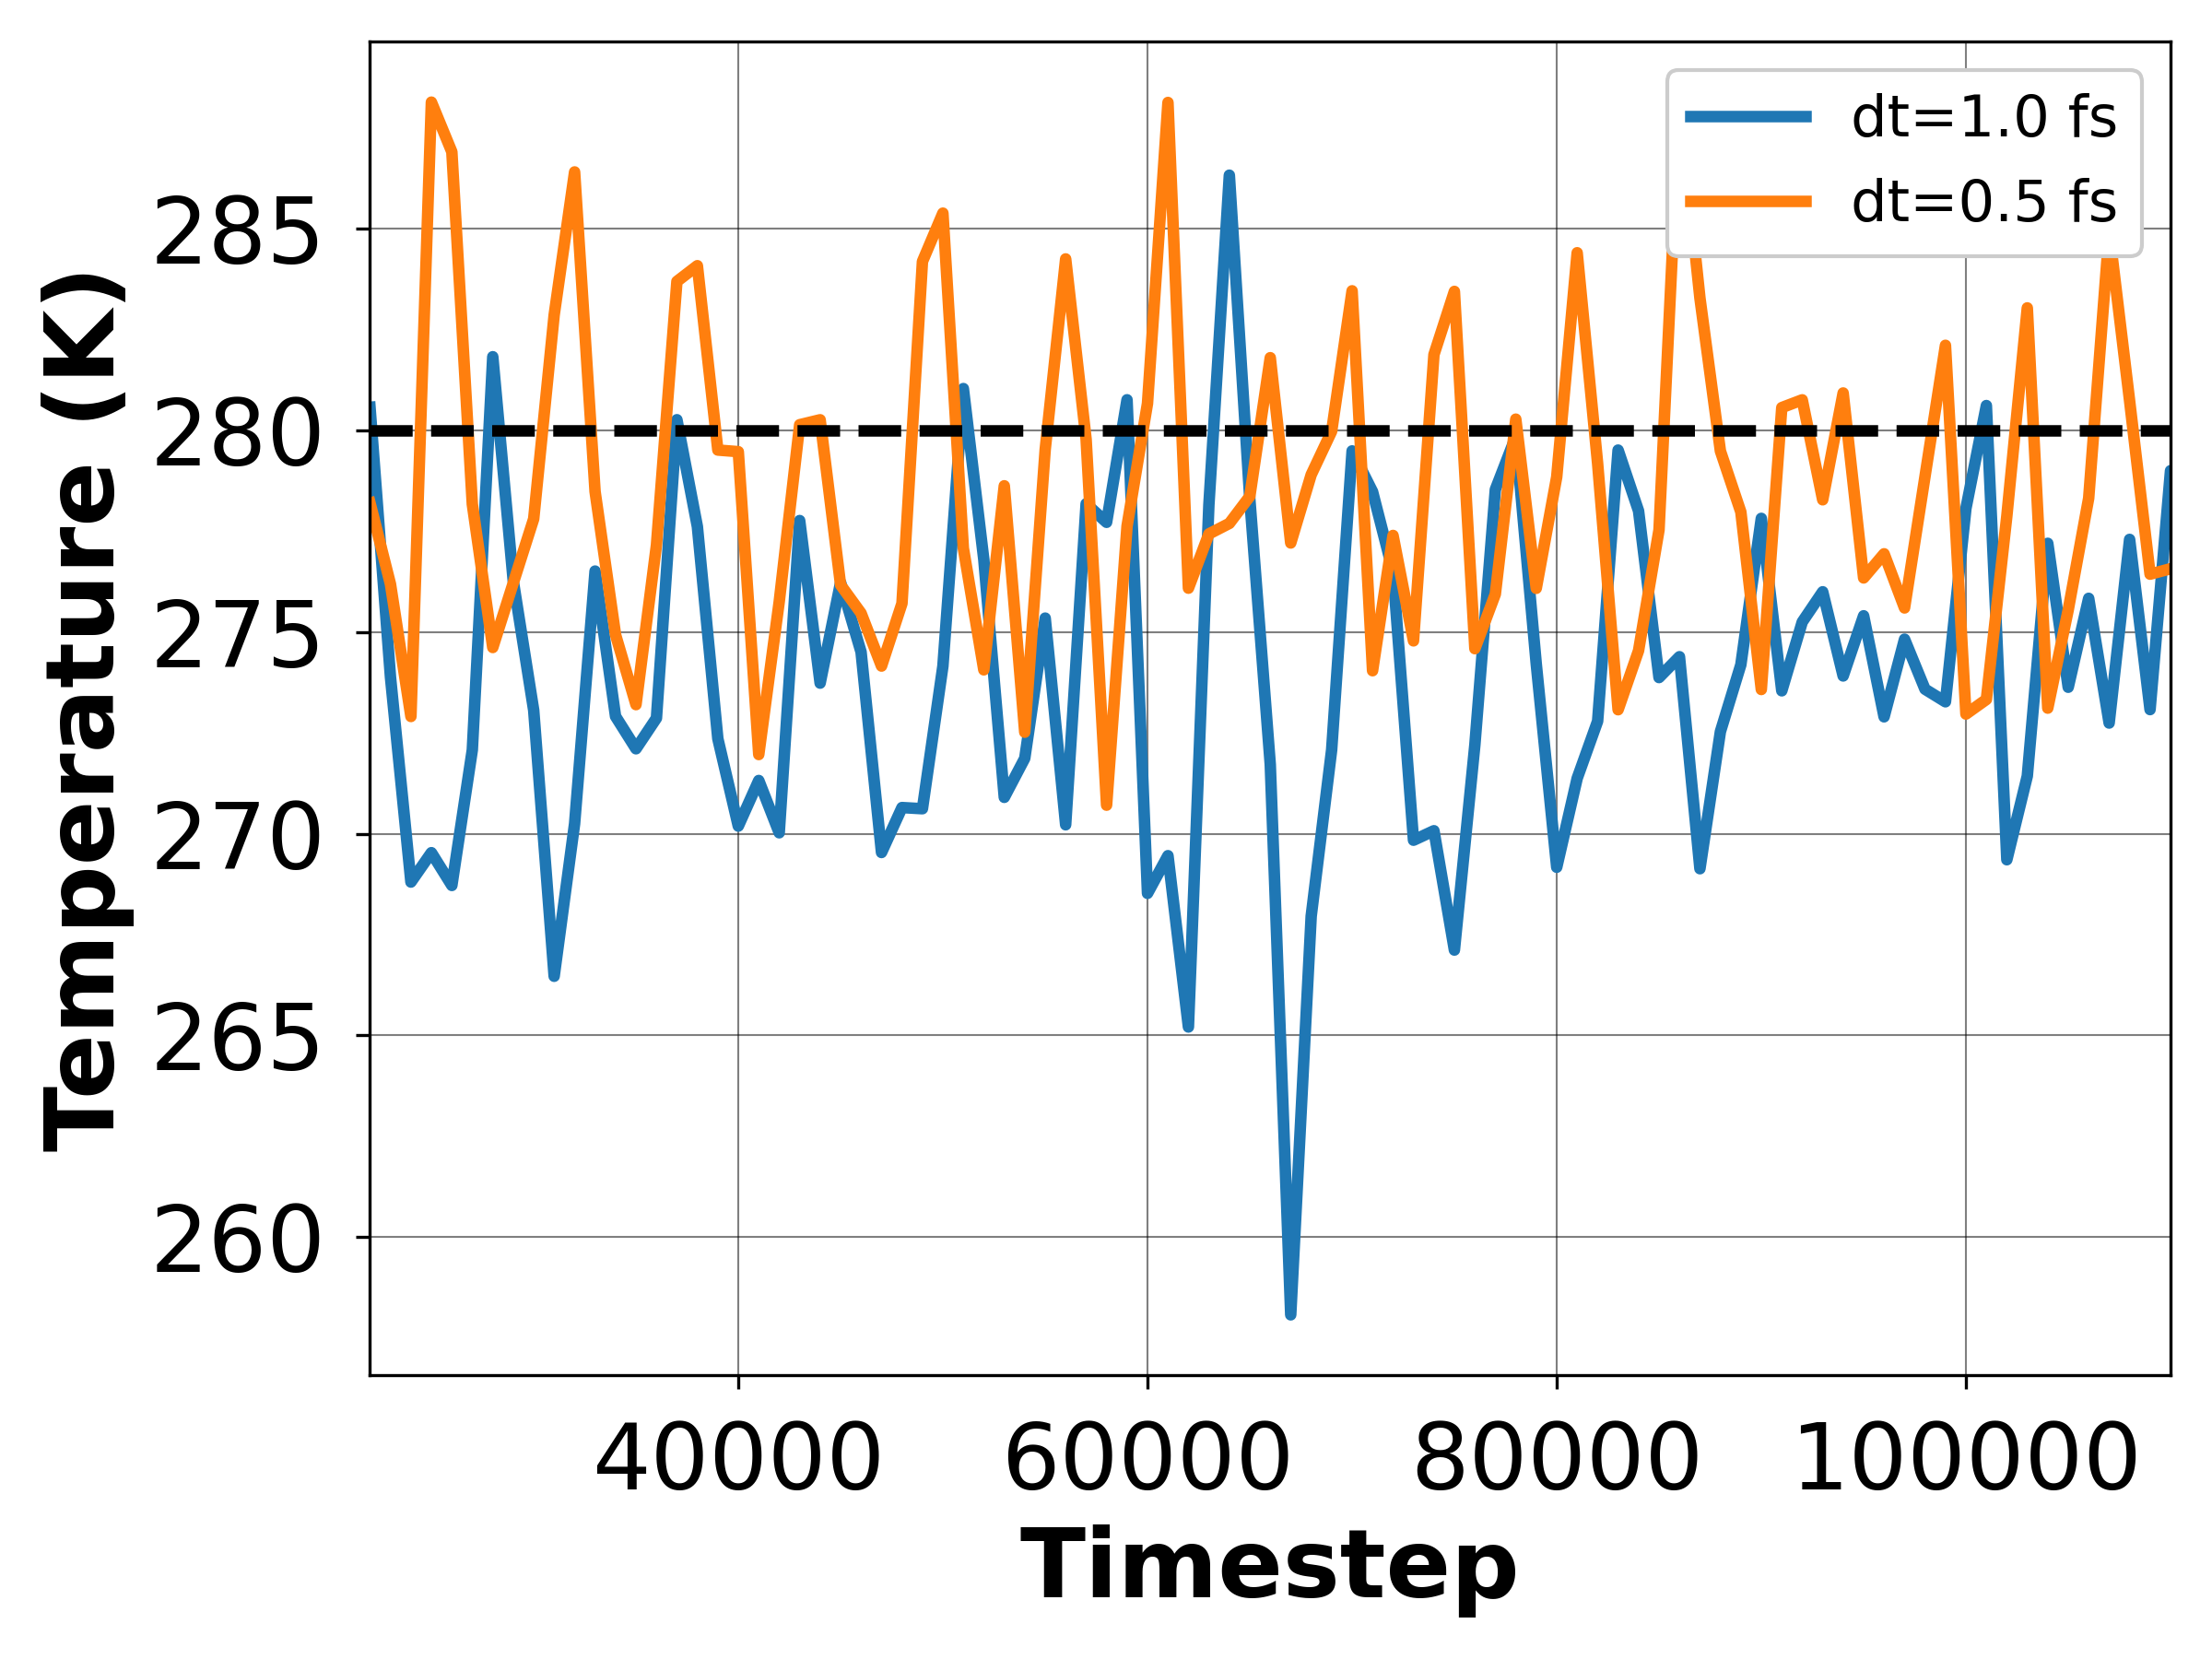
\includegraphics[width=0.6\linewidth,keepaspectratio]{figures/rep_study/temp_evolution.png}
    \caption{The evolution of temperature with time with the larger (1 fs) and a more reasonable (0.5 fs) timestep for the ethanol-AA system. The set temperature is shown as a dashed line. }\label{fig:temp_evo_ethanol}
\end{figure}
\begin{figure}[h!]
    \centering
    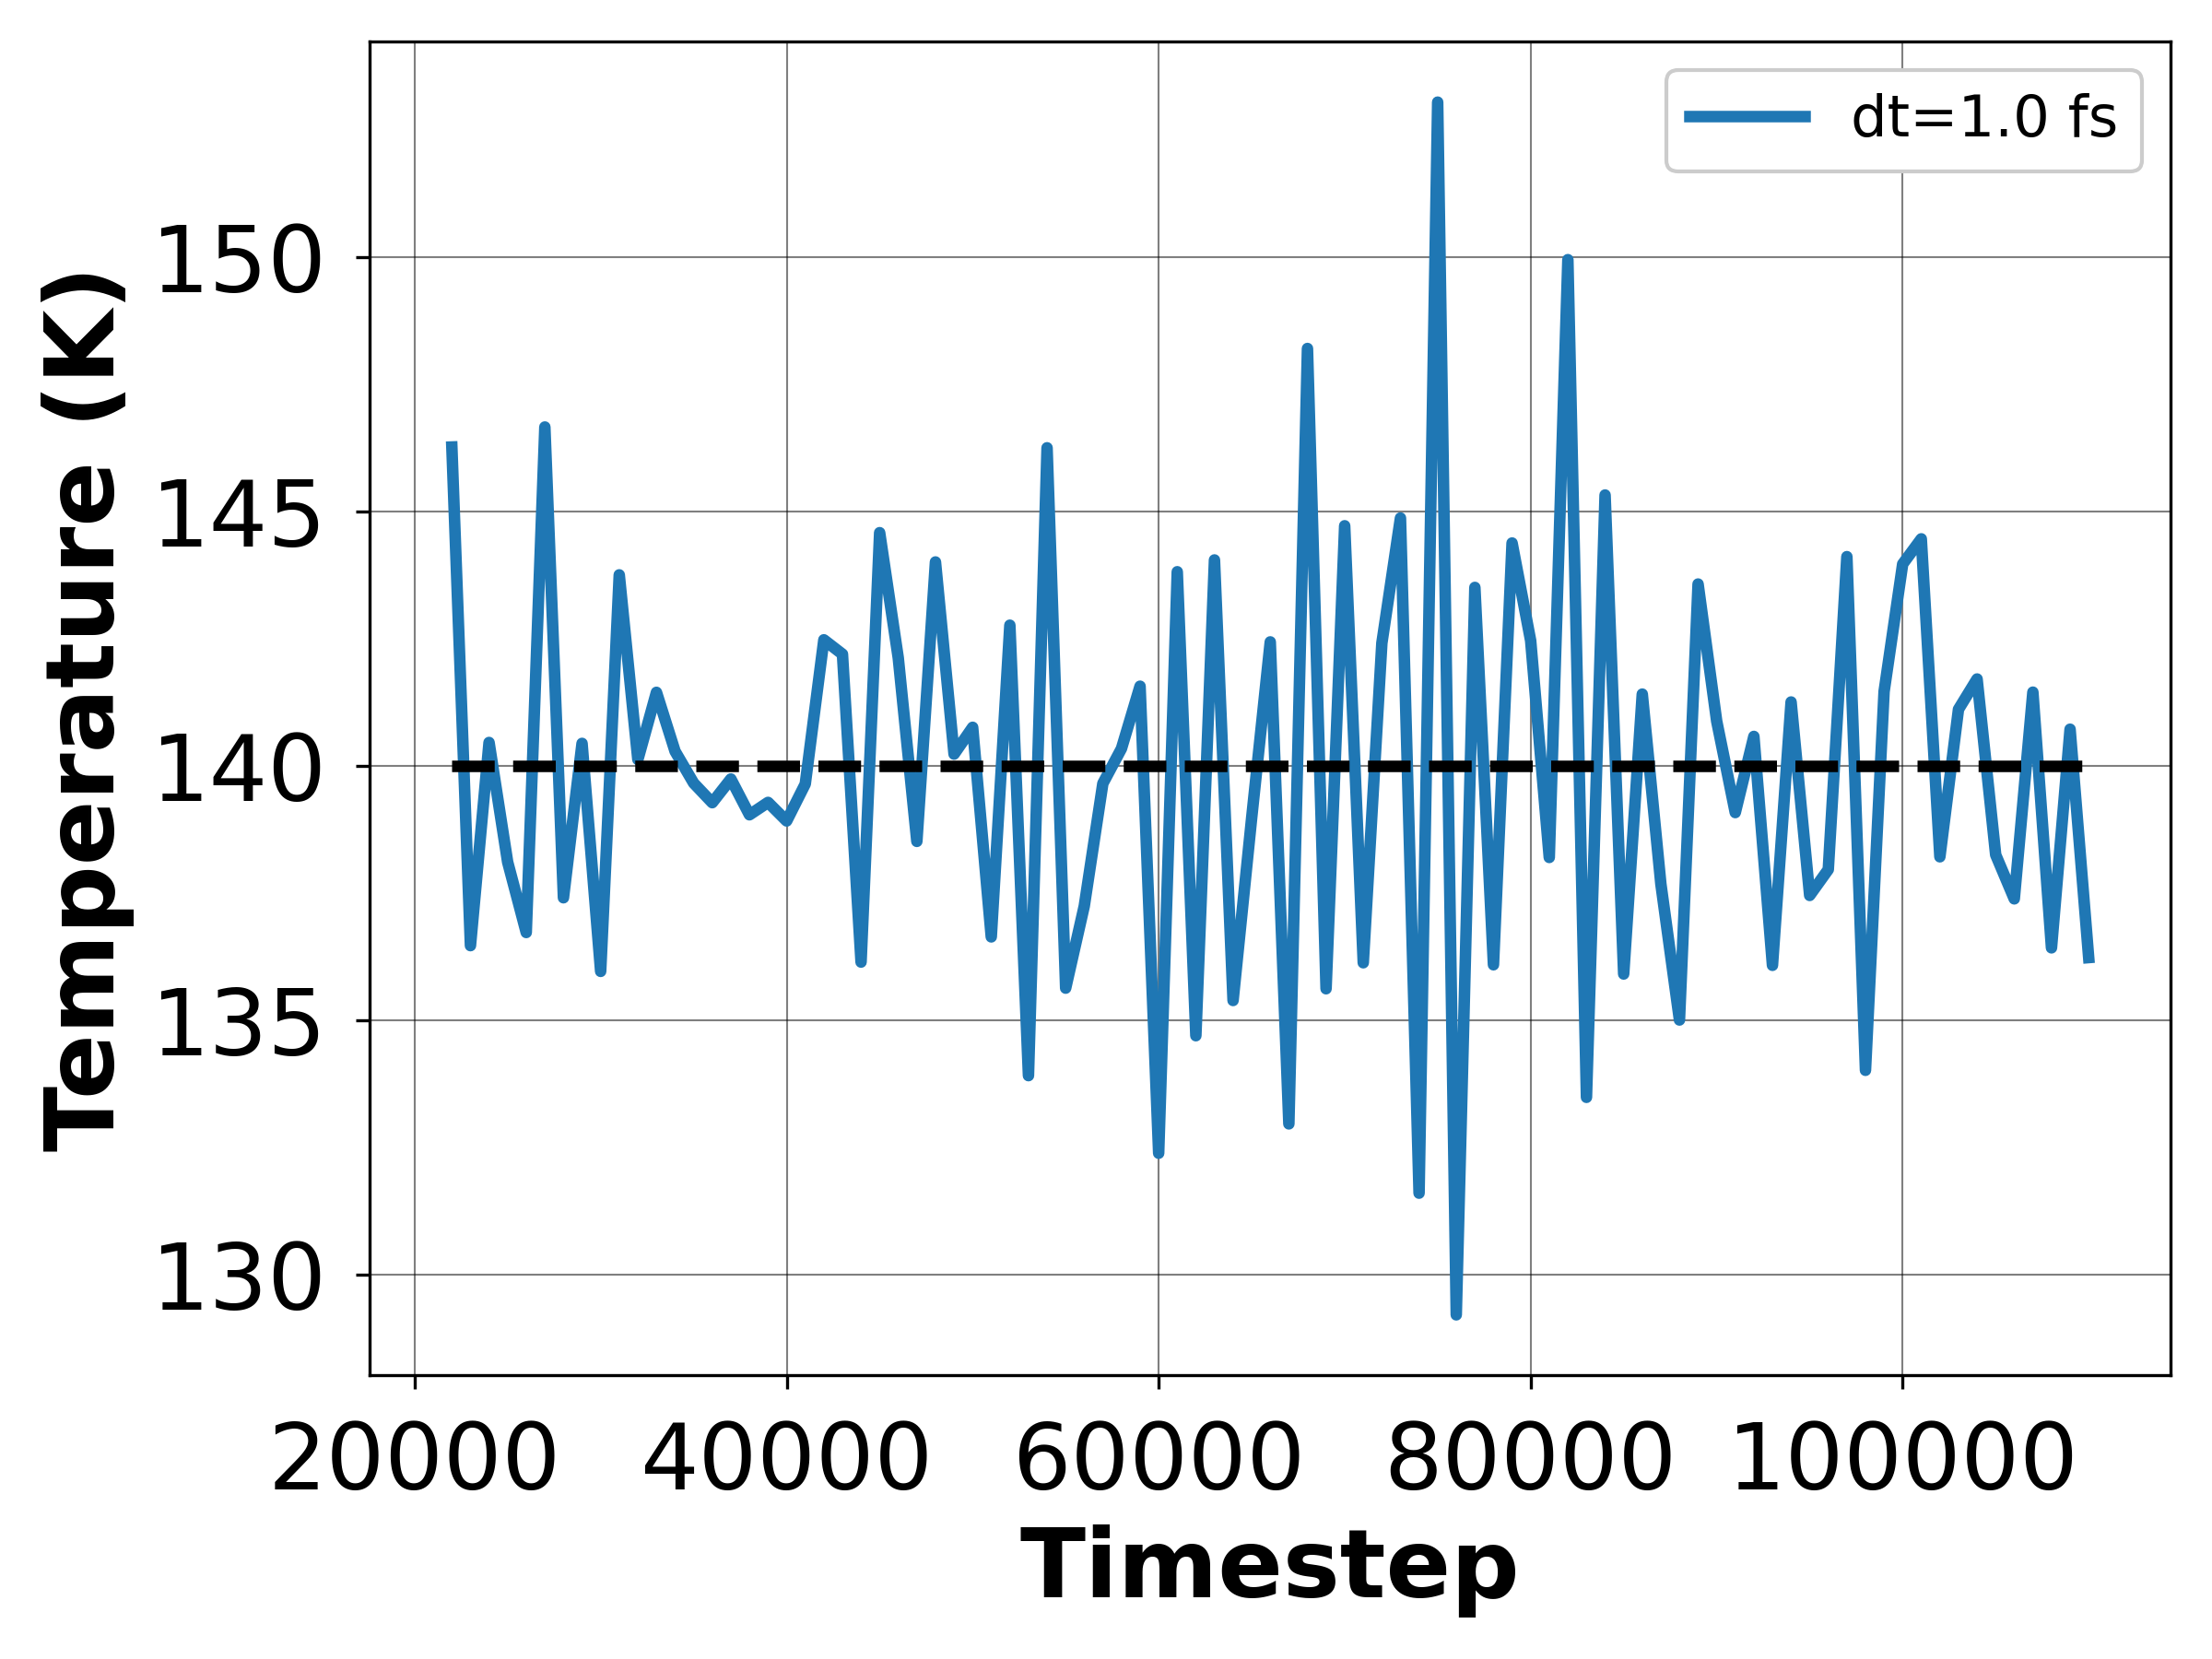
\includegraphics[width=0.6\linewidth,keepaspectratio]{figures/rep_study/temp_evolution_methane.png}
    \caption{The evolution of temperature with time with the larger (1 fs) timestep for the methane-UA system. The set temperature is shown as a dashed line.}\label{fig:temp_evo_methane}
\end{figure}
\autoref{fig:temp_evo_ethanol} and \autoref{fig:temp_evo_methane} show the sensitivity of the equilibrium temperature to timestep based on system complexity. 
Both plots are very noisy because they show only the initial 100 ps post-shrink equilibration in the NVT ensemble, however the methane temperature fluctuates around the set value and these fluctuations are small (only a couple of degrees K) and smooth while the ethanol fluctuations are much larger, and with the larger timestep, the fluctuations are not about the set equilibrium temperature.
This is due to the increased complexity of the ethanol system requiring finer sampling.
When using general simulation workflows, it is important to check whether set defaults make sense for a particular system.

\subsection{Cutoff schemes}\label{sec:cutoff}

As is common in molecular simulation, the Lennard-Jones equation (Equation~\eqref{lj}) was used to model the non-bonded potentials between particles.
To save computational resources, it is common to truncate the potential at a certain distance, and, as a discontinuity in the potential energy can issues in energy conservation, there exist various smoothing schemes for handling values beyond the cutoff.
\begin{alignat}{3}
U_{LJ}(r) & = 4\epsilon\bigg[\bigg(\frac{\sigma}{r}\bigg)^{12} - \bigg(\frac{\sigma}{r}\bigg)^{6}\bigg]; && r<r_{cut} 
    \label{lj} \\
& = 0; && r>=r_{cut}
    \nonumber
\end{alignat}
Generally studies of molecular simulation will report the cutoff handling scheme used without much elaboration into why the particular scheme was chosen.
Perhaps the engine used does not offer many alternatives or perhaps the forcefield used is parameterized with a specific cutoff in mind.
This is by no means a comprehensive study of all cutoff schemes, but let us define three cases for how the potential beyond the cutoff is handled: hard, shifted, and long-range correction (LRC). 
In the "hard" cutoff scheme, the potential is simply set to zero beyond $r_{cut}$ with no smoothing regardless of the potential’s value at $r_{cut}$.
The "shifted" cutoff scheme shifts the entire potential by the potential value at $r_{cut}$ (a constant) such that the potential at $r_{cut}$ is zero.
Finally, the "LRC" scheme applies isotropic, integrated corrections to the energy and pressure based on the particle number densities beyond $r_{cut}$.
The energy and pressure corrections $\Delta E$ and $\Delta P$ are given by
\begin{equation}\label{lrc_e}
    \Delta E = 2\pi \sum_{i=1}^{n} N_i \sum_{j=1}^{n} \rho_j
    \int_{r_\mathrm{cut}}^{\infty} V_{ij}(r) r^2\,\,\mathrm{d}r, 
\end{equation}
and
\begin{equation}\label{lrc_p}
    \Delta P = \frac{-2\pi}{3} \sum_{i=1}^{n} \rho_i \sum_{j=1}^{n} \rho_j
    \int_{r_\mathrm{cut}}^{\infty} \left( r
    \frac{\mathrm{d}V_{ij}(r)}{\mathrm{d}r} \right) r^2 \,\,\mathrm{d}r  
\end{equation}
where $n$ is the number of unique particle types in the system, $\rho_{i}$ is the number density of particles of type $i$ in the system, $V_{ij}(r)$ is the pair potential between particles of type $i$ and $j$, and $N_{i}$ is the number of particles of type $i$ in the system \citep{frenkel2001understanding, Sun1998}.
These expressions assume that the radial pair distribution functions, $g_{ij}(r)$, are unity at the cutoff and beyond. 

At the time this study was initiated, the only options for handling the cutoff shared between all engines were the "shifted" and "hard" schemes.
It was found that neither cutoff scheme was adequate for equilibrating to the correct density or reaching agreement between MD and MC.
So in order to use the "LRC" scheme in HOOMD, I contributed the tail correction calculations for the LJ pair object which adds a correction to energy and pressure according to \autoref{lrc_e} and \autoref{lrc_p}.
The tail correction code was included in the HOOMD v3.0.0 release.

In order to assess the impact of the cutoff scheme used to handle potential values beyond $r_{cut}$, the effect of cutoff scheme on the simplest system, united-atom methane, was examined. 
% This system is uncharged and contains a single particle type without bonds, so it only has Lennard-Jones interactions. 
When a hard cutoff is used (see \autoref{fig:hard_cutoff}), there is a large discrepancy between the MD engines (GROMACS, LAMMPS, and HOOMD) and the MC engines (GOMC, Cassandra, and MCCCS). 
\begin{figure}[h!]
    \centering
    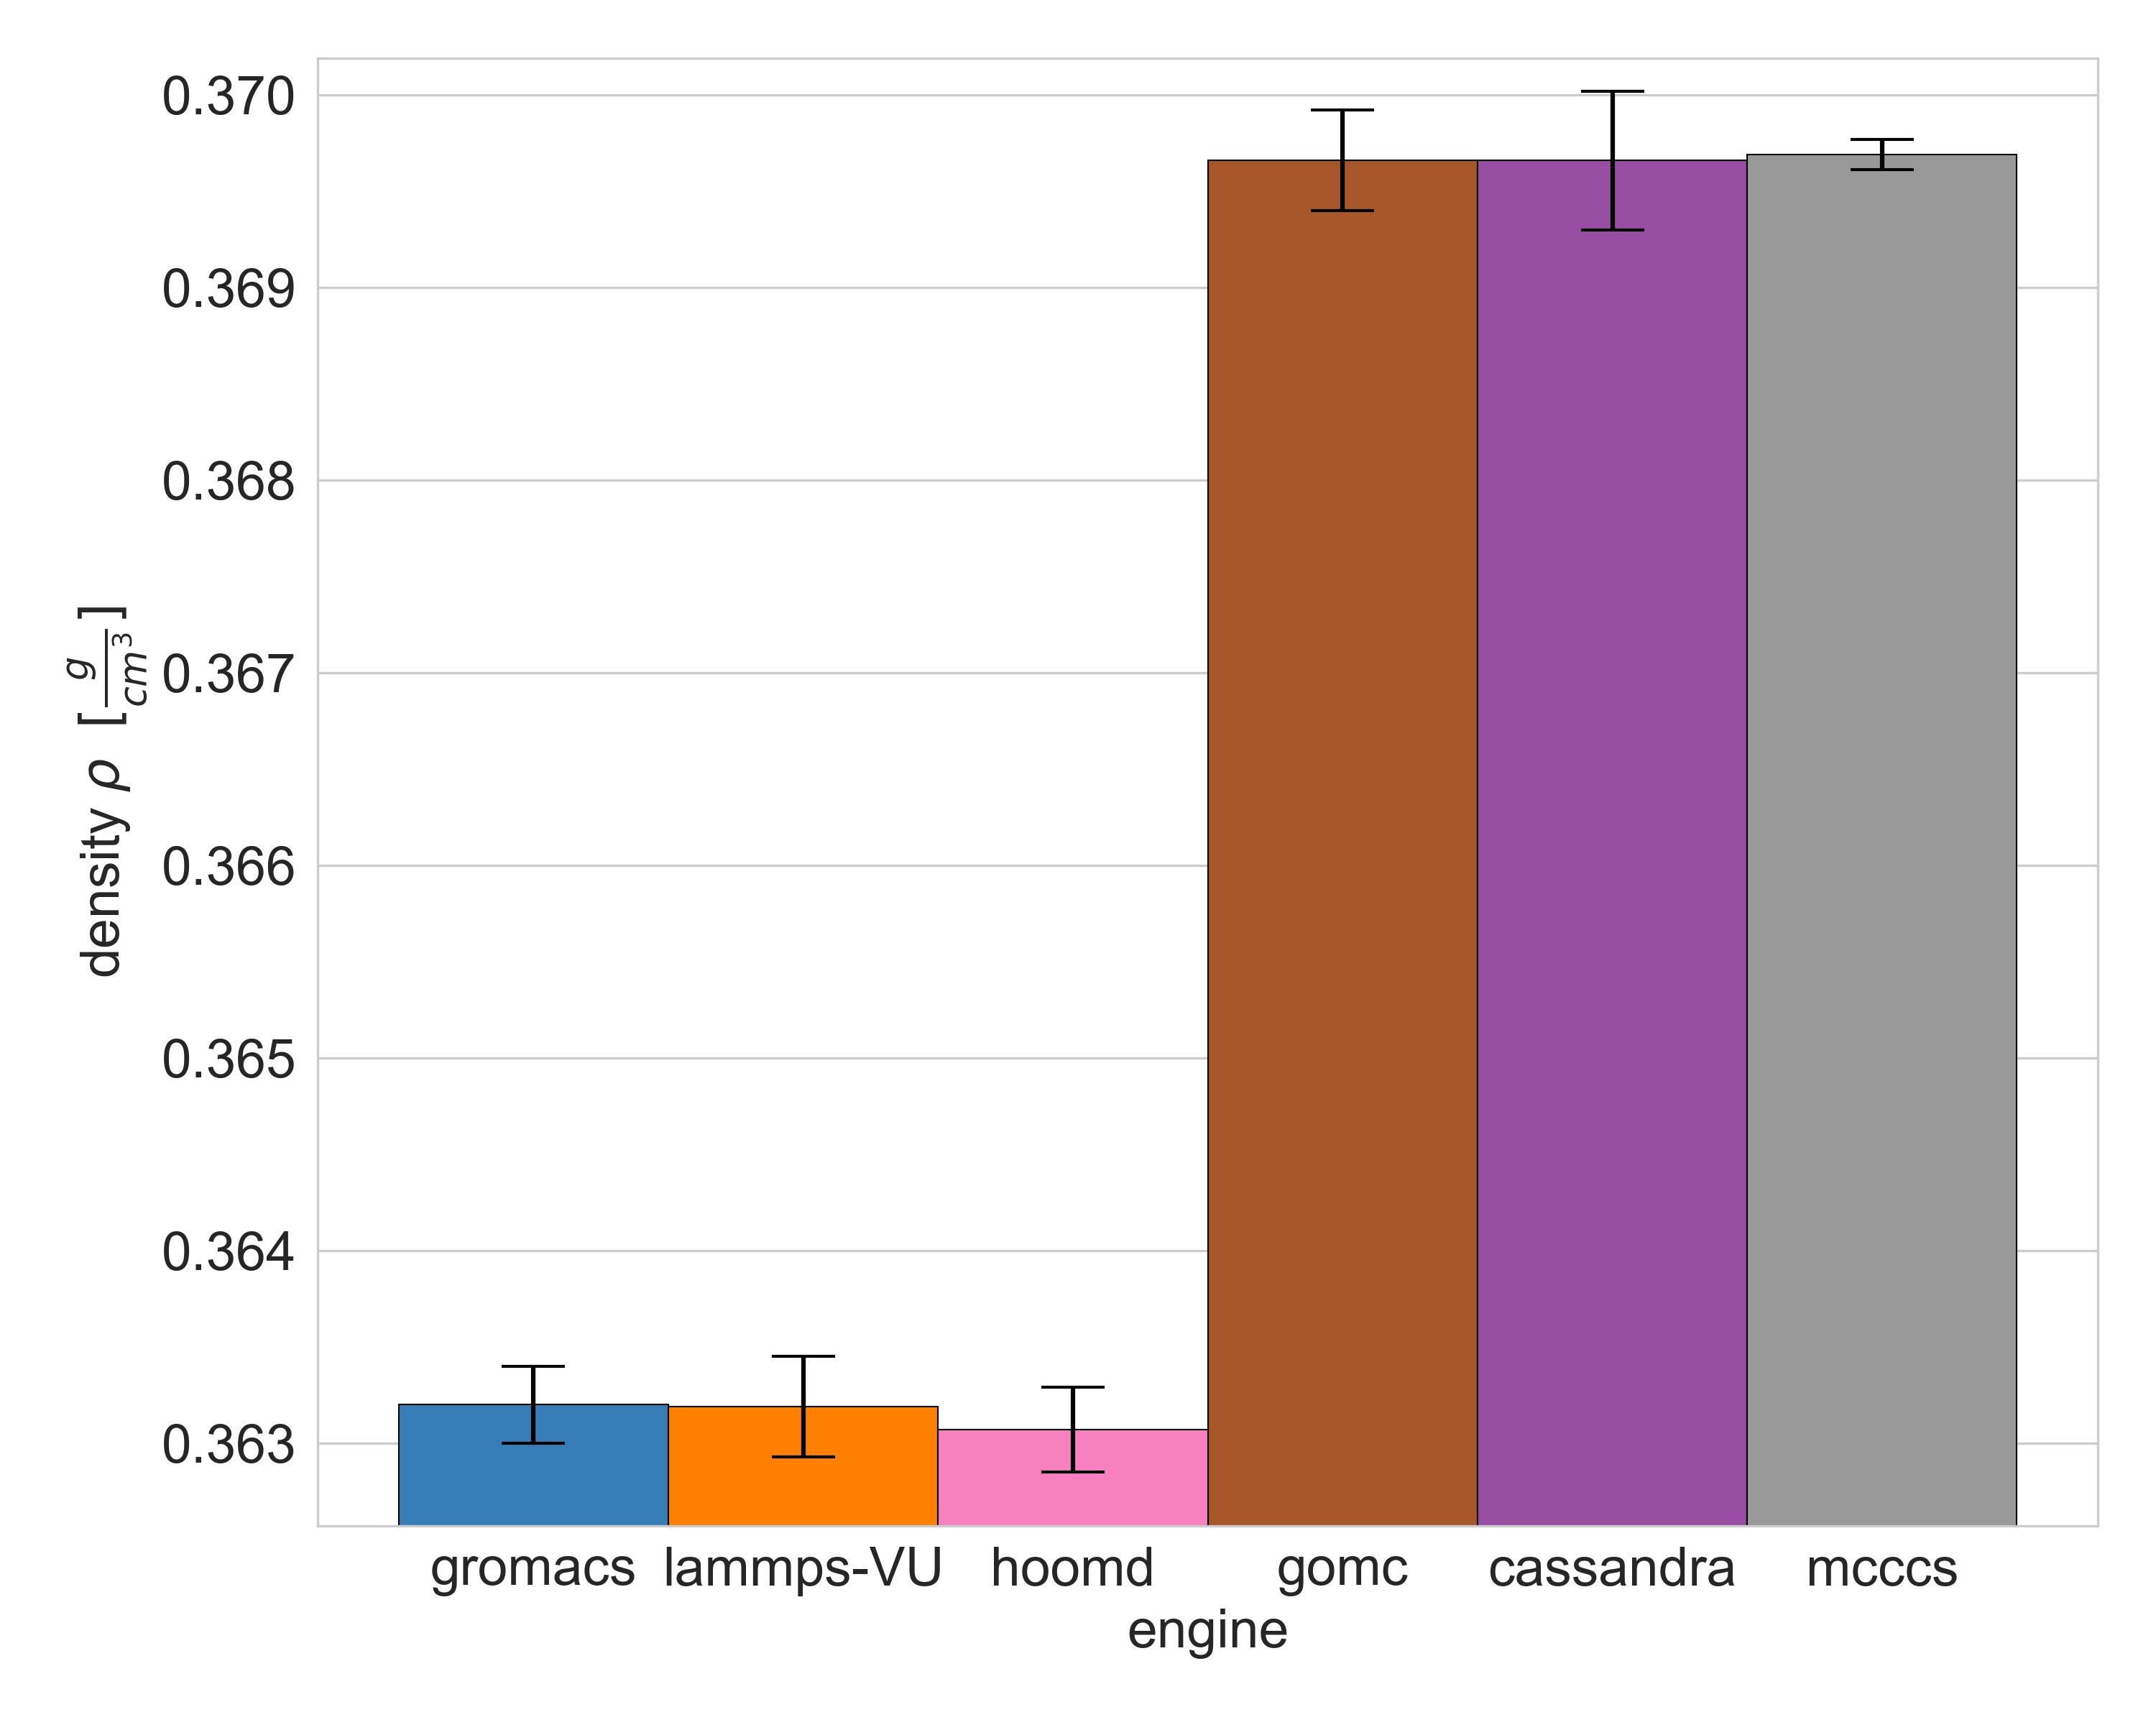
\includegraphics[width=0.6\linewidth,keepaspectratio]{figures/rep_study/hard_cutoff.png}
    \caption{Average density from NPT simulation of methane using "hard" cutoff by engine. The average is taken from independent samples of the equilibrated regions of 16 replicates. The error bars represent two standard deviations in each direction.}\label{fig:hard_cutoff}
\end{figure}
% Some MC engines use an impulsive contribution to the pressure which is not accounted for in MD and this may have some effect \citep{frenkel2001understanding}.
The variation in densities between MC and MD when using the hard cutoff scheme is most likely due to innate differences in the two methods: MD calculates the interparticle forces---the derivative of the potential with respect to r---and uses these forces to update the particle velocities and, in turn, positions. MC, however, calculates the potential values outright and uses the change in potential to choose whether to accept or reject a particular move.
Using a hard cutoff would cause a discontinuity in the potential, which results in how the force is handled near the cutoff to be ill-defined.

When a shifted cutoff is used (see \autoref{fig:shift_cutoff}), all engines equilibrate to the same density within error, but the density is much lower than the predicted value---the density of methane at 140K and 1318kPa is predicted to be 0.37808 g/cm$^3$\cite{NISTwebbook}.
\begin{figure}[h!]
    \centering
    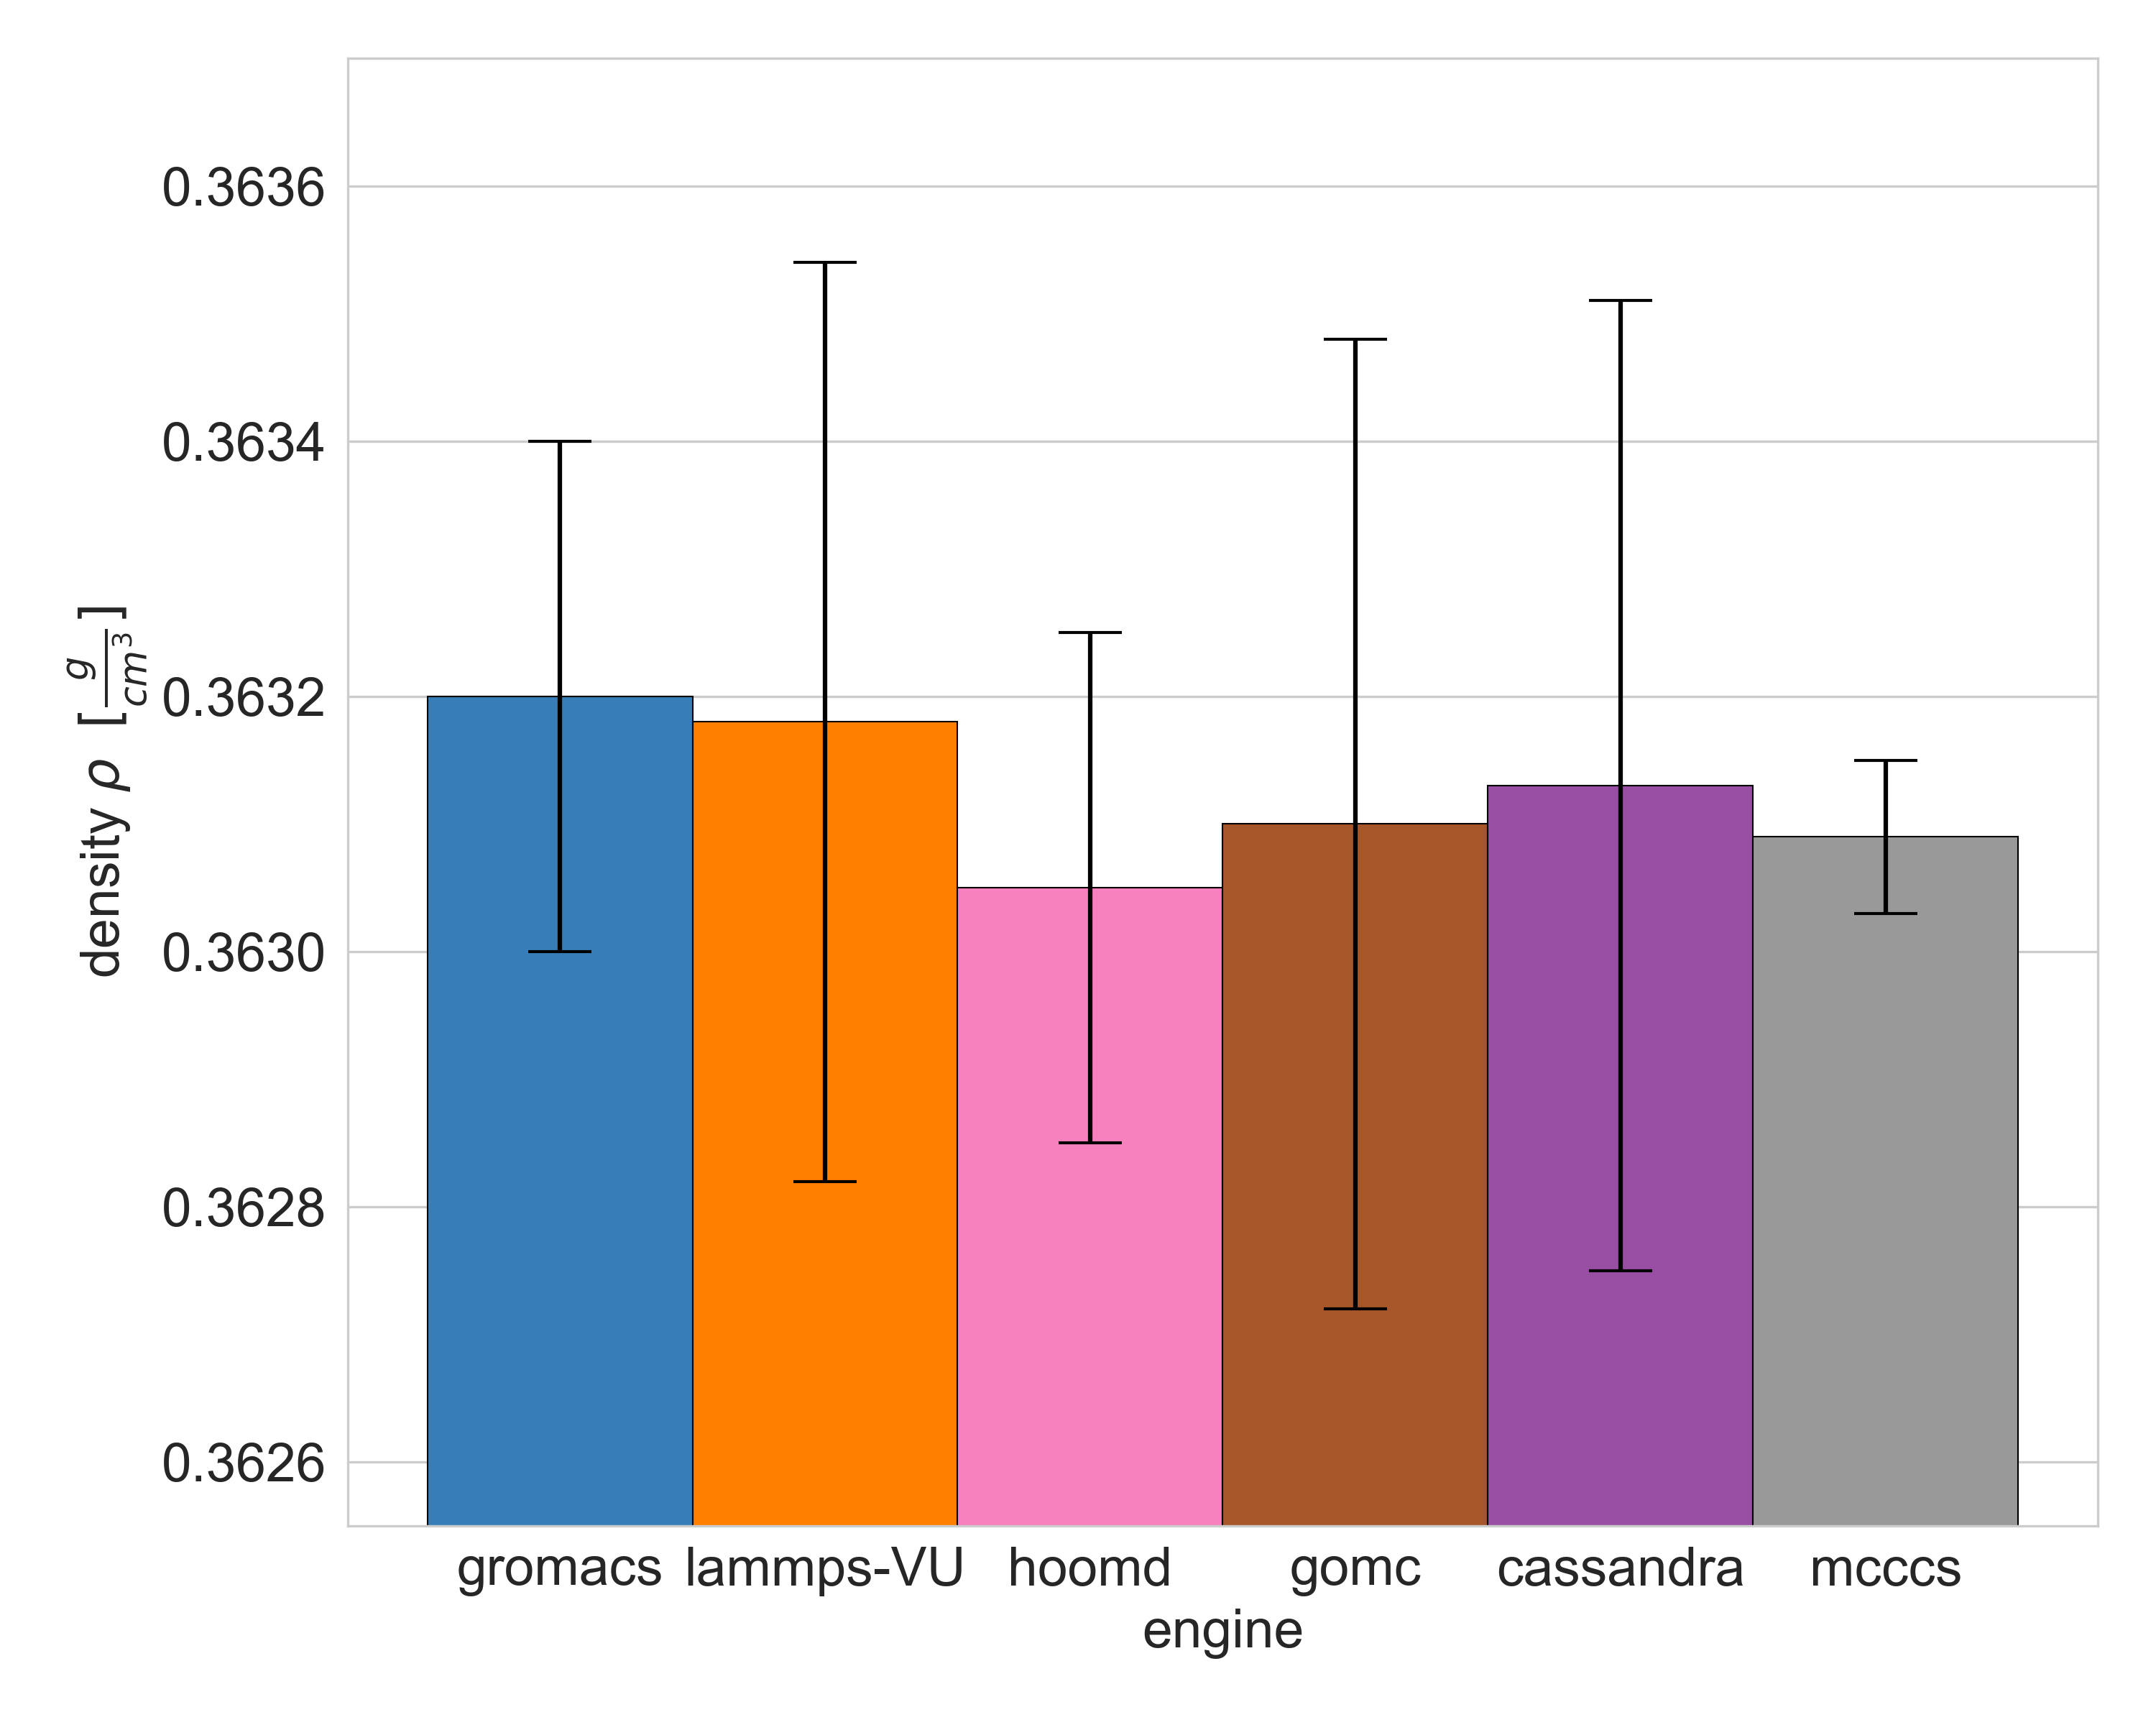
\includegraphics[width=0.6\linewidth,keepaspectratio]{figures/rep_study/shift_cutoff.png}
    \caption{Average density from NPT simulation of methane using "shifted" cutoff by engine. The average is taken from independent samples of the equilibrated regions of 16 replicates. The error bars represent two standard deviations in each direction.}\label{fig:shift_cutoff}
\end{figure}
This deviation from the correct density is due to the absolute values of the potential being shifted. 
Therefore the potential is different than it was originally created and parameterized, so it may yield different results.
(The TraPPE-UA forcefield, for example, was designed to be used with analytical tail corrections as described in Equations~\eqref{lrc_e} and \eqref{lrc_p}.)

In order to get consensus between engines and closer to the correct density value, the correction to the energy and pressure was needed (see \autoref{fig:lrc_cutoff}).
\begin{figure}[h!]
    \centering
    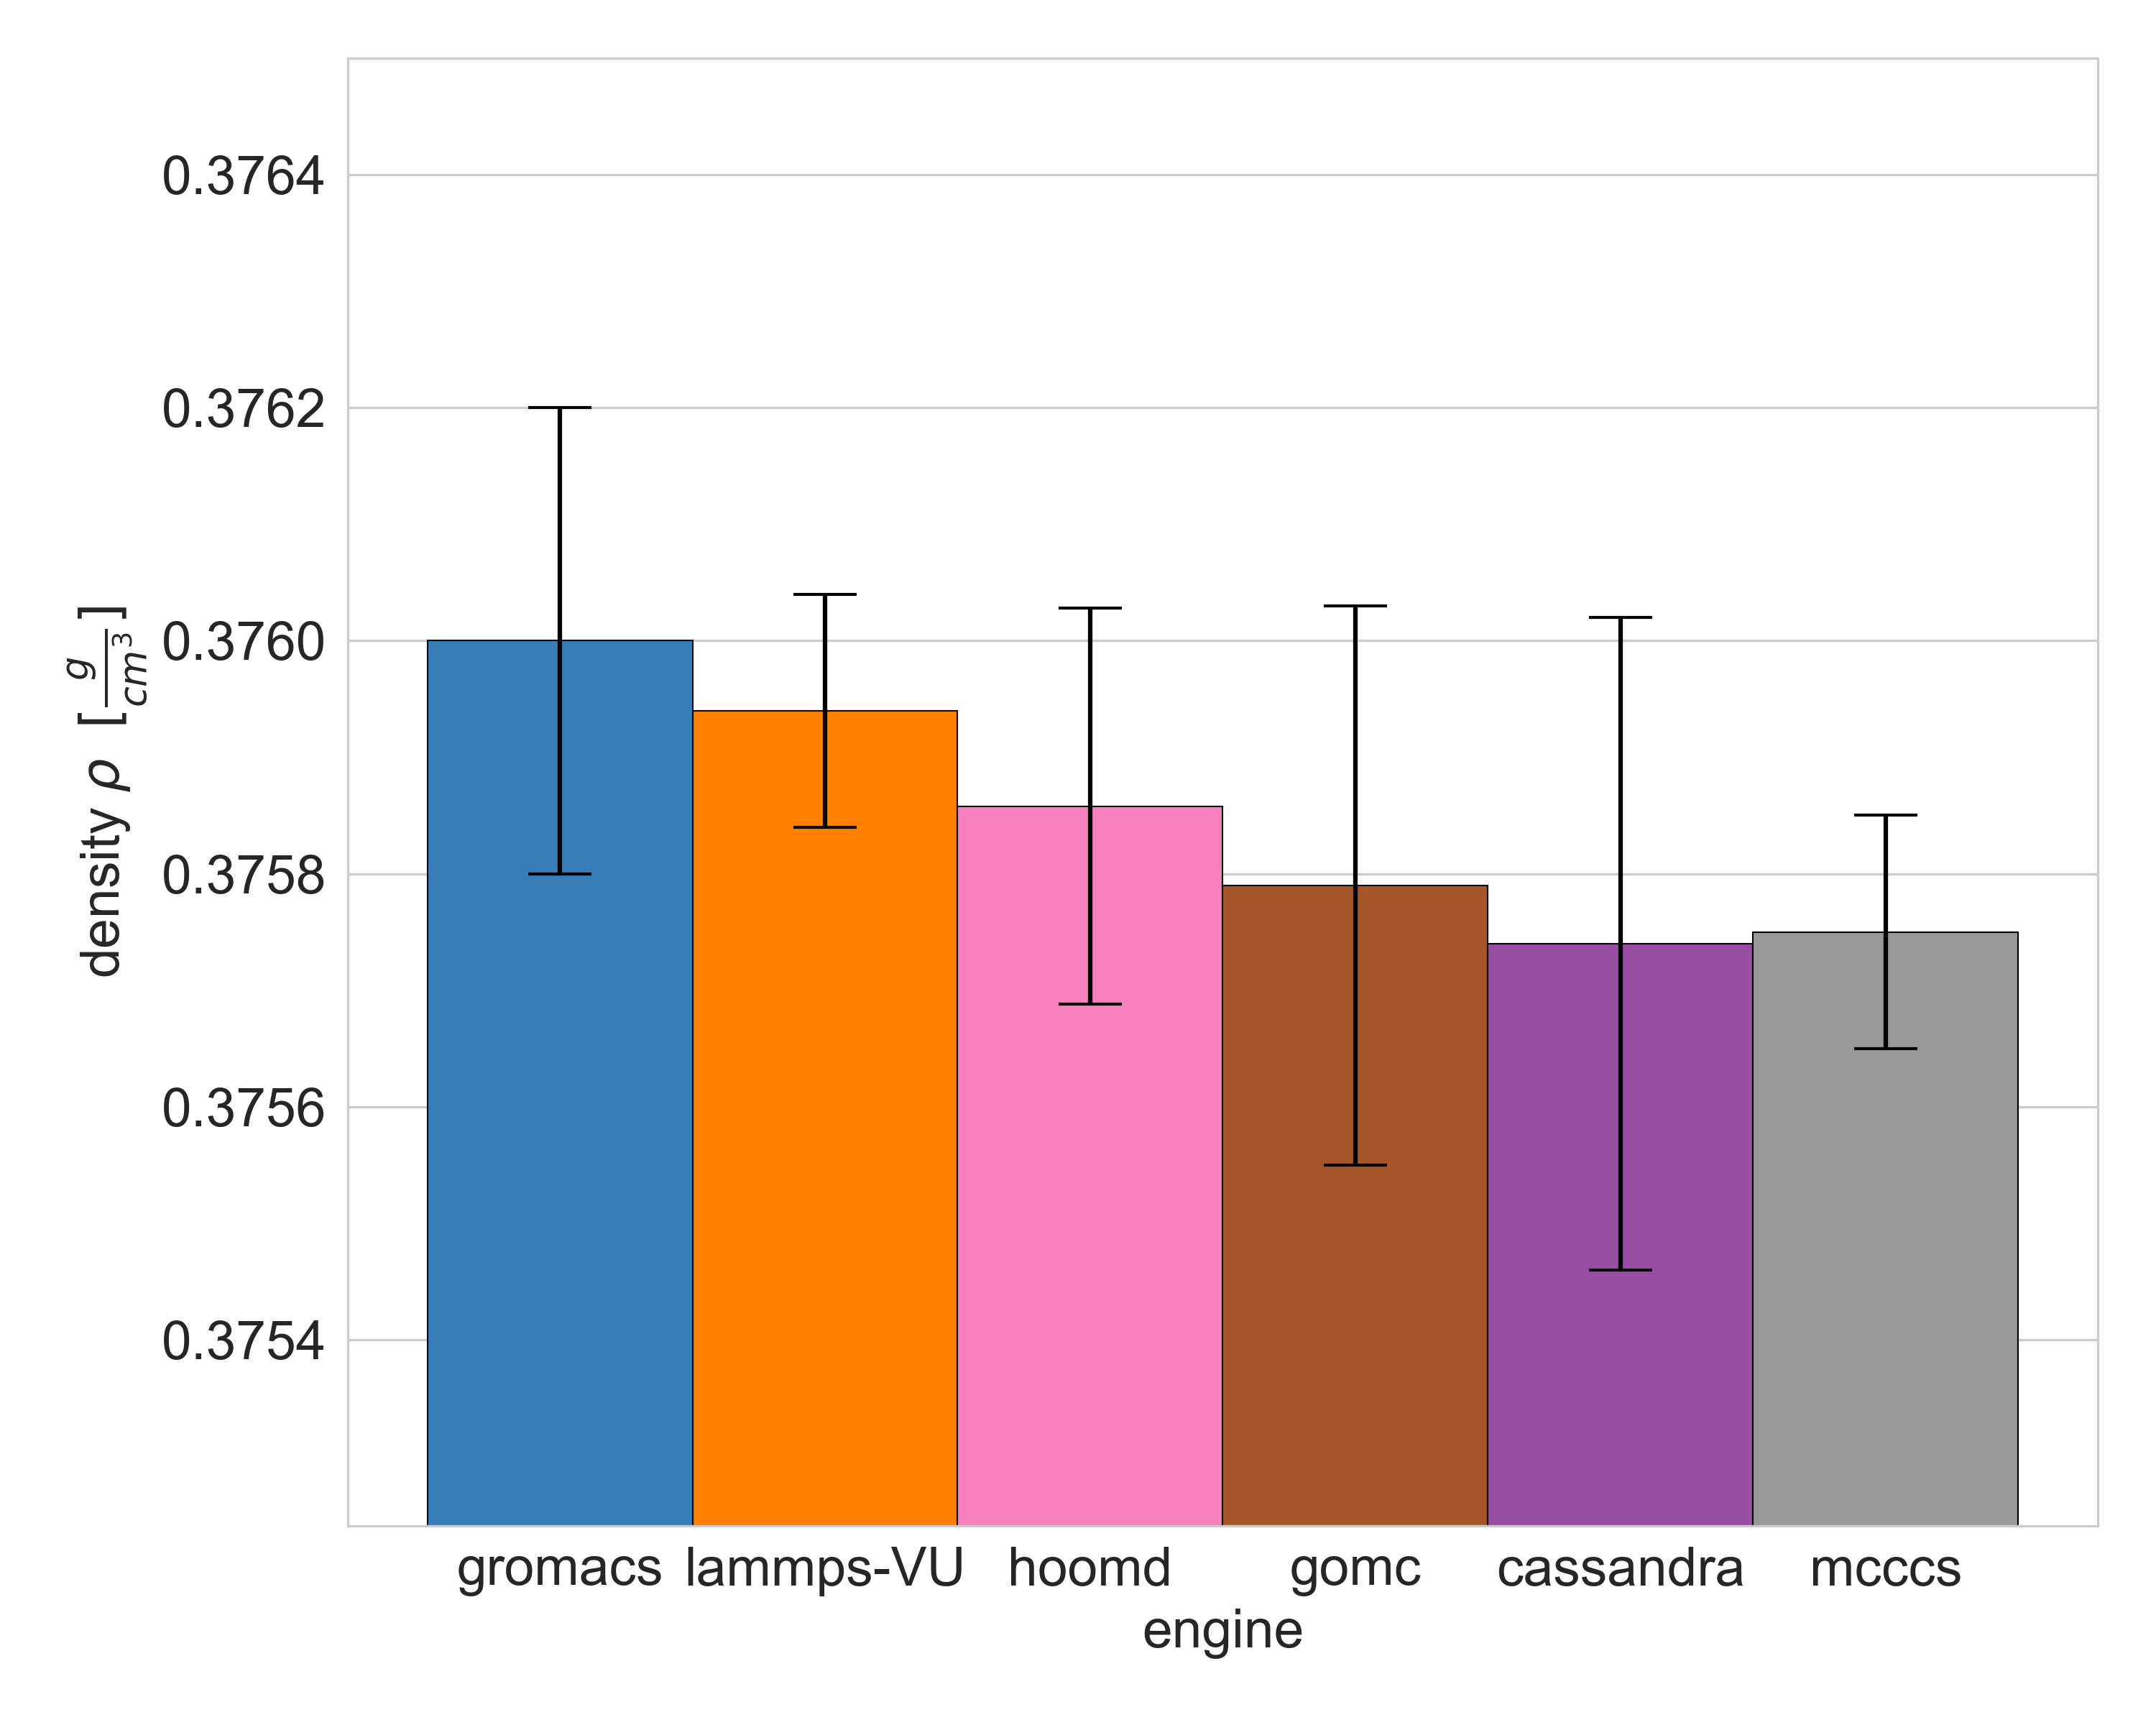
\includegraphics[width=0.6\linewidth,keepaspectratio]{figures/rep_study/lrc_cutoff.png}
    \caption{Average density from NPT simulation of methane using energy and pressure long range correction by engine. The average is taken from independent samples of the equilibrated regions of 16 replicates. The error bars represent two standard deviations in each direction.}\label{fig:lrc_cutoff}
\end{figure}
By using the energy-pressure correction, the energies and densities of both MD and MC are within the error tolerance of two standard deviations. 

It is worth noting that differences in the computed pressure exist between engines regardless of cutoff scheme, see \autoref{fig:lrc_pressure}.
\begin{figure}[h!]
    \centering
    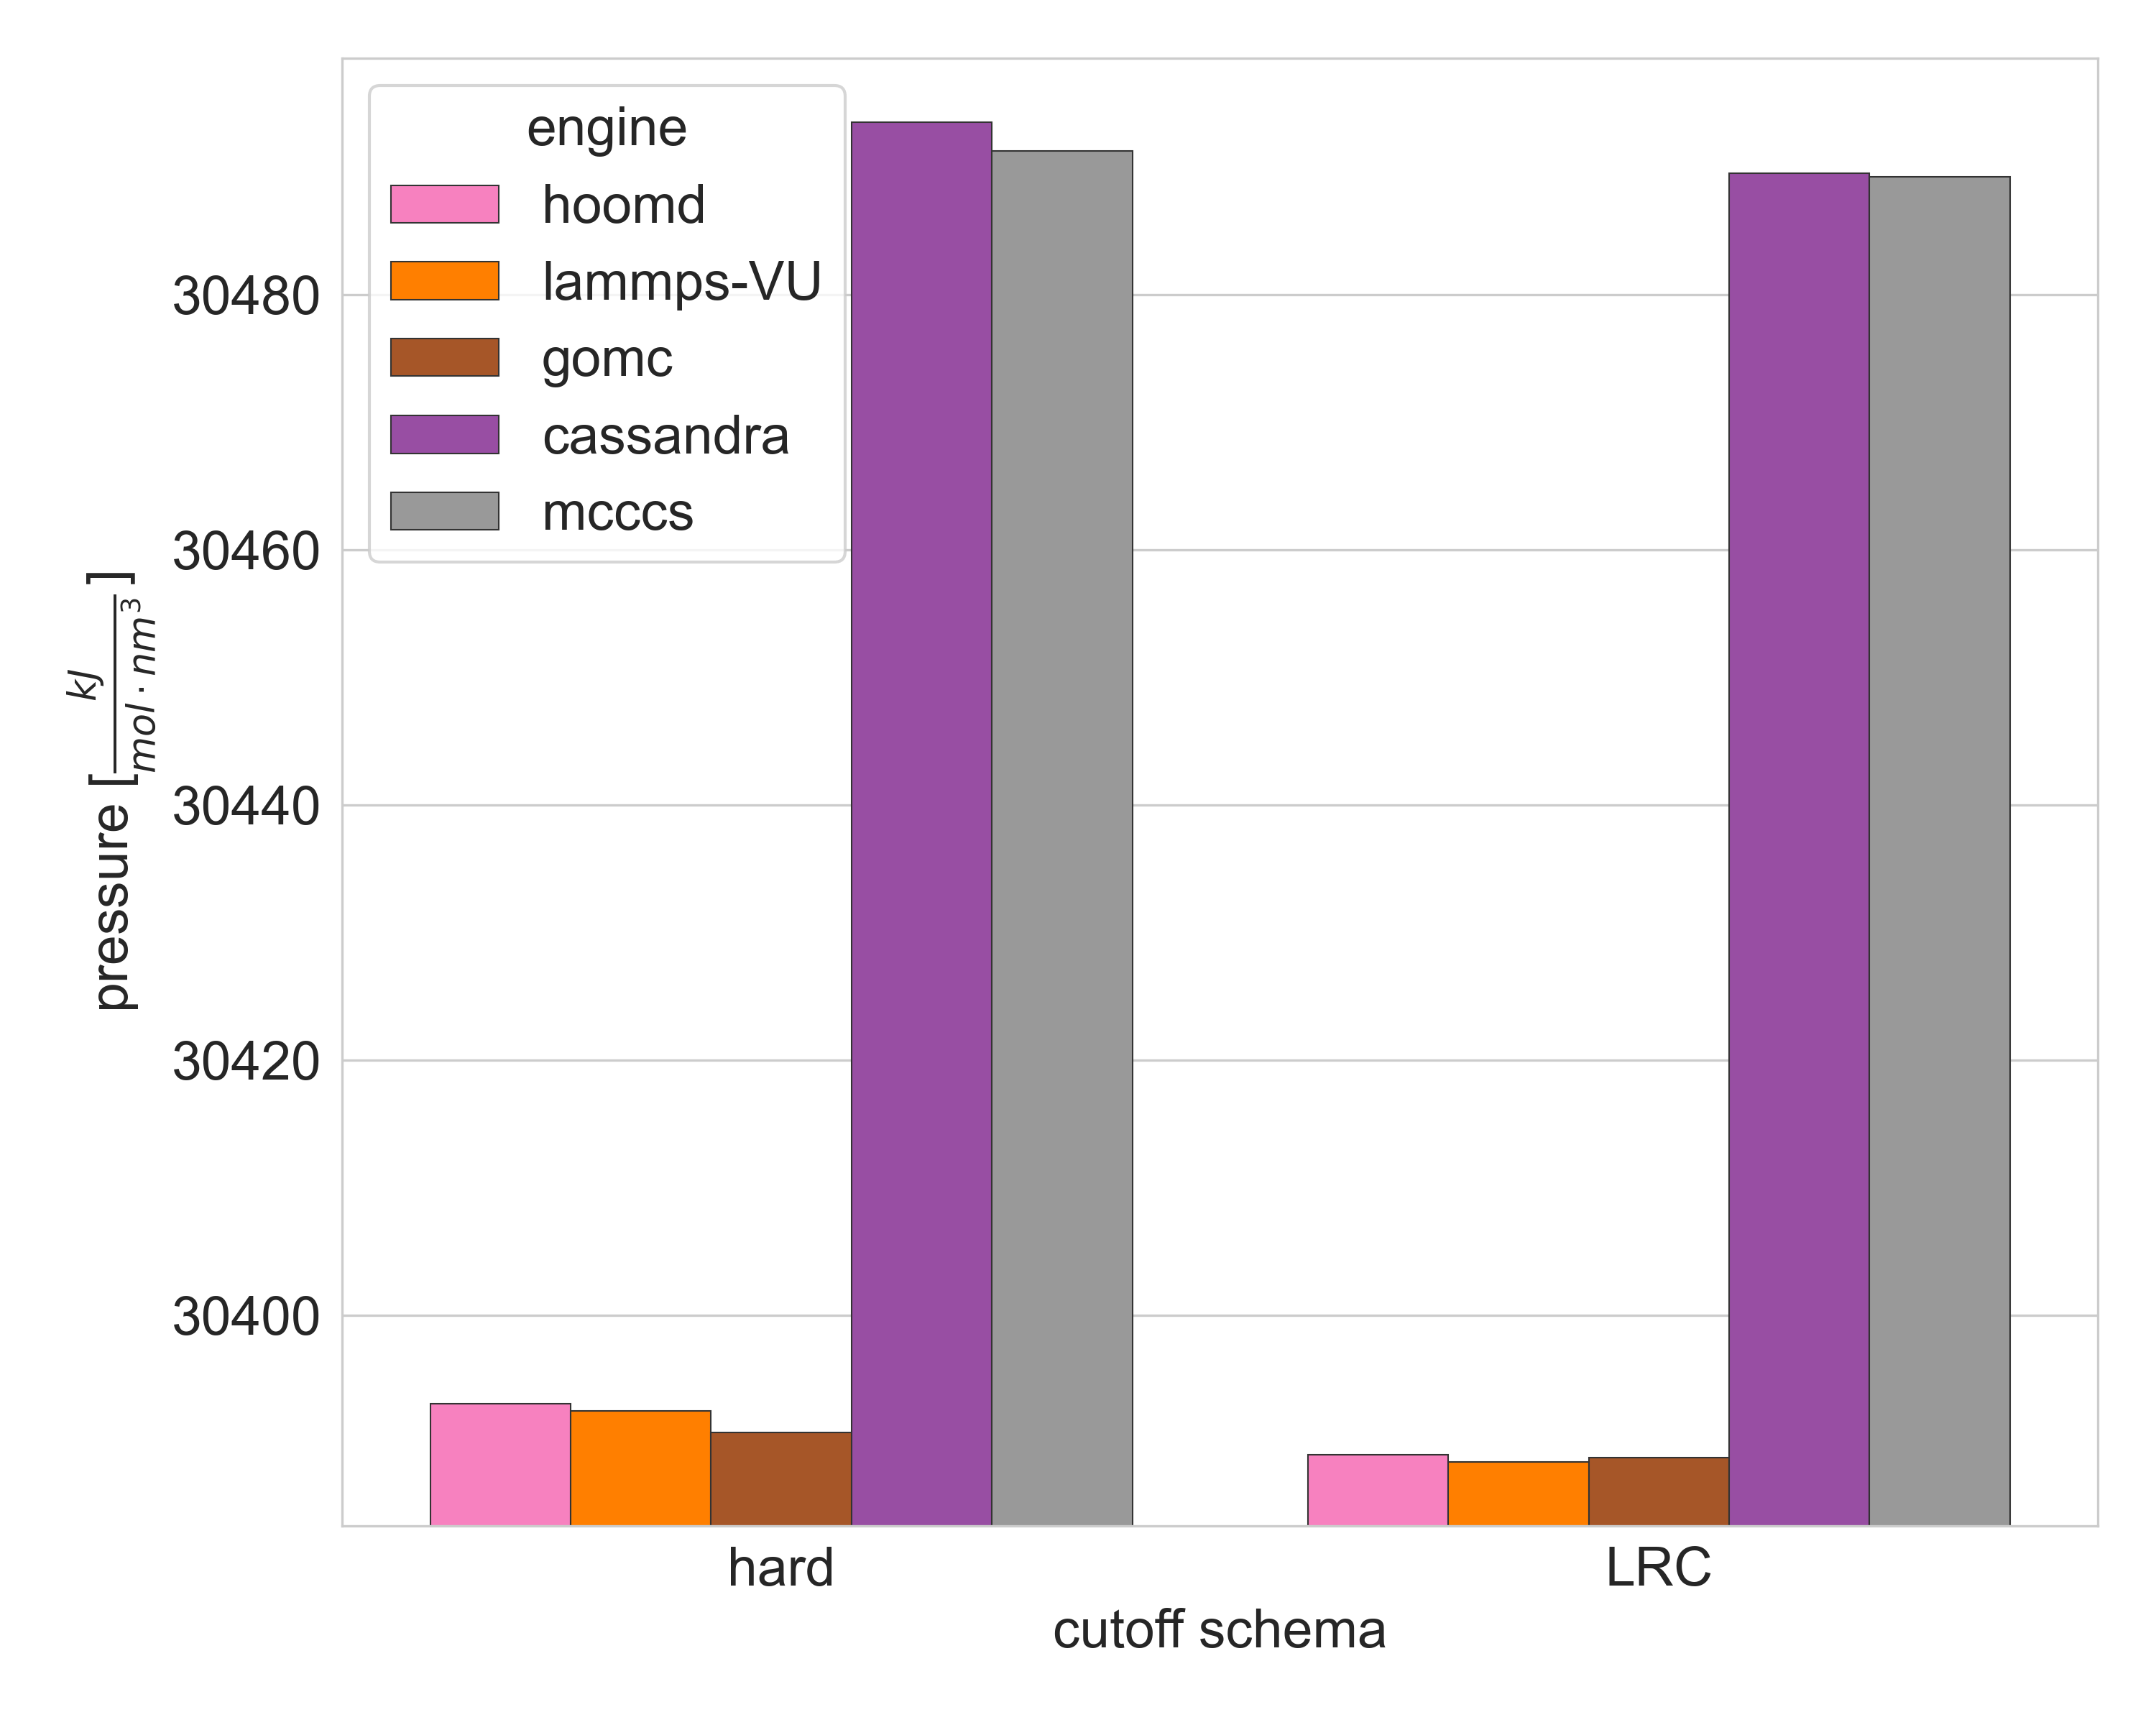
\includegraphics[width=0.6\linewidth,keepaspectratio]{figures/rep_study/lrc_pressure.png}
    \caption{Instantaneous pressure from first frame of methane by engine comparing "hard" and "LRC" cutoff schemes.}\label{fig:lrc_pressure}
\end{figure}
These discrepancies in pressure may be due to the ideal gas contribution to pressure. 
The pressure in molecular simulation can be computed by the following equation
\begin{equation}\label{eq:pressure}
    P = \frac{N k_{B} T}{V} + \frac{\sum_{i}^{N^{'}} r_{i} \cdot f_{i}}{dV}
\end{equation}
where $N$ is the number of atoms, $k_{B}$ is Boltzmann's constant, $T$ is the temperature, $d$ is the dimensionality of the system, $V$ is the system volume, and $r_i$ and $f_i$ are the position and force vectors of atom $i$ \citep{Thompson2009}.
The first term in \autoref{eq:pressure} is the ideal gas contribution to pressure.
Not including this ideal gas contribution is akin to calculating the pressure of the system at 0K.
HOOMD calculates the pressure with the virial equation which includes accounting for the translational kinetic energy, essentially the kinetic temperature.
However, calculating the pressure difference due to the ideal gas contribution from 900 particles at 140 K in a 63.9 nm$^3$ box accounts for a difference of about 16 $\frac{kJ}{mol \cdot nm^{3}}$ while \autoref{fig:lrc_pressure} shows the discrepancy is closer to 100 $\frac{kJ}{mol \cdot nm^{3}}$, so further investigation into the source of this discrepancy is required.

Through examination of the energy values of this first frame we also found a discrepancy in the energies reported in newer versions of GROMACS, see \autoref{fig:lrc_energy}.
\begin{figure}[h!]
    \centering
    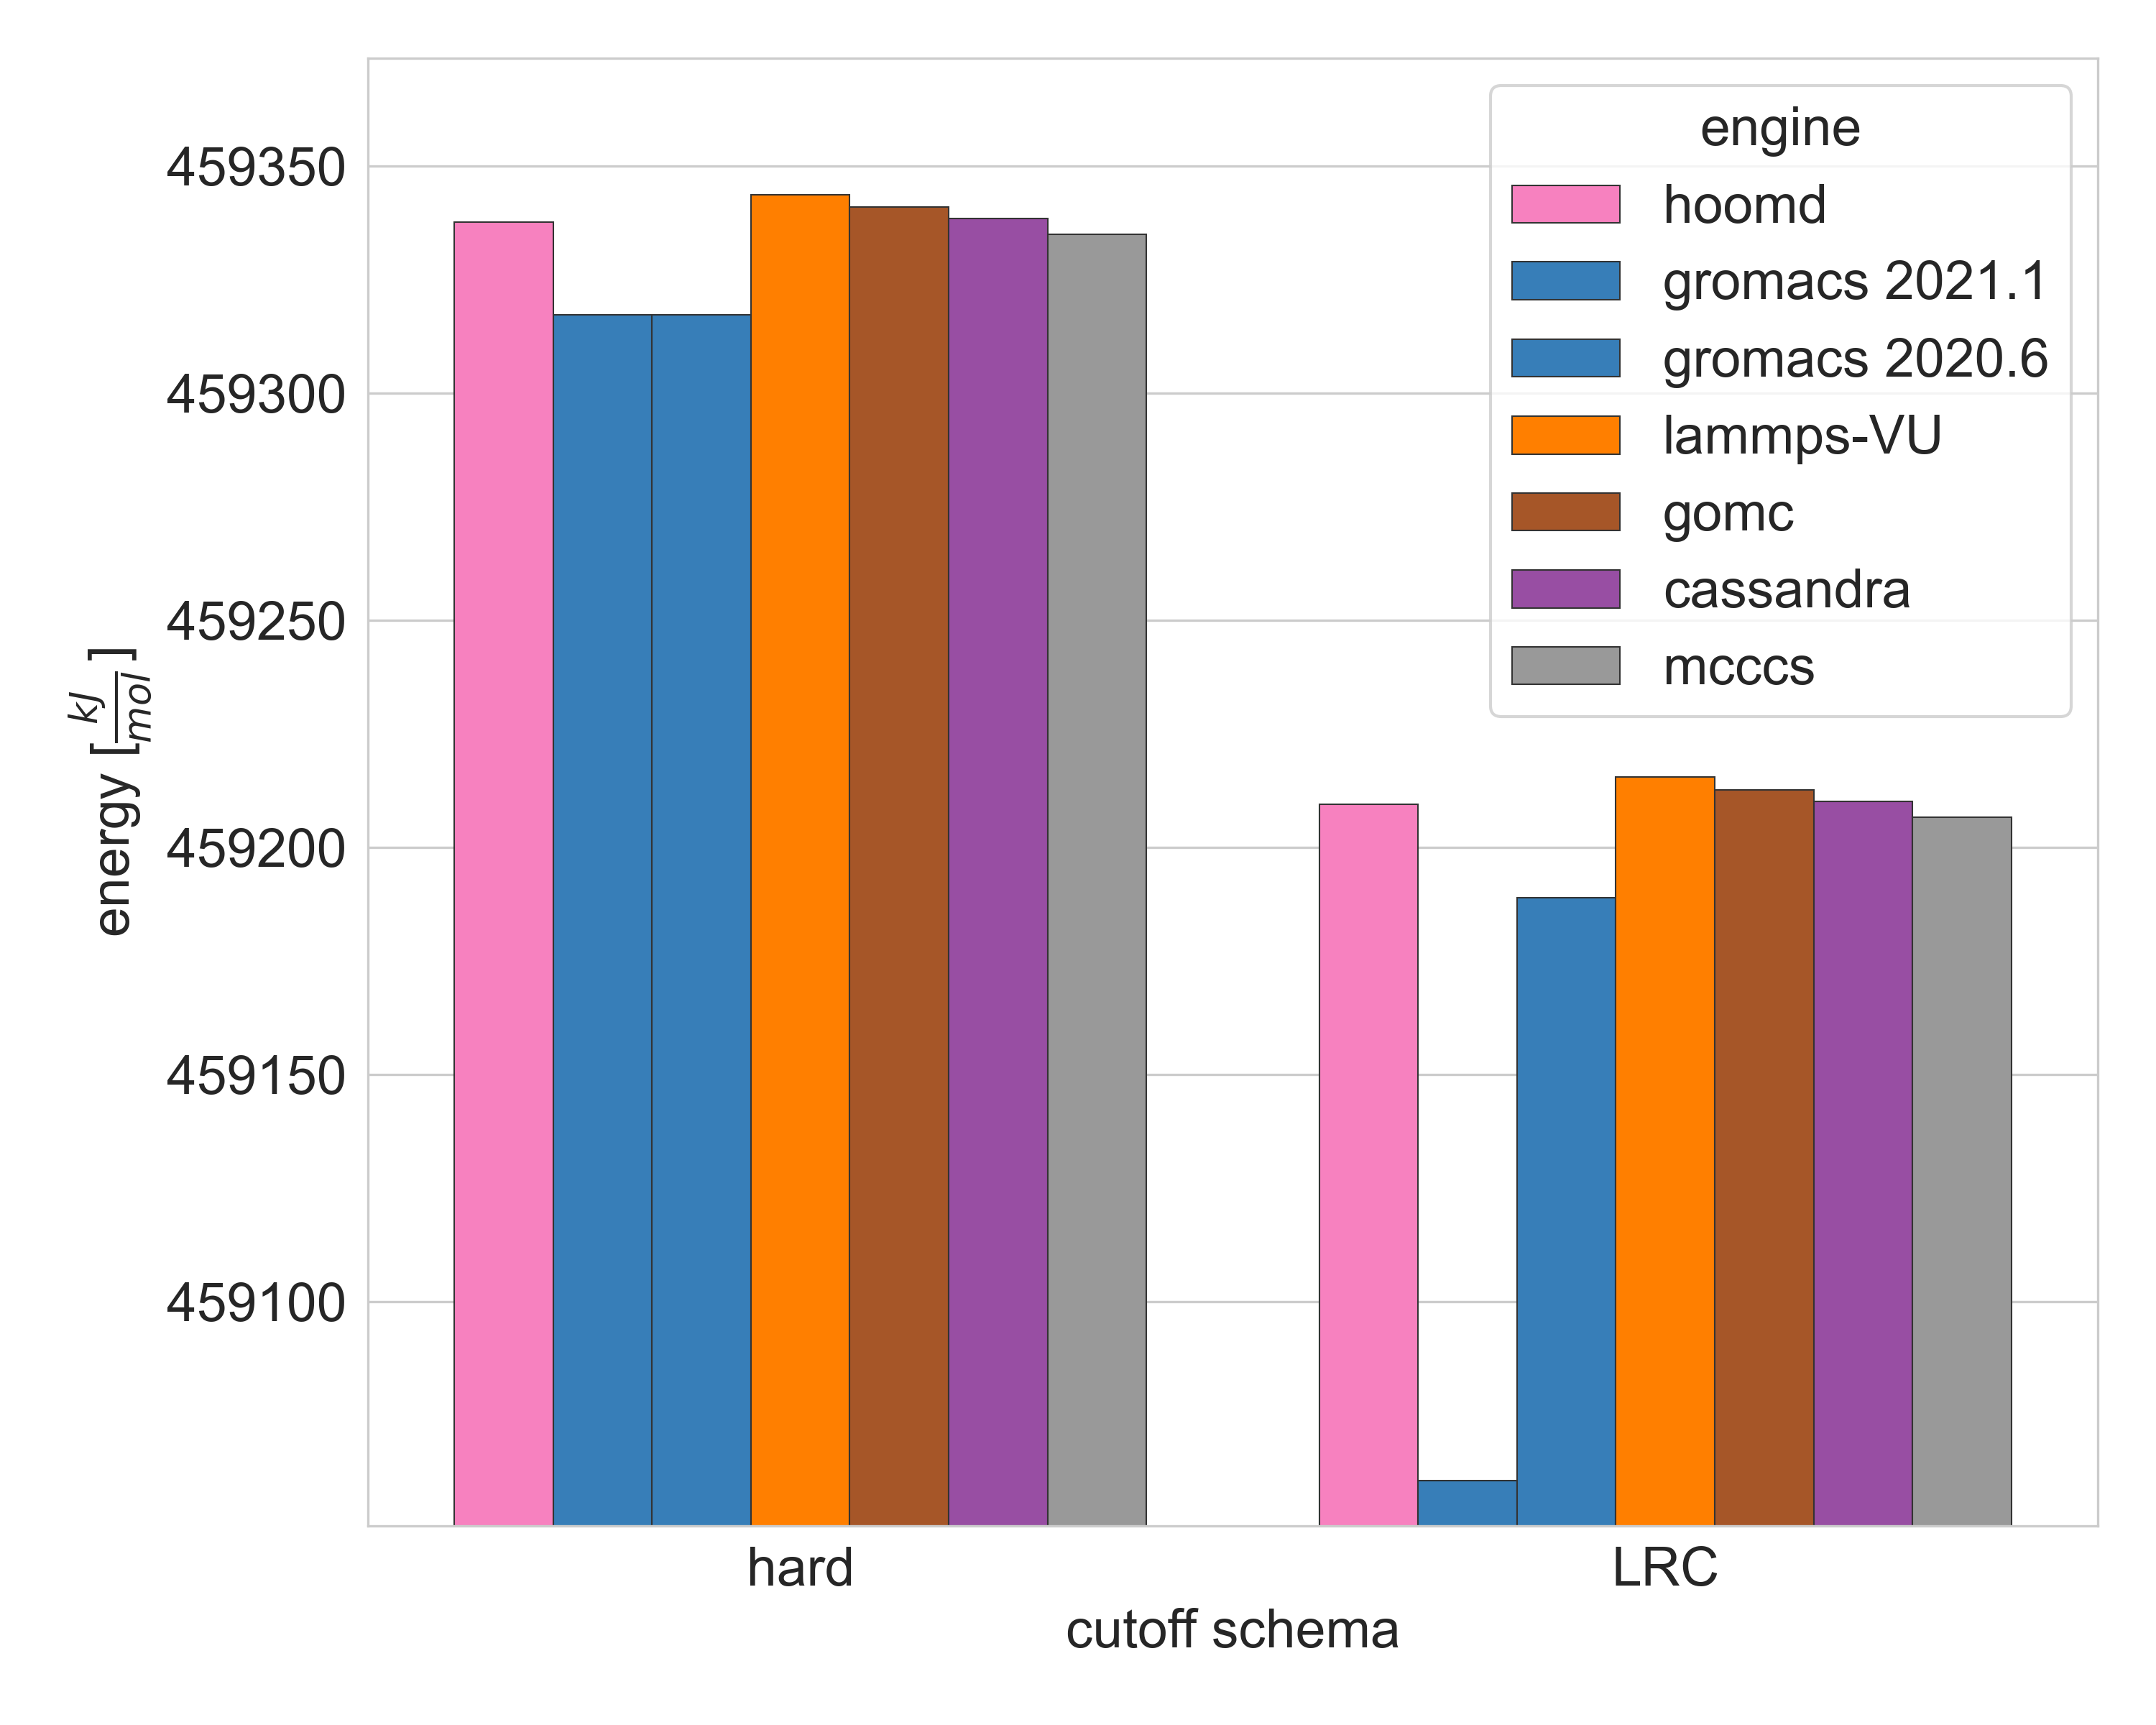
\includegraphics[width=0.6\linewidth,keepaspectratio]{figures/rep_study/lrc_energy.png}
    \caption{Instantaneous energies from first frame of methane by engine comparing "hard" and "LRC" cutoff schemes.}\label{fig:lrc_energy}
\end{figure}
This should not have an effect on the end result but is worth noting for those who may want to compare instantaneous energies:
Newer versions of GROMACS do not include the pressure correction to energy in the total potential energy when running an energy minimization step. 
This is documented in \href{https://gitlab.com/gromacs/gromacs/-/issues/4229}{GROMACS Issue 4229}.

Although it may seem of little significance, the choice of where the cutoff is set and how the cutoff is handled can greatly affect the simulation outcome.

\subsection{Rigid constraints}

Benzene and water are modelled as rigid bodies in this study.
In HOOMD, rigid bodies consist of a central body particle and its constituent particles. 
All of these particles can have forces acting upon them, but the mass and moment of inertia of the body particle is set to be the full mass and moment of inertia of the body plus its constituents.  
Further description of how the rigid constraint forces are implemented can be found in \citet{Nguyen2011a} and \citet{Glaser2020a}, and I contributed to updating the rigid body constraint to the v3 api.
HOOMD provides functions to simplify the initialization of rigid bodies; however, using these rigid body functions with MoSDeF tools introduced additional hurdles. 
The difficulties which arise at the intersection between codebases are those with which many simulators will be familiar.

Initializing rigid bodies in HOOMD using MoSDeF tools required additional effort, as there are some idiosyncrasies that conflict with the typical workflow.
In order to initialize a rigid body in HOOMD, all the body particles must be first in the snapshot and the constituent particles must all have the same relative orientation to the body particle. 
To reduce the cognitive load for users, HOOMD recommends creating the body constituent particles using the \lstinline{create_bodies} function, but this precludes using the MoSDeF initialization functions which fill the simulation volume, apply the forcefield, and initialize the HOOMD forces.
Therefore, we have developed a generalized workflow based on the assumption that each molecule is the same and will be its own rigid body.
First, an initial snapshot is created with the same number of body particle as molecules.
Using a functionality which I contributed to the \lstinline{create_hoomd_forcefield}, this initial snapshot can be passed in and the normal workflow---filling the box with all molecules in the same orientation and applying the forces---can add on to this initial snapshot. 
Next, the number of molecules and the number of particles in each molecule is used index through the snapshot to set the body ids for each constituent particle and to calculate and set the position, mass, and moment of inertia tensor for each body particle.
Finally, the body constraint is defined based on the types, charges, diameters, and relative positions and orientations, of the first molecule.

Before using rigid bodies for water and benzene, the HOOMD simulations were taking an excessive amount of time to equilibrate and were equilibrating to vastly different results as other engines.
There was some hesitation to use rigid bodies because it was a function that was not supported or implemented differently in other engines.
However \autoref{fig:benzene_density} and \autoref{fig:water_density} suggest that the rigid models achieve agreement.

Currently the example for initializing rigid bodies in the HOOMD v3 API is still under development.
This workflow can serve as an example of how run simulations of rigid bodies in HOOMD using MoSDeF tools.

\section{Results} 

This study is still underway and data is still being collected, however we will examine the current results of this study up to this point, namely the densities and potential energies.
First let's start with the simplest system, UA methane.
The density of methane between engines agrees within error (see \autoref{fig:methane_density}).
\begin{figure}[h!]
    \centering
    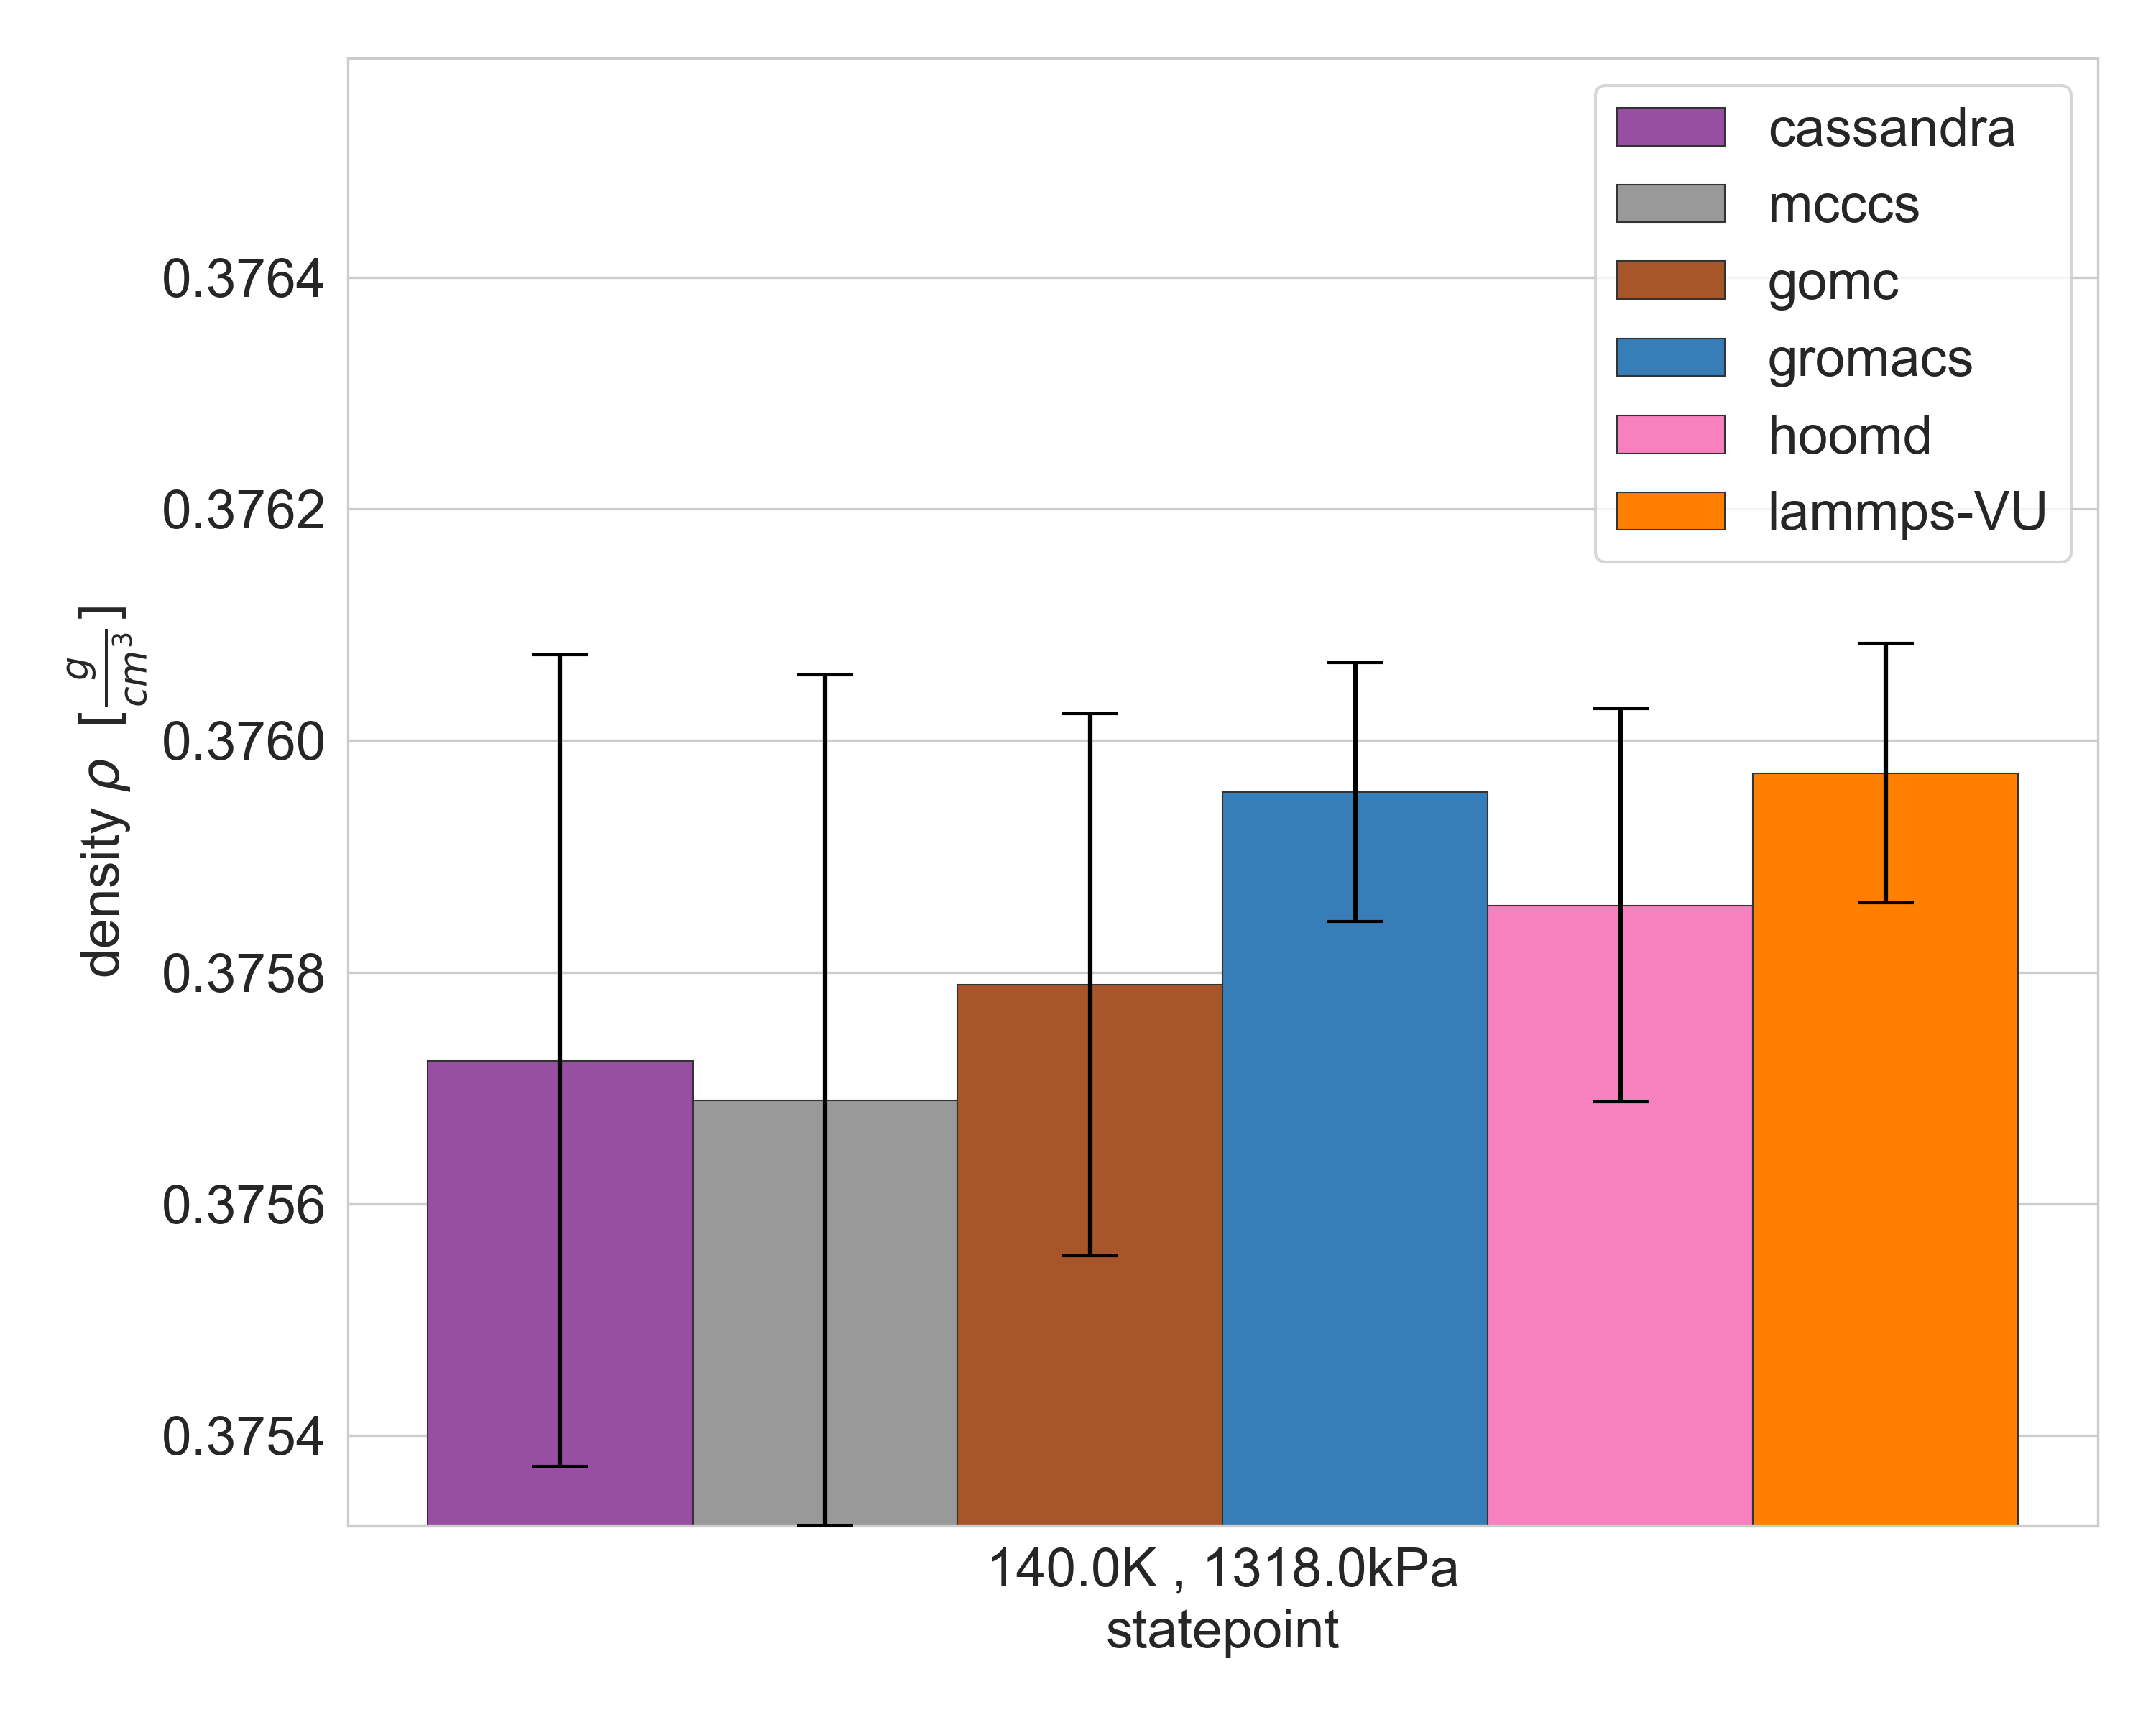
\includegraphics[width=0.6\linewidth,keepaspectratio]{figures/rep_study/methaneUA_summary.png}
    \caption{Average density of methane by engine. The average is taken from independent samples of the equilibrated regions of 16 replicates. The error bars represent two standard deviations in each direction.}\label{fig:methane_density}
\end{figure}
The MC density and potential energy data shows higher variation than the MD results. %due to the randomness of the MC moves resulting in more varied configurations, while the configurations in MD are more connected by their dynamics. 
It appears that the MC engines in general equilibrate to a lower density, perhaps because they can more easily sample high density configurations using unphysical moves (e.g., moving through objects, etc).
In contrast, MD may be more restricted by dynamics and must follow a physical path to reach a configuration, which could make getting to these high density configurations more difficult.
The predicted density of methane at 140 K and 1318 kPa should be around 0.37808 g/cm$^3$ \cite{NISTwebbook}.
We can see that the MD engines, which get closer to the predicted density, have a lower potential energy \autoref{fig:methane_pe}.
\begin{figure}[h!]
    \centering
    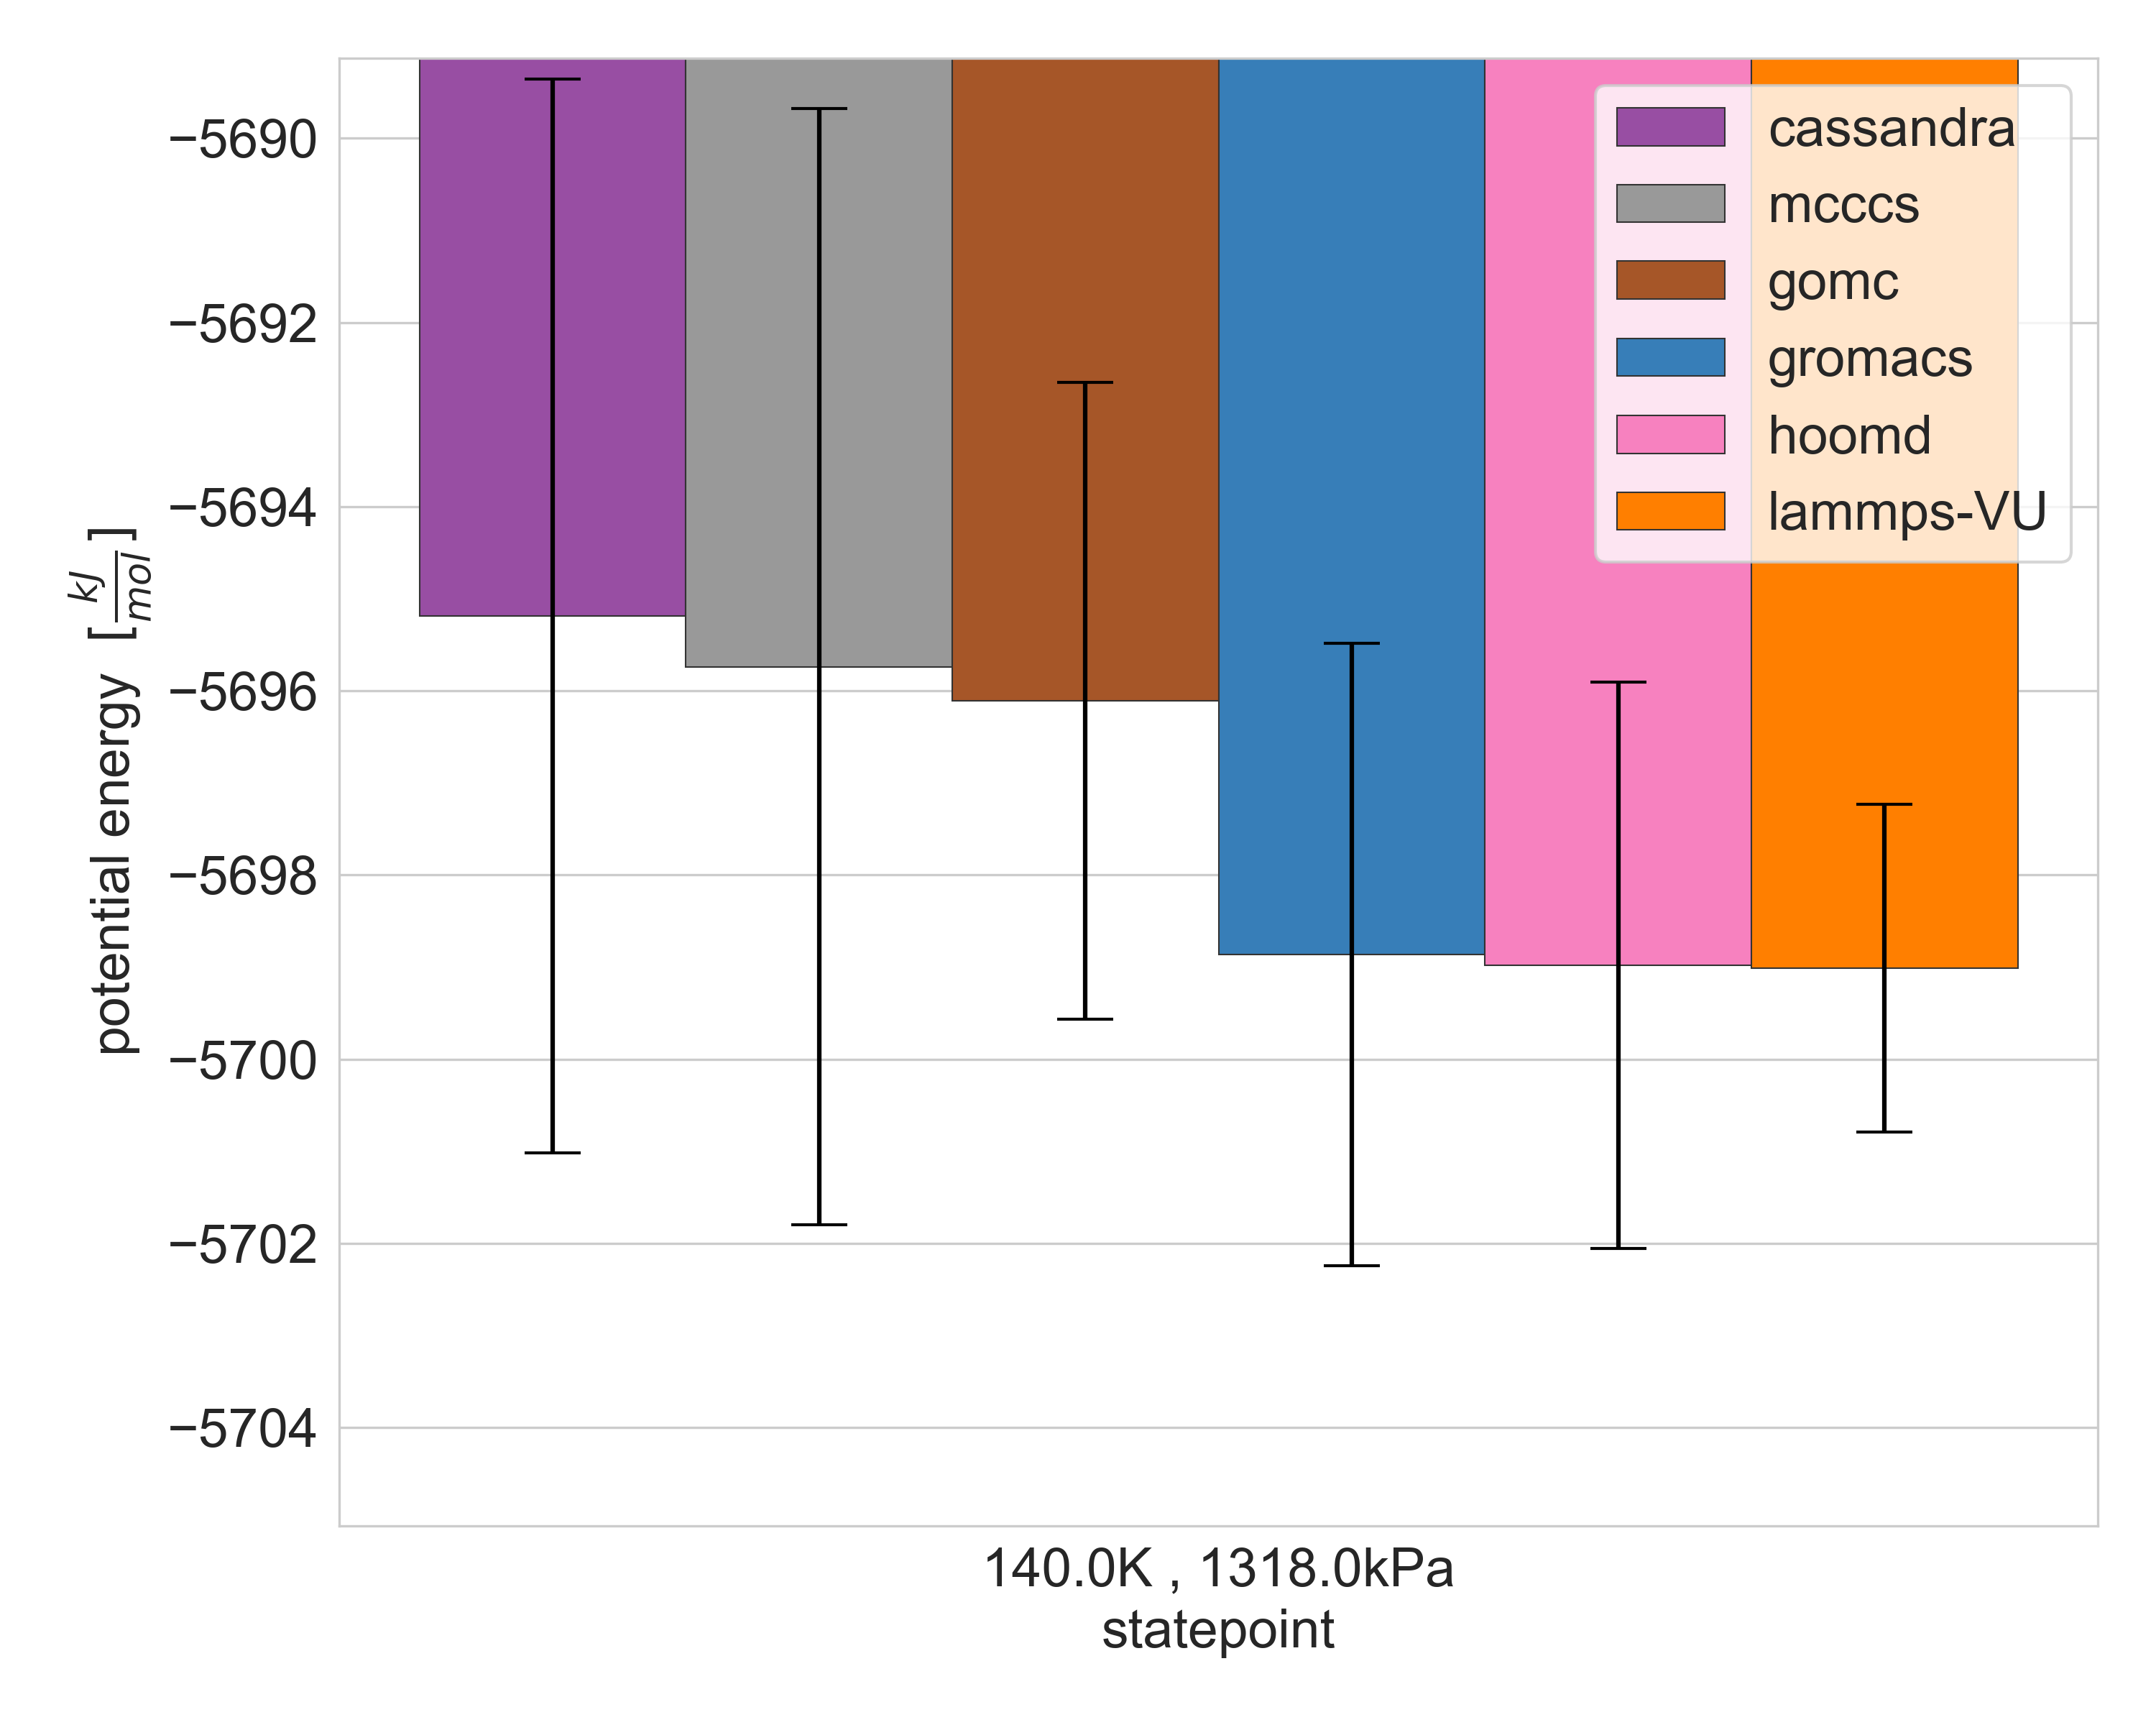
\includegraphics[width=0.6\linewidth,keepaspectratio]{figures/rep_study/methaneUA_pe_summary.png}
    \caption{Average potential energy of methane by engine. The average is taken from independent samples of the equilibrated regions of 16 replicates. The error bars represent two standard deviations in each direction.}\label{fig:methane_pe}
\end{figure}
%This makes sense: the distances between methane particles are likely on average closer to the equilibrium distance, which would result in a density closer to the predicted and a lower potential energy.
Although there are some differences we can see here between MD and MC, the potential energies of methane also agree between engines within error.

Next, let's examine UA pentane, which adds bond, angle, and dihedral forces. 
Within the pentane model, two bond types were used: flexible and fixed-length (also called constrained) bonds.
This choice was made because the MC engines only have the capability to model constrained bonds. 
Therefore, by modelling a single system in each way (for the engines which are able) we can isolate and observe the effect of bond type.
\autoref{fig:pentane_density} shows the densities of pentane with flexible and fixed bonds by engine.
\begin{figure}[h!]
    \centering
    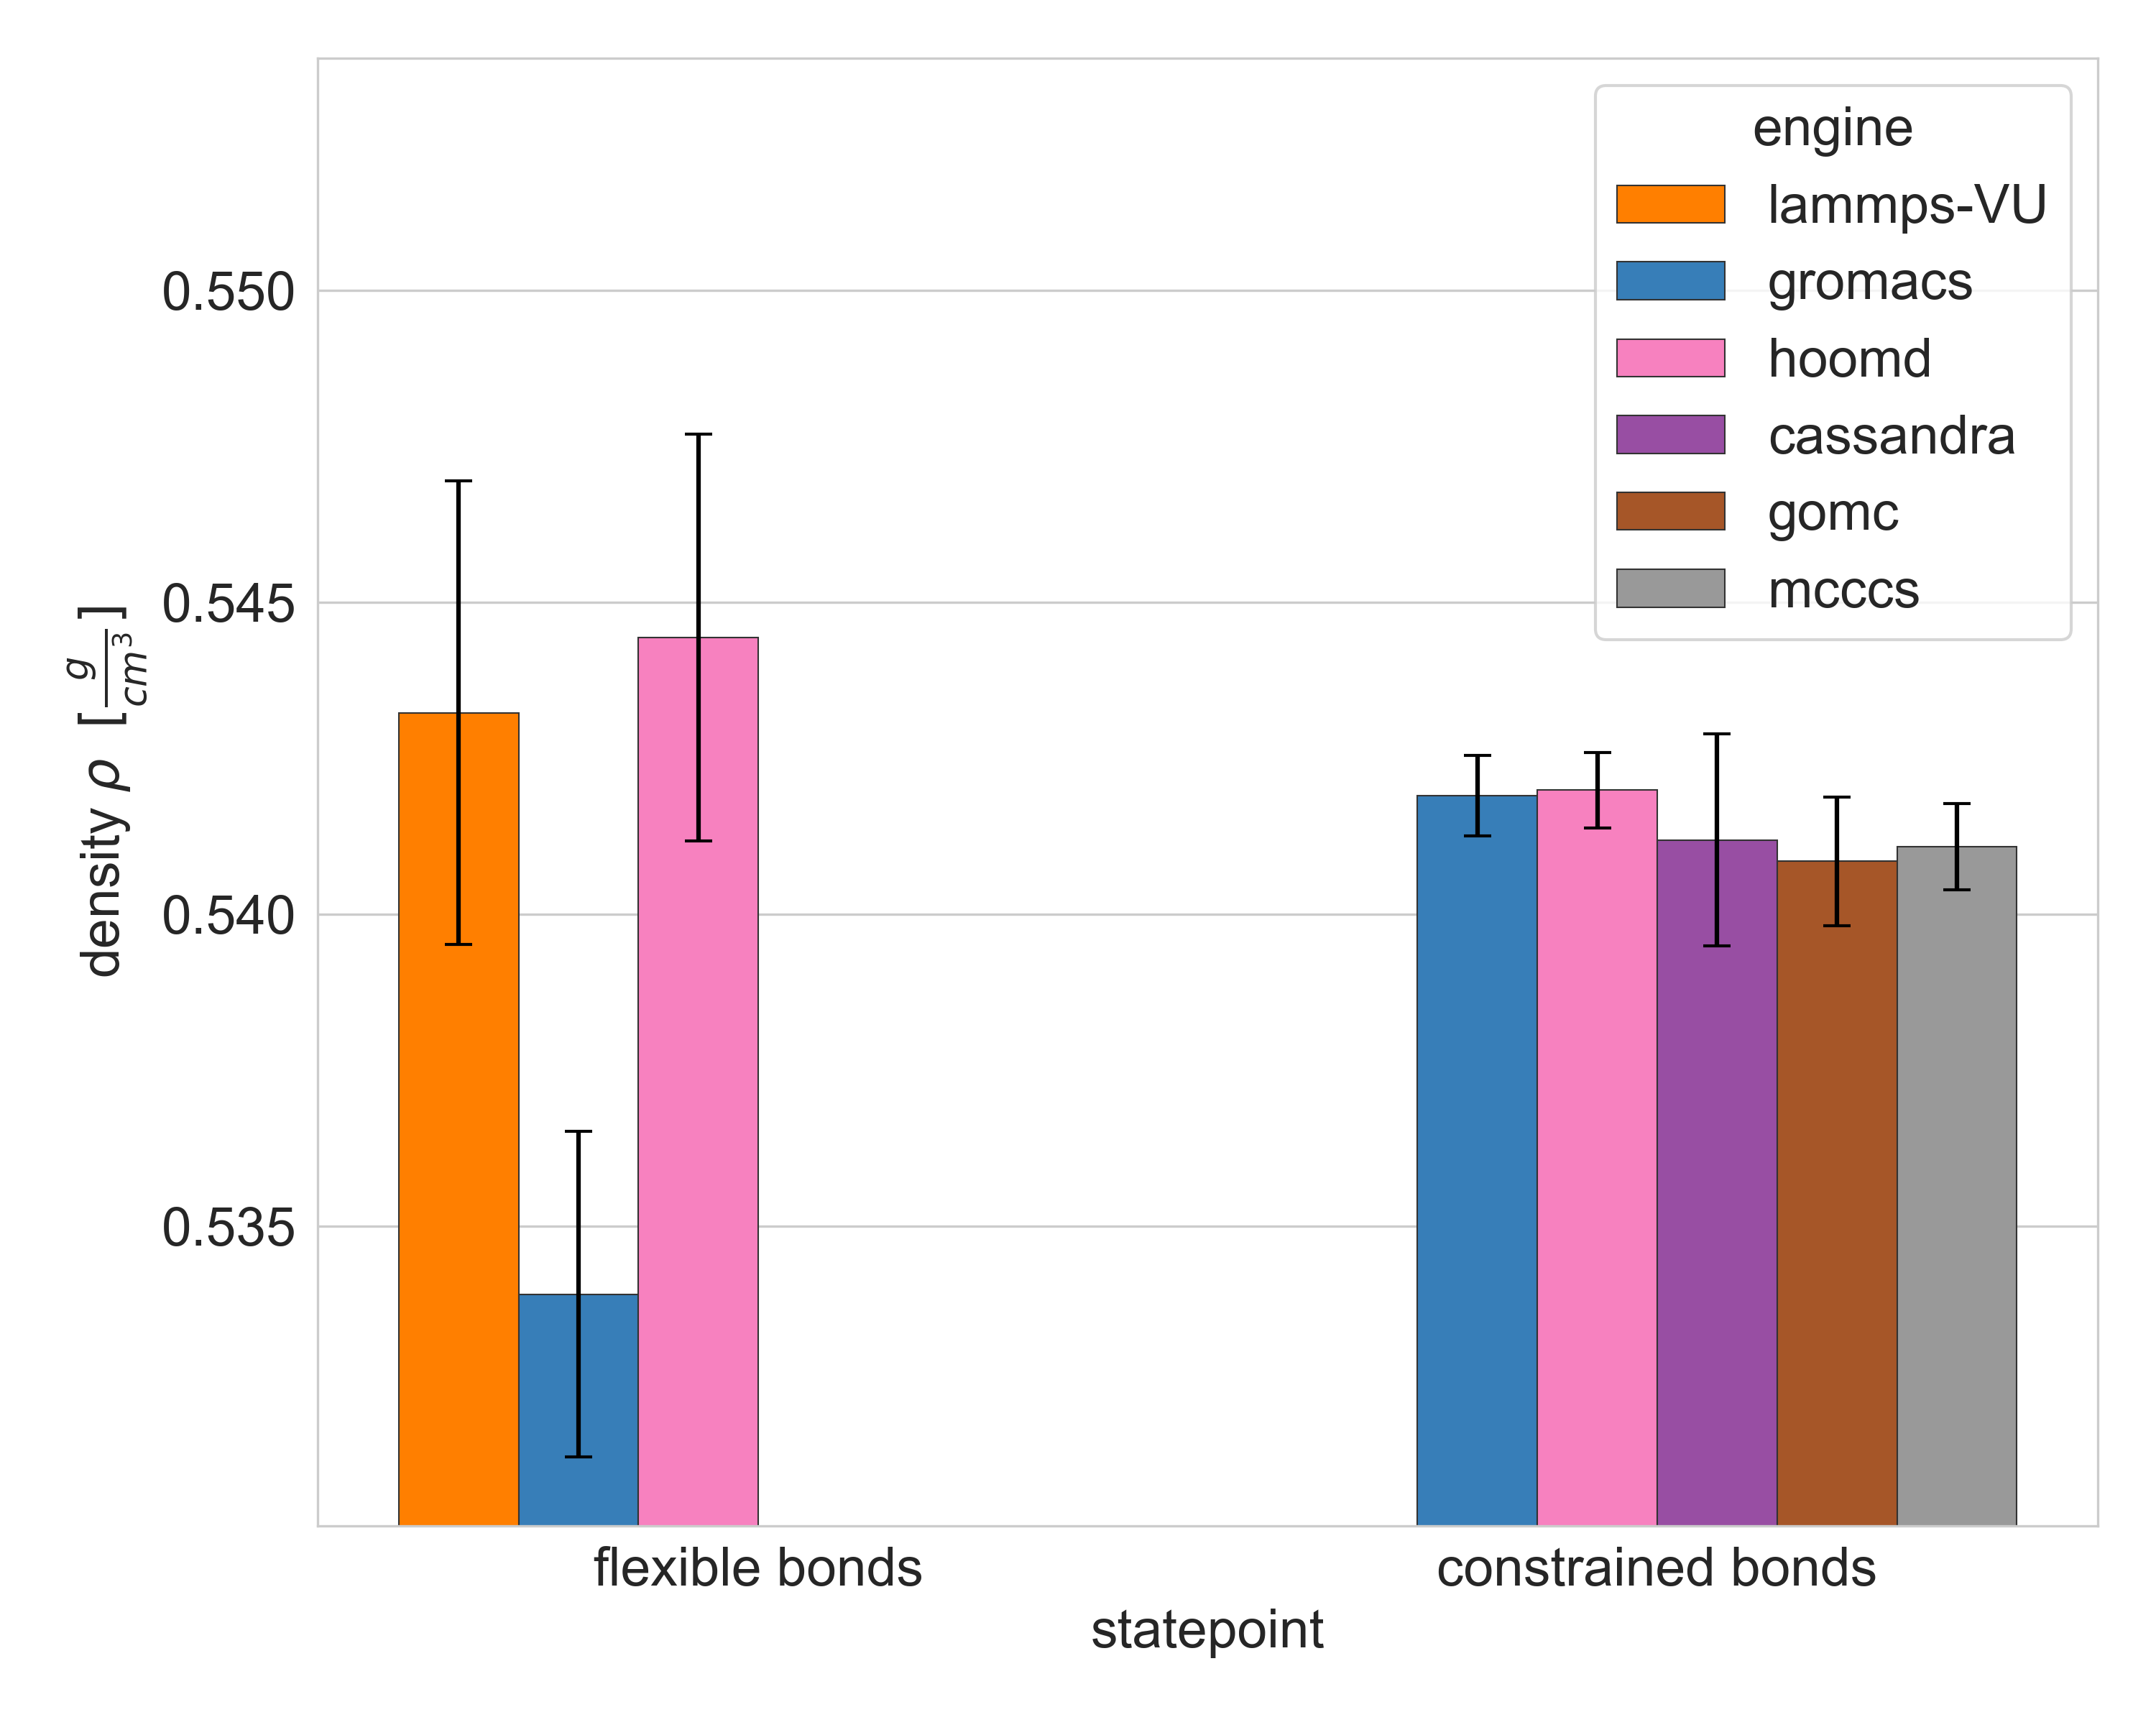
\includegraphics[width=0.6\linewidth,keepaspectratio]{figures/rep_study/pentane_summary.png}
    \caption{Average density of pentane with flexible or constrained bonds by engine. The average is taken from independent samples of the equilibrated regions of 16 replicates. The error bars represent two standard deviations in each direction.}\label{fig:pentane_density}
\end{figure}
I do not yet have data for constrained bond from LAMMPS, and so the only engines we can compare at this point are GROMACS and HOOMD.
Both engines seem to have greater variability in the density when using flexible bonds. 
This seems reasonable: allowing the bond lengths to fluctuate essentially allows the volume the molecule occupies to also fluctuate, so in order to keep the intermolecular forces consistent, the box volume must also fluctuate.
The HOOMD flexible and constrained bond pentane densities appear to agree within error although the density of the flexible bond pentane is higher.
For the GROMACS, however, the flexible pentane is much lower density and not within error of the constrained bond model.
Further investigation into the cause of this will be required.
The differences between the potential energy of the flexible and constrained bond pentane (see \autoref{fig:pentane_pe}) are much more clear.
\begin{figure}[h!]
    \centering
    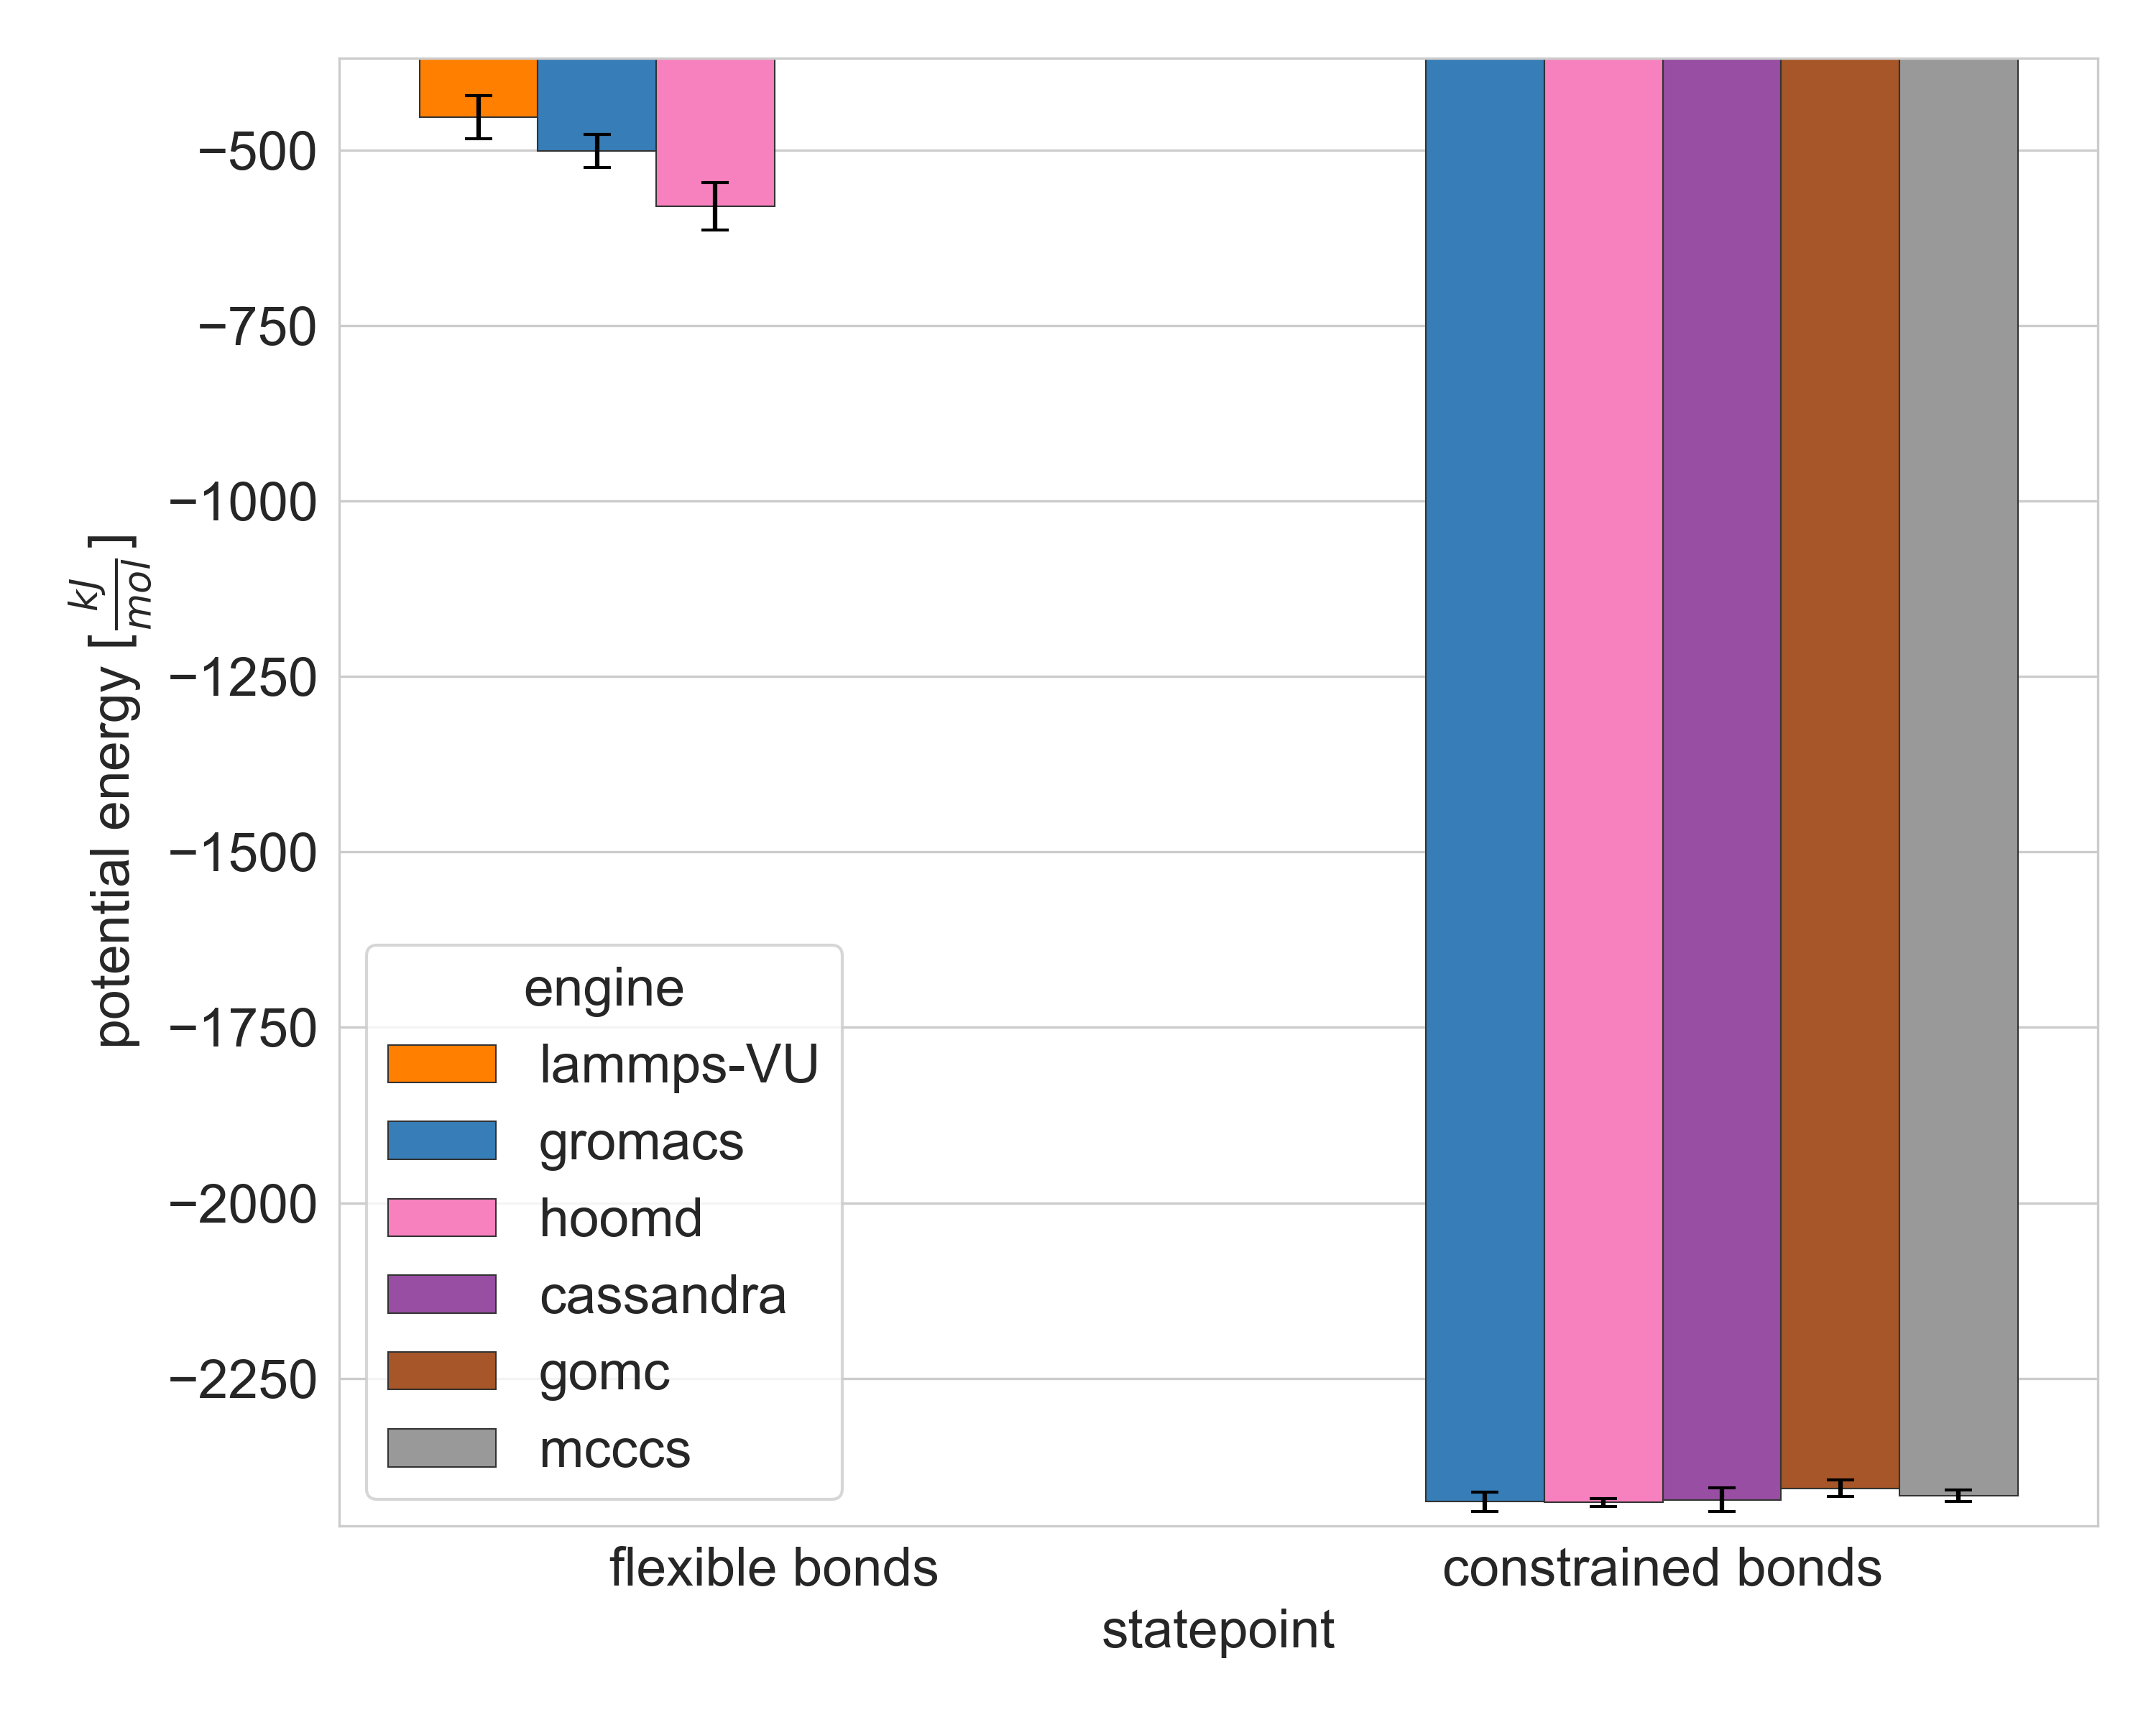
\includegraphics[width=0.6\linewidth,keepaspectratio]{figures/rep_study/pentane_pe_summary.png}
    \caption{Average potential energy of pentane by engine. The average is taken from independent samples of the equilibrated regions of 16 replicates. The error bars represent two standard deviations in each direction.}\label{fig:pentane_pe}
\end{figure}
The potential energies for the constrained bond pentane are much lower because the bond lengths for all systems are fixed at their equilibrium length, which is the minima of the harmonic bond potential.
In the flexible bond model, the bond is allowed to deviate from its equilibrium length, resulting in higher positive contribution to potential energy from the bond. 
This difference will be seen in the potential energies for other systems. 
When the bond lengths are fixed (as in the water and benzene models), the potential energy values observed by MD are closer to those observed by MC. 
(A direct comparison of flexible vs fixed bonds is shown in \autoref{fig:pentane_pe}, but \autoref{fig:water_pe} and \autoref{fig:benzene_pe} also are rigid models or have fixed bonds.)

\begin{figure}[h!]
    \centering
    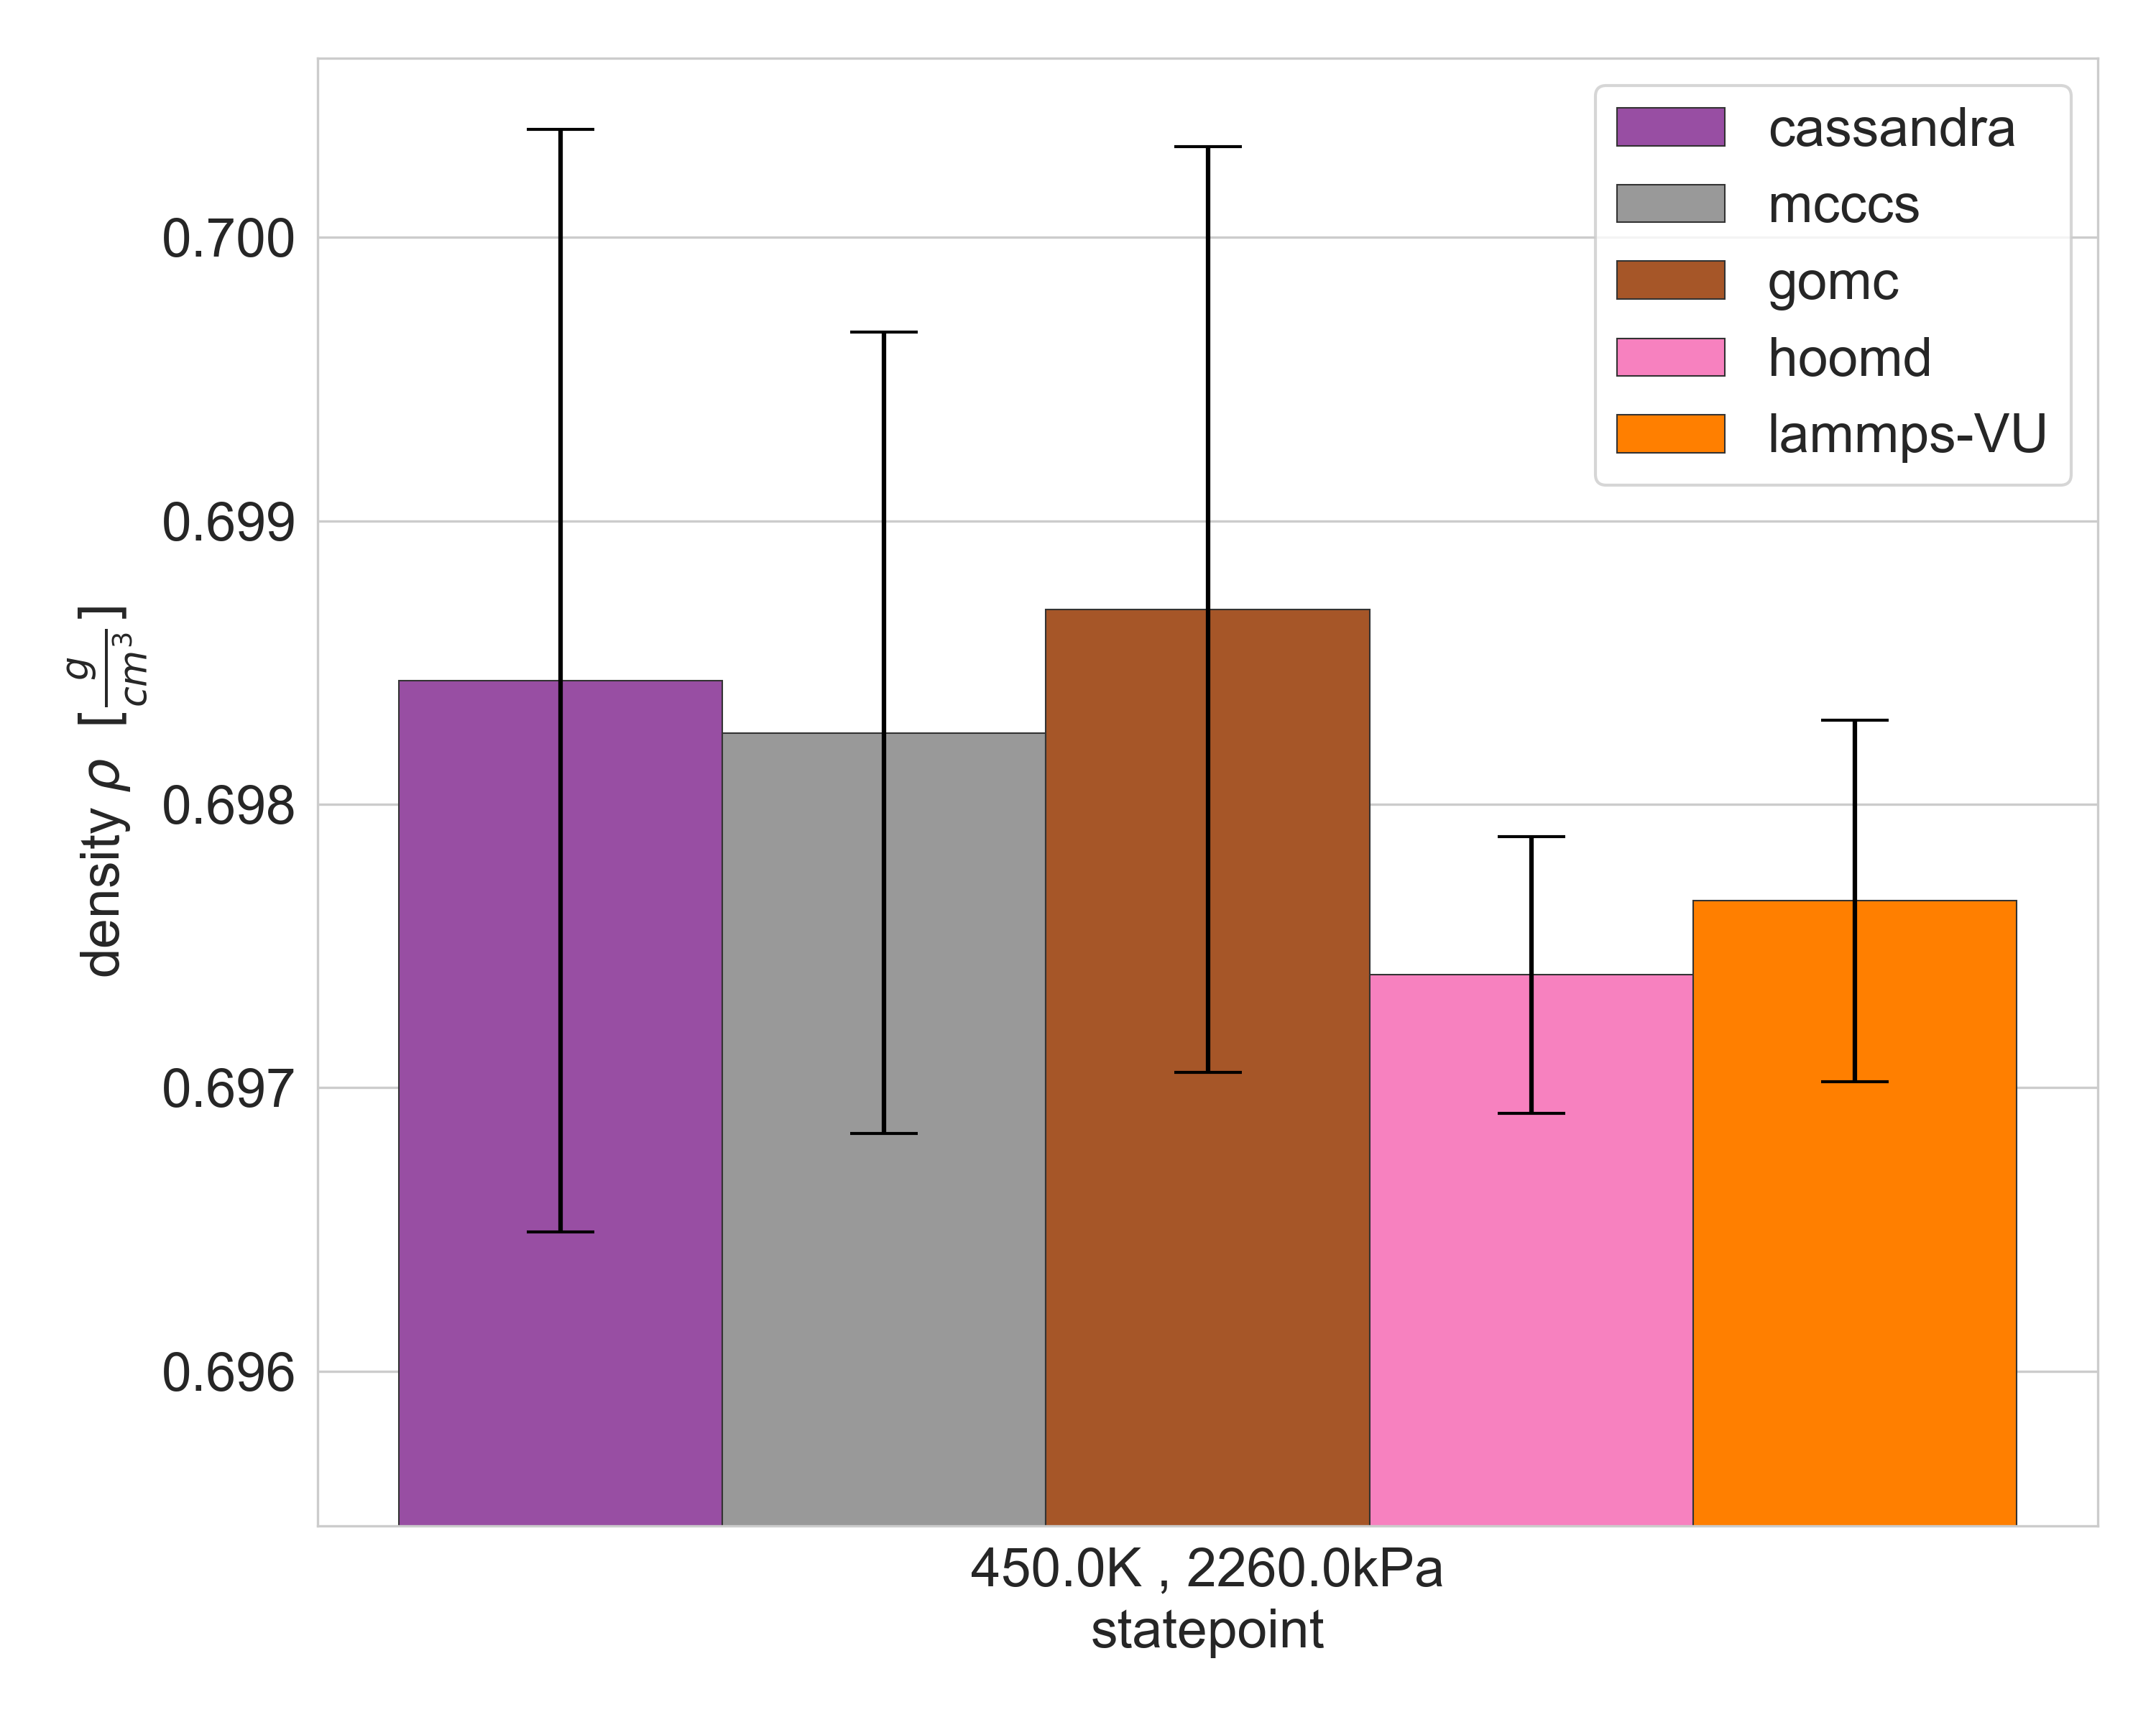
\includegraphics[width=0.6\linewidth,keepaspectratio]{figures/rep_study/benzeneUA_summary.png}
    \caption{Average density of benzene by engine. The average is taken from independent samples of the equilibrated regions of 16 replicates. The error bars represent two standard deviations in each direction.}\label{fig:benzene_density}
\end{figure}
Next, let's examine UA benzene, which is a ring structure modelled as a rigid body. 
I will use the term "rigid body", although the actual implementation may vary depending on the options available in each engine.
Some engines may be fixing bonds, angles, and dihedrals, while others (like HOOMD) may support true rigid bodies.
Although the implementations of rigidness may differ between engines, the average density of benzene between engines agrees within error (see \autoref{fig:benzene_density}).
Again we see slightly lower density with greater variation in MC, the reasons for this are likely the same as with methane. % should I even say this?
\autoref{fig:benzene_pe} shows the potential energies of benzene by engine.
\begin{figure}[h!]
    \centering
    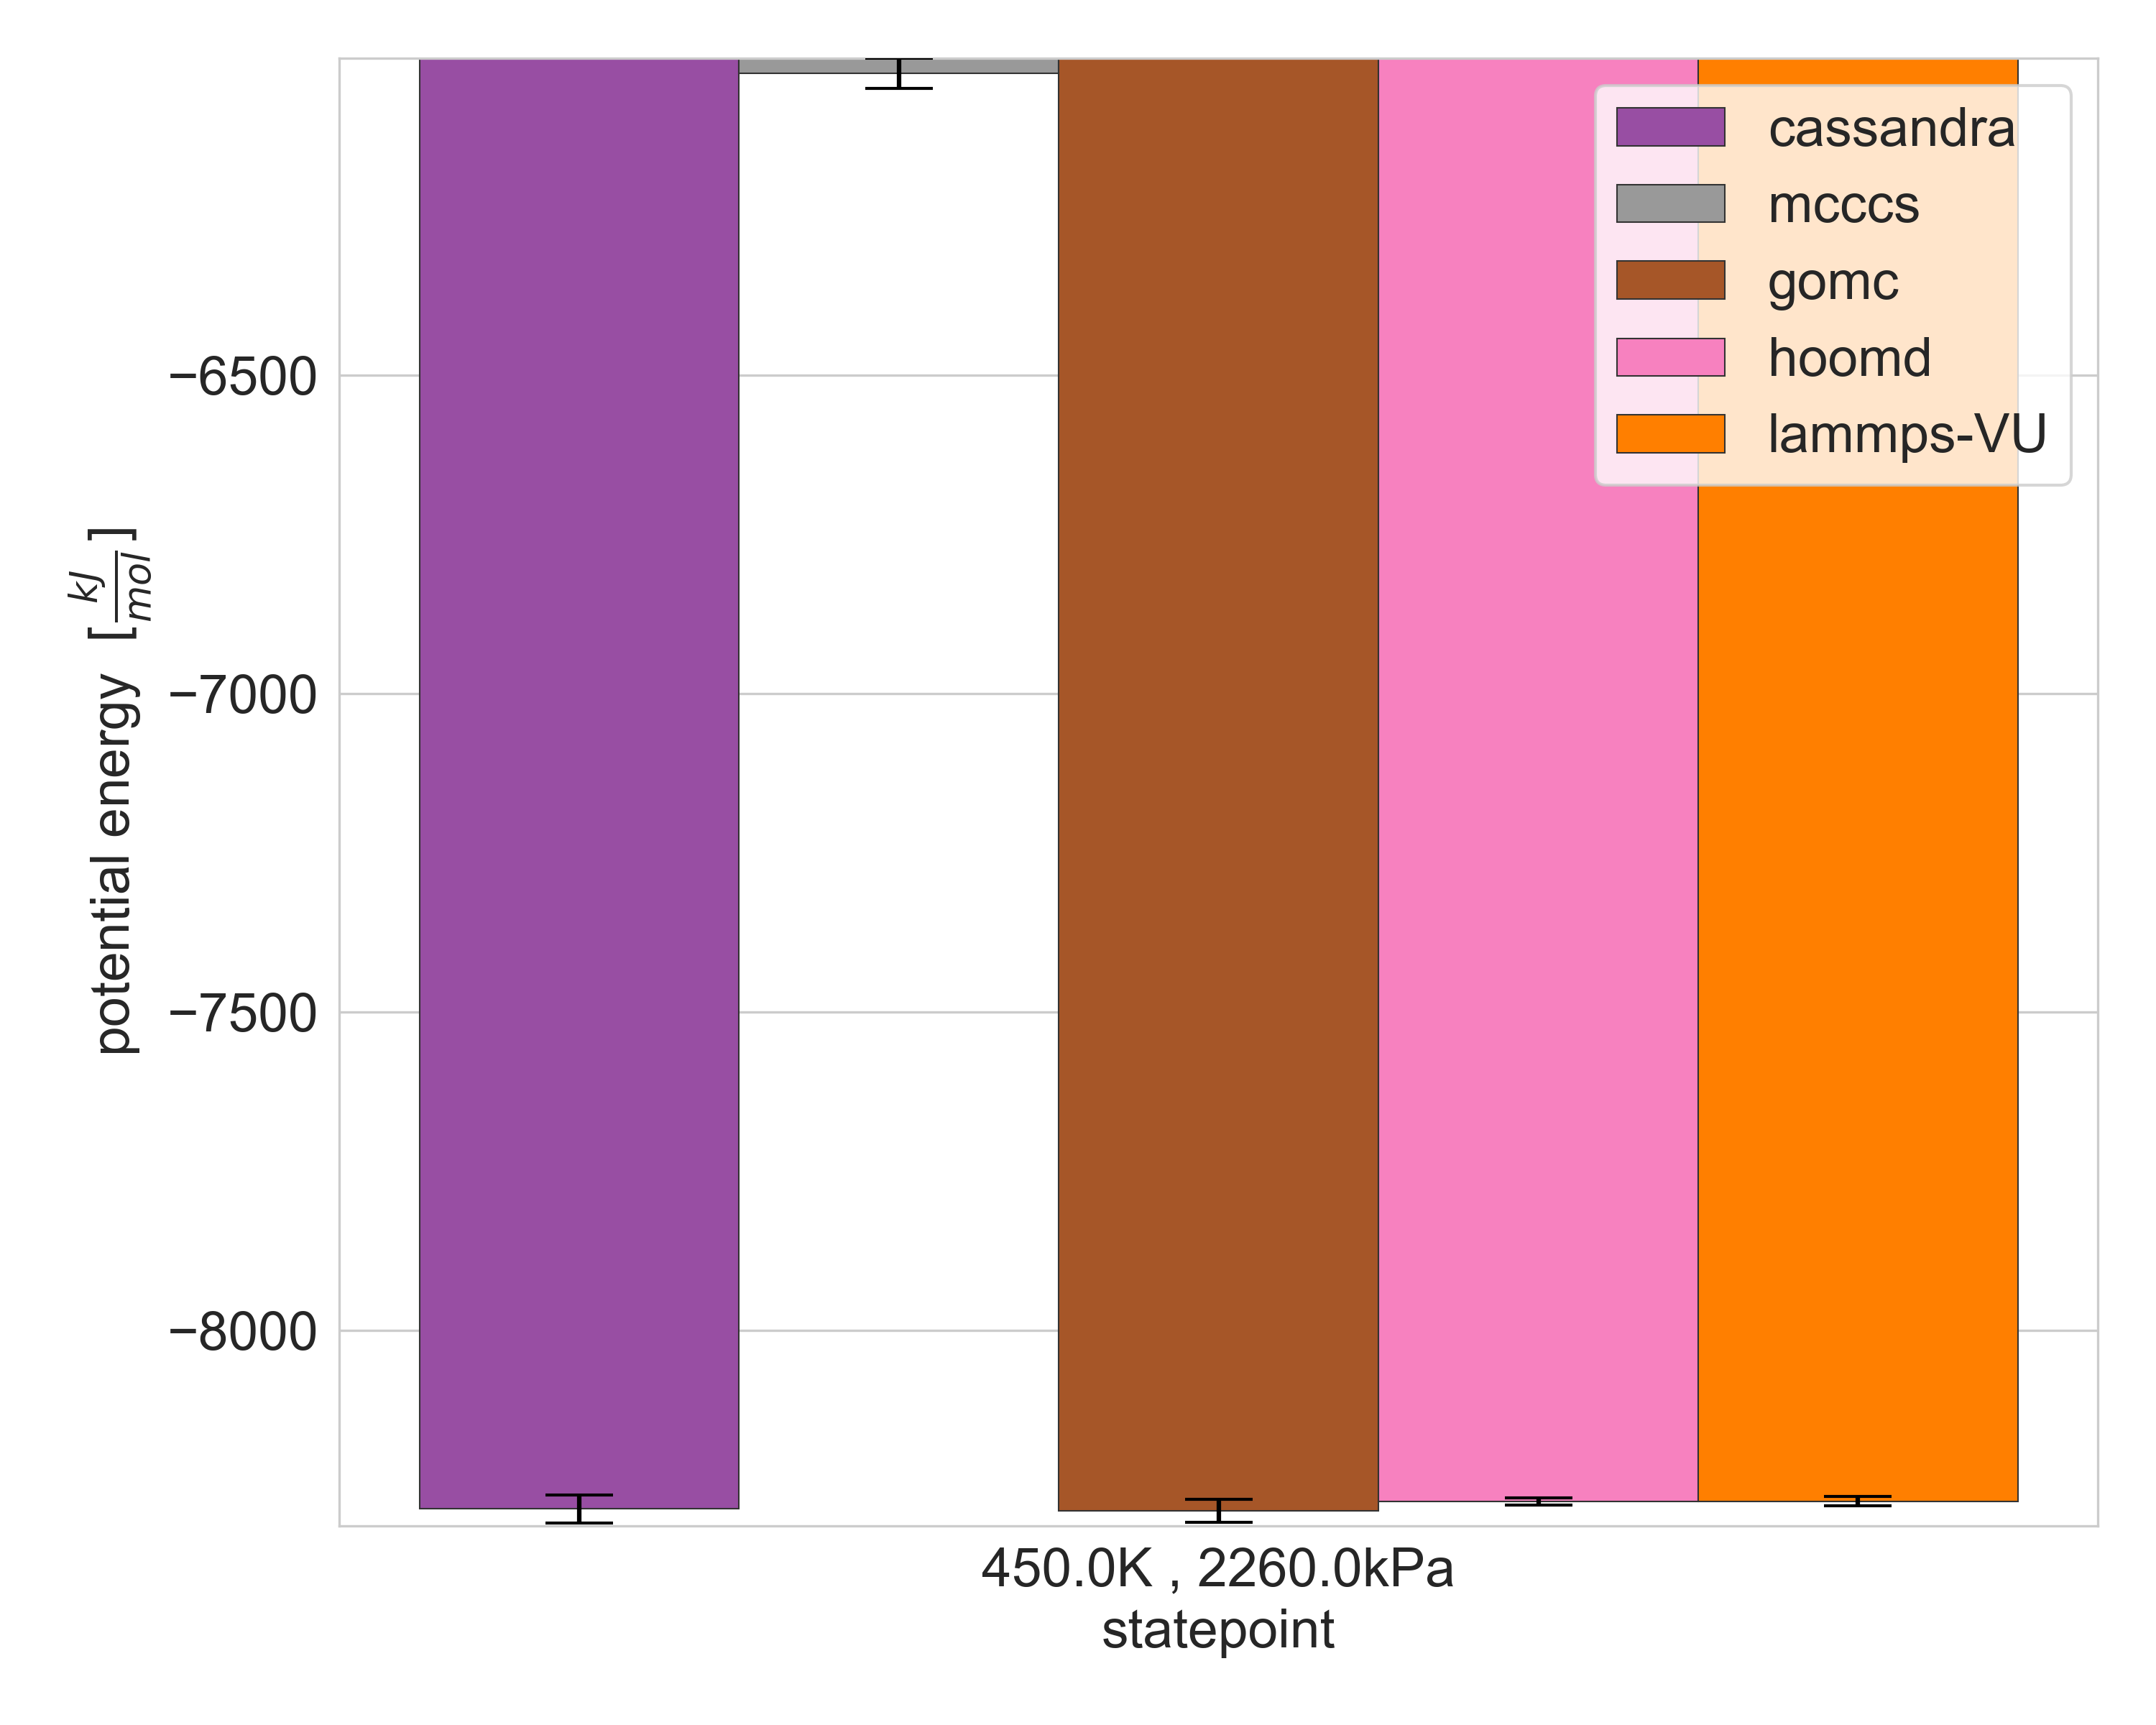
\includegraphics[width=0.6\linewidth,keepaspectratio]{figures/rep_study/benzeneUA_pe_summary.png}
    \caption{Average potential energy of benzene by engine. The average is taken from independent samples of the equilibrated regions of 16 replicates. The error bars represent two standard deviations in each direction.}\label{fig:benzene_pe}
\end{figure}
With the exception of MCCCS, the potential energies agree within error. 
Further investigation will be required into the incongruous energy value reported by MCCCS.

Next, let's examine SPC/E water, which is modelled as a rigid three-site charged molecule. 
\autoref{fig:water_density} shows the density of water by engines at three statepoints.
\begin{figure}[h!]
    \centering
    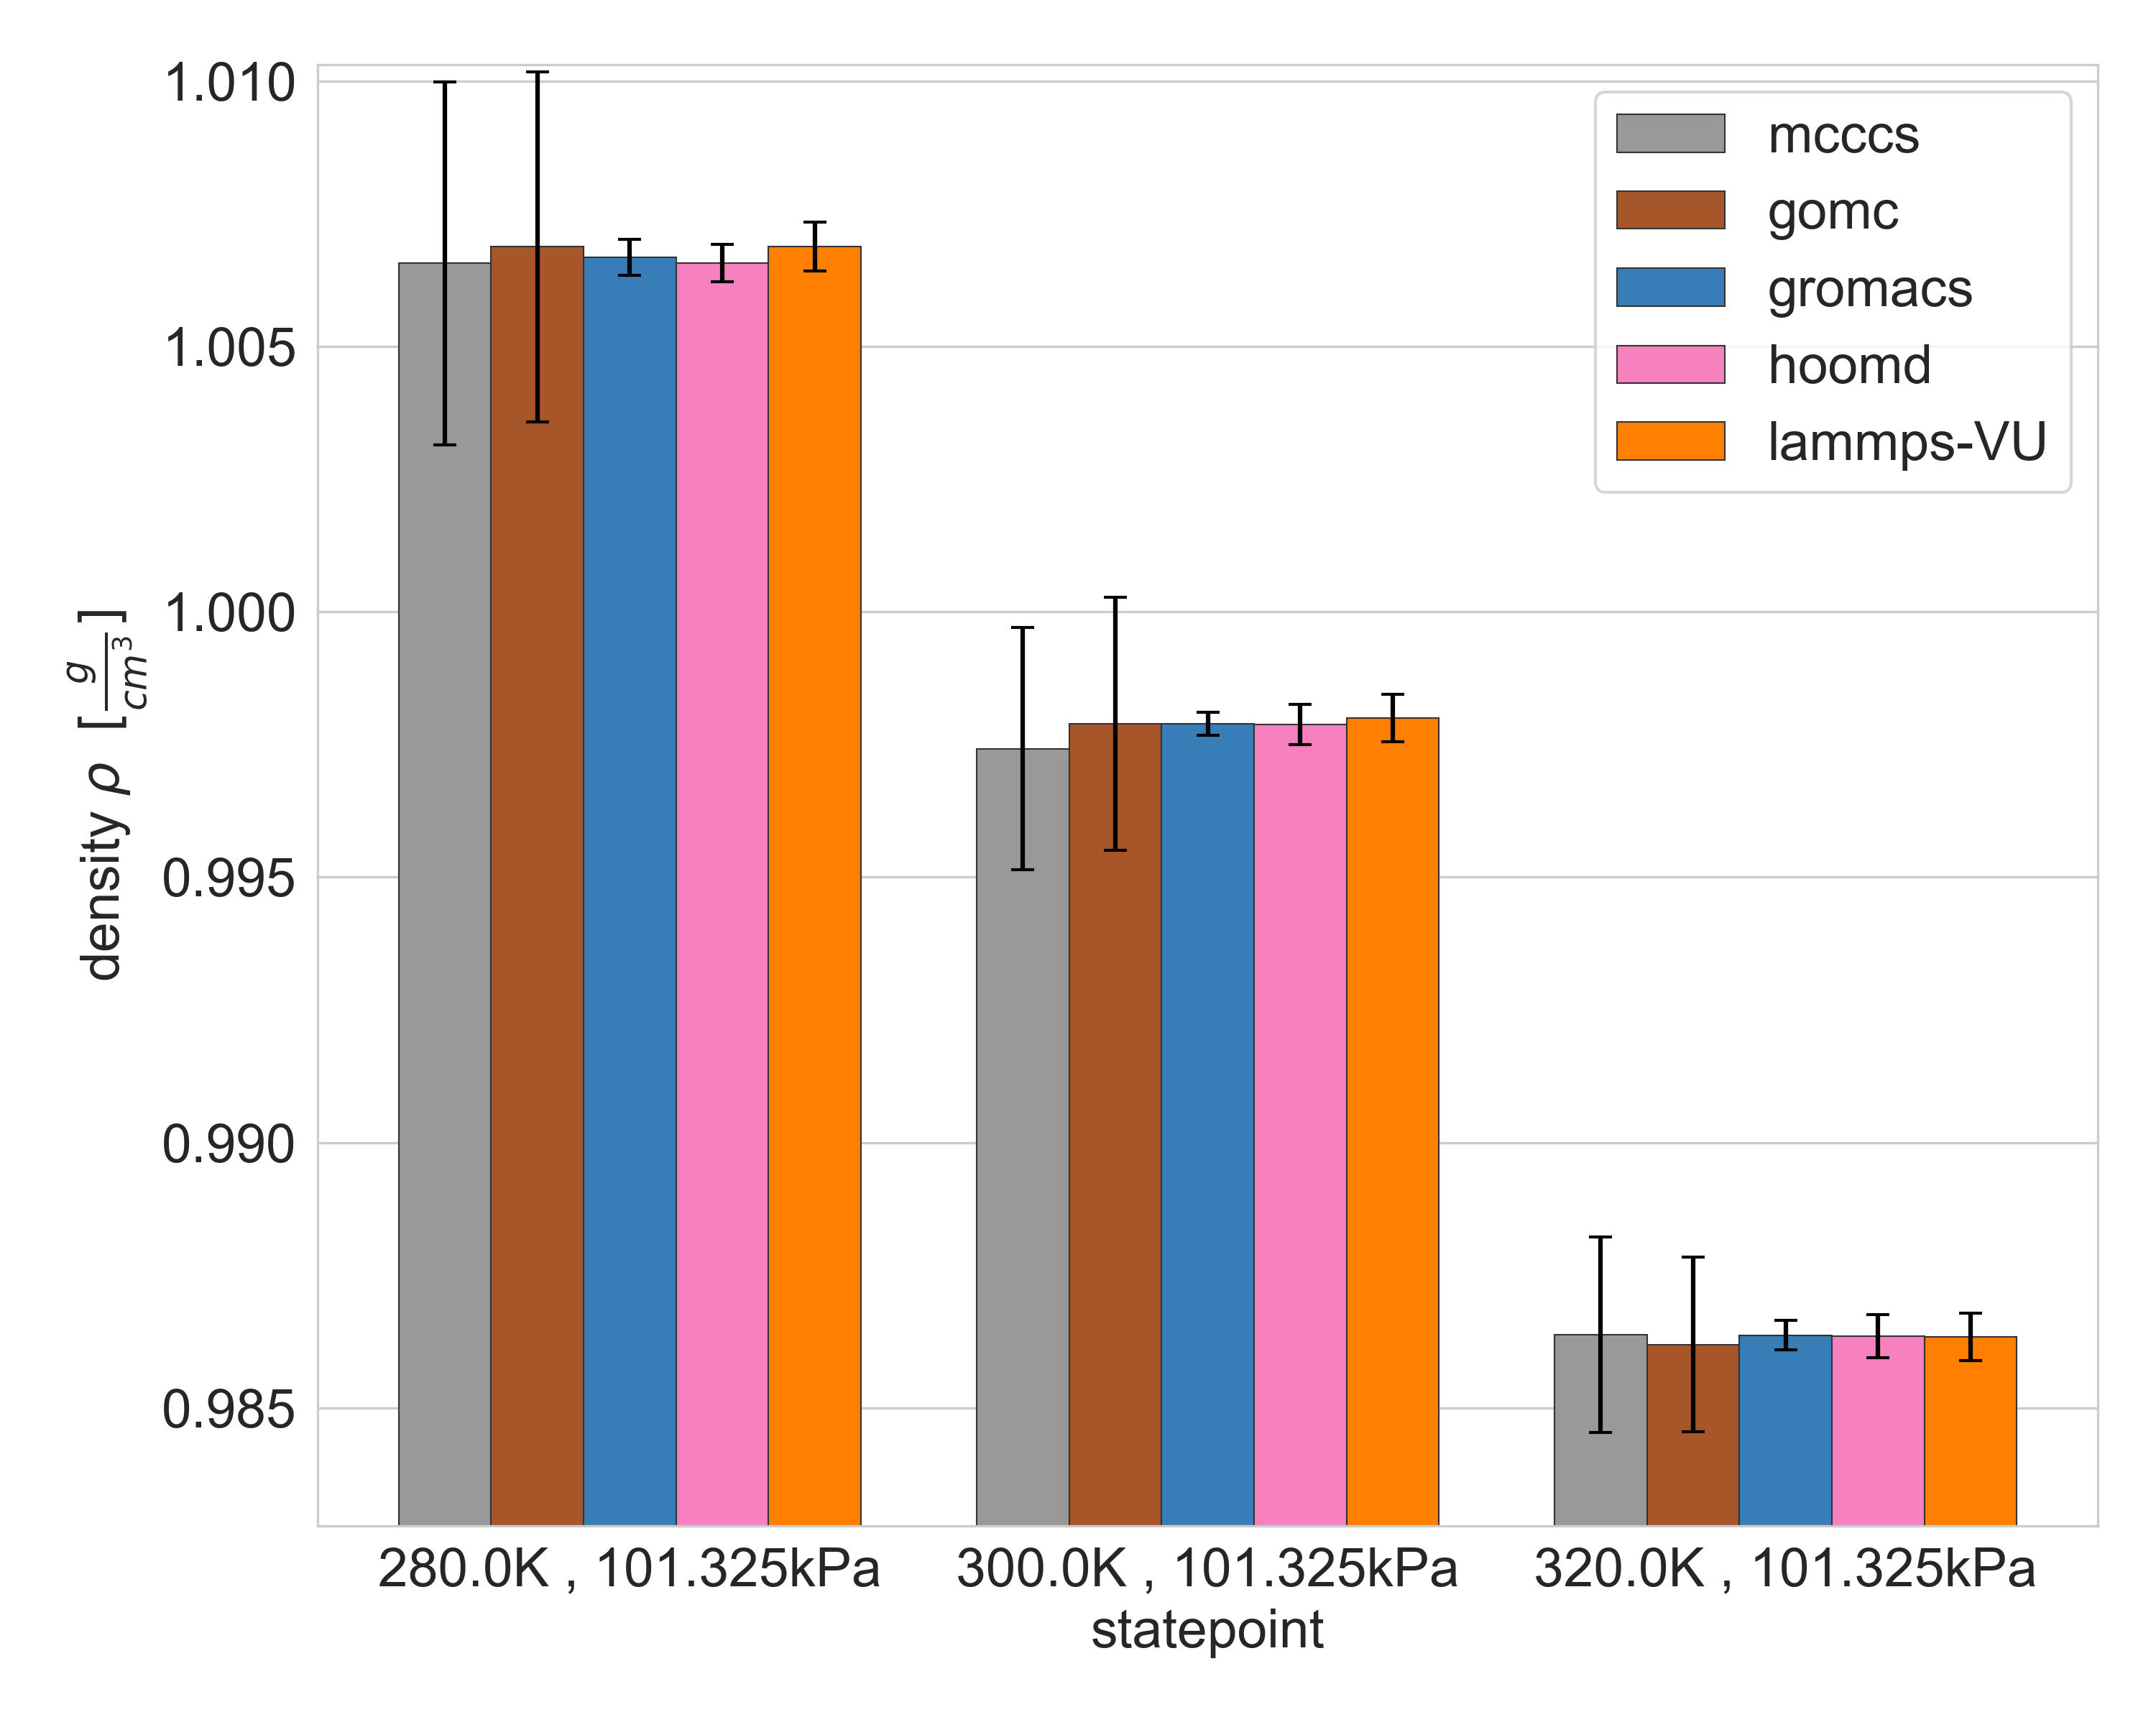
\includegraphics[width=0.6\linewidth,keepaspectratio]{figures/rep_study/waterSPCE_summary.png}
    \caption{Average density of water at three statepoints by engine. The average is taken from independent samples of the equilibrated regions of 16 replicates. The error bars represent two standard deviations in each direction.}\label{fig:water_density}
\end{figure}
The density of water at each statepoint appears to agree within error between all engines
The average densities are also relatively close to the predicted values: 0.99991, 0.99656, and 0.98953 g/cm$^3$, respectively \cite{NISTwebbook}.
The potential energies of water at these three statepoints \autoref{fig:water_pe} show similar agreement with the exception of LAMMPS.
\begin{figure}[h!]
    \centering
    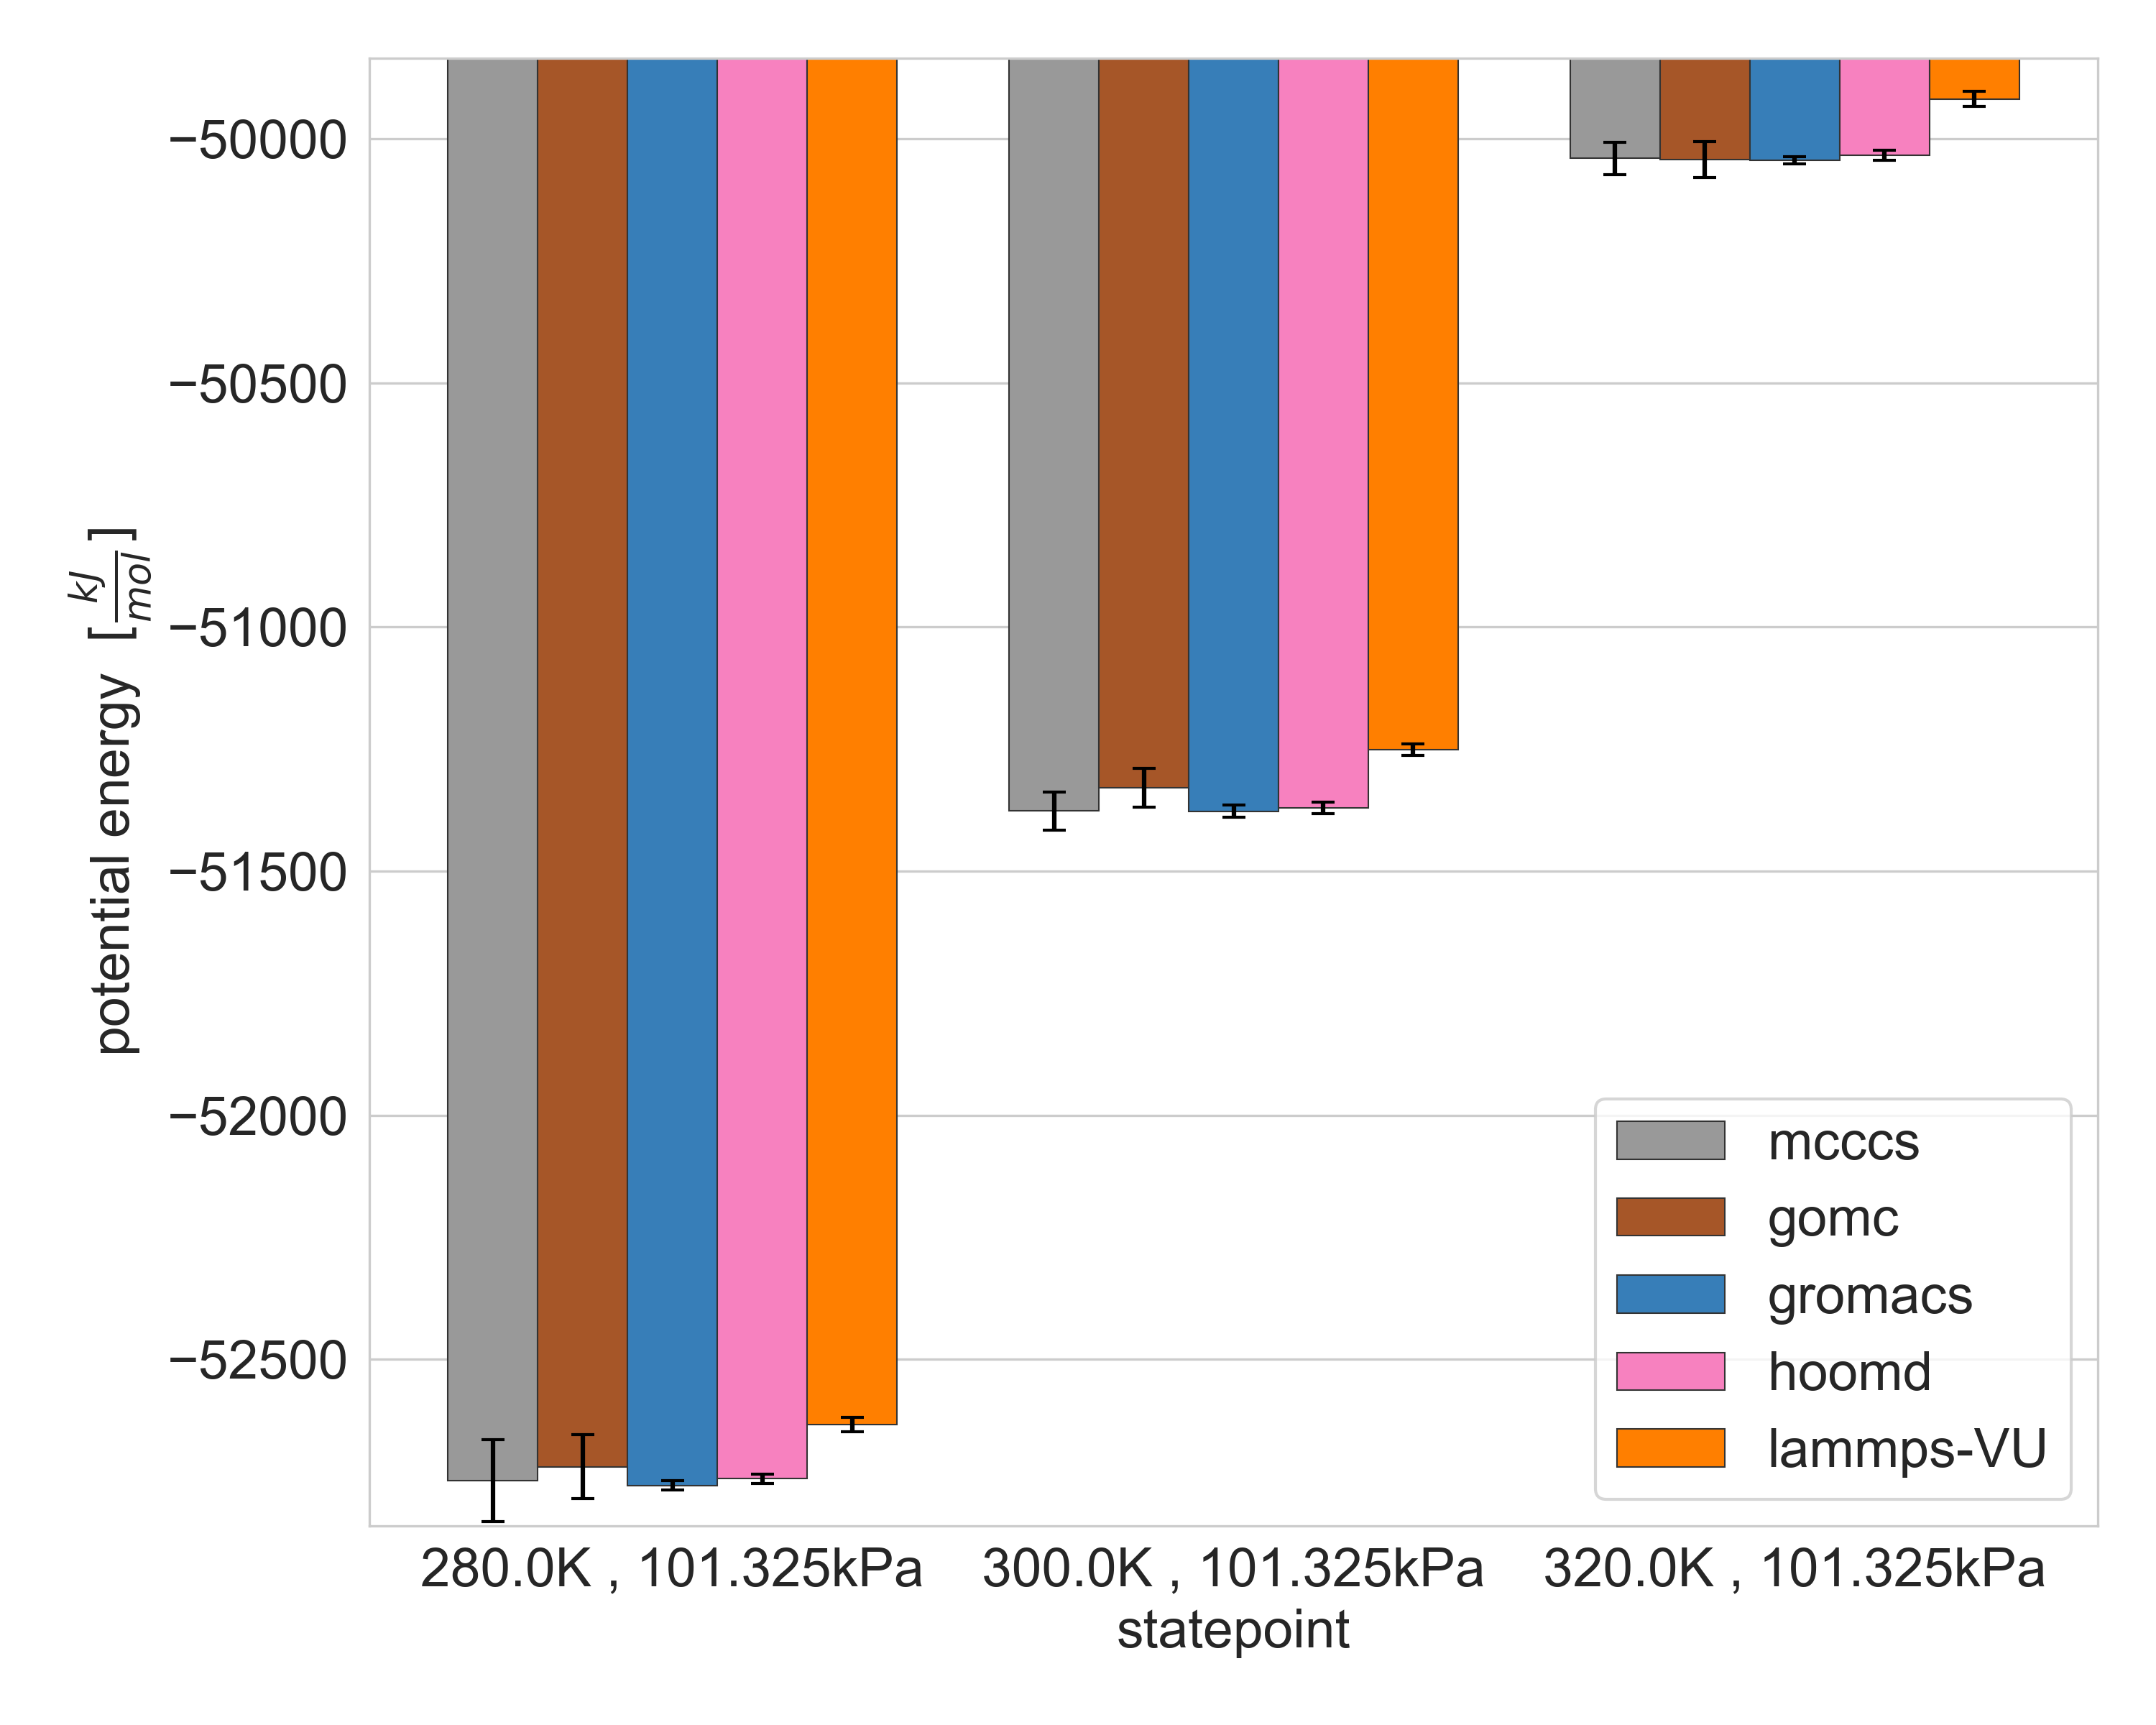
\includegraphics[width=0.6\linewidth,keepaspectratio]{figures/rep_study/waterSPCE_pe_summary.png}
    \caption{Average potential energy of water by engine. The average is taken from independent samples of the equilibrated regions of 16 replicates. The error bars represent two standard deviations in each direction.}\label{fig:water_pe}
\end{figure}
It seems that this discrepancy is related to the PPPM implementation in LAMMPS because the potential energy is systematically high in both charged systems (see \autoref{fig:water_pe} and \autoref{fig:ethanol_pe}).
Further investigation into this discrepancy will be required.

Finally, let's look at the most complex system, all-atom ethanol, which is a fully-flexible molecule with charges.
(Full flexibility, of course, depends on the engine's capabilities, so MD engines modelled this system with flexible bonds and MC engines used fixed bonds.)
The densities of ethanol by engines at three statepoints is shown in \autoref{fig:ethanol_density}.
\begin{figure}[h!]
    \centering
    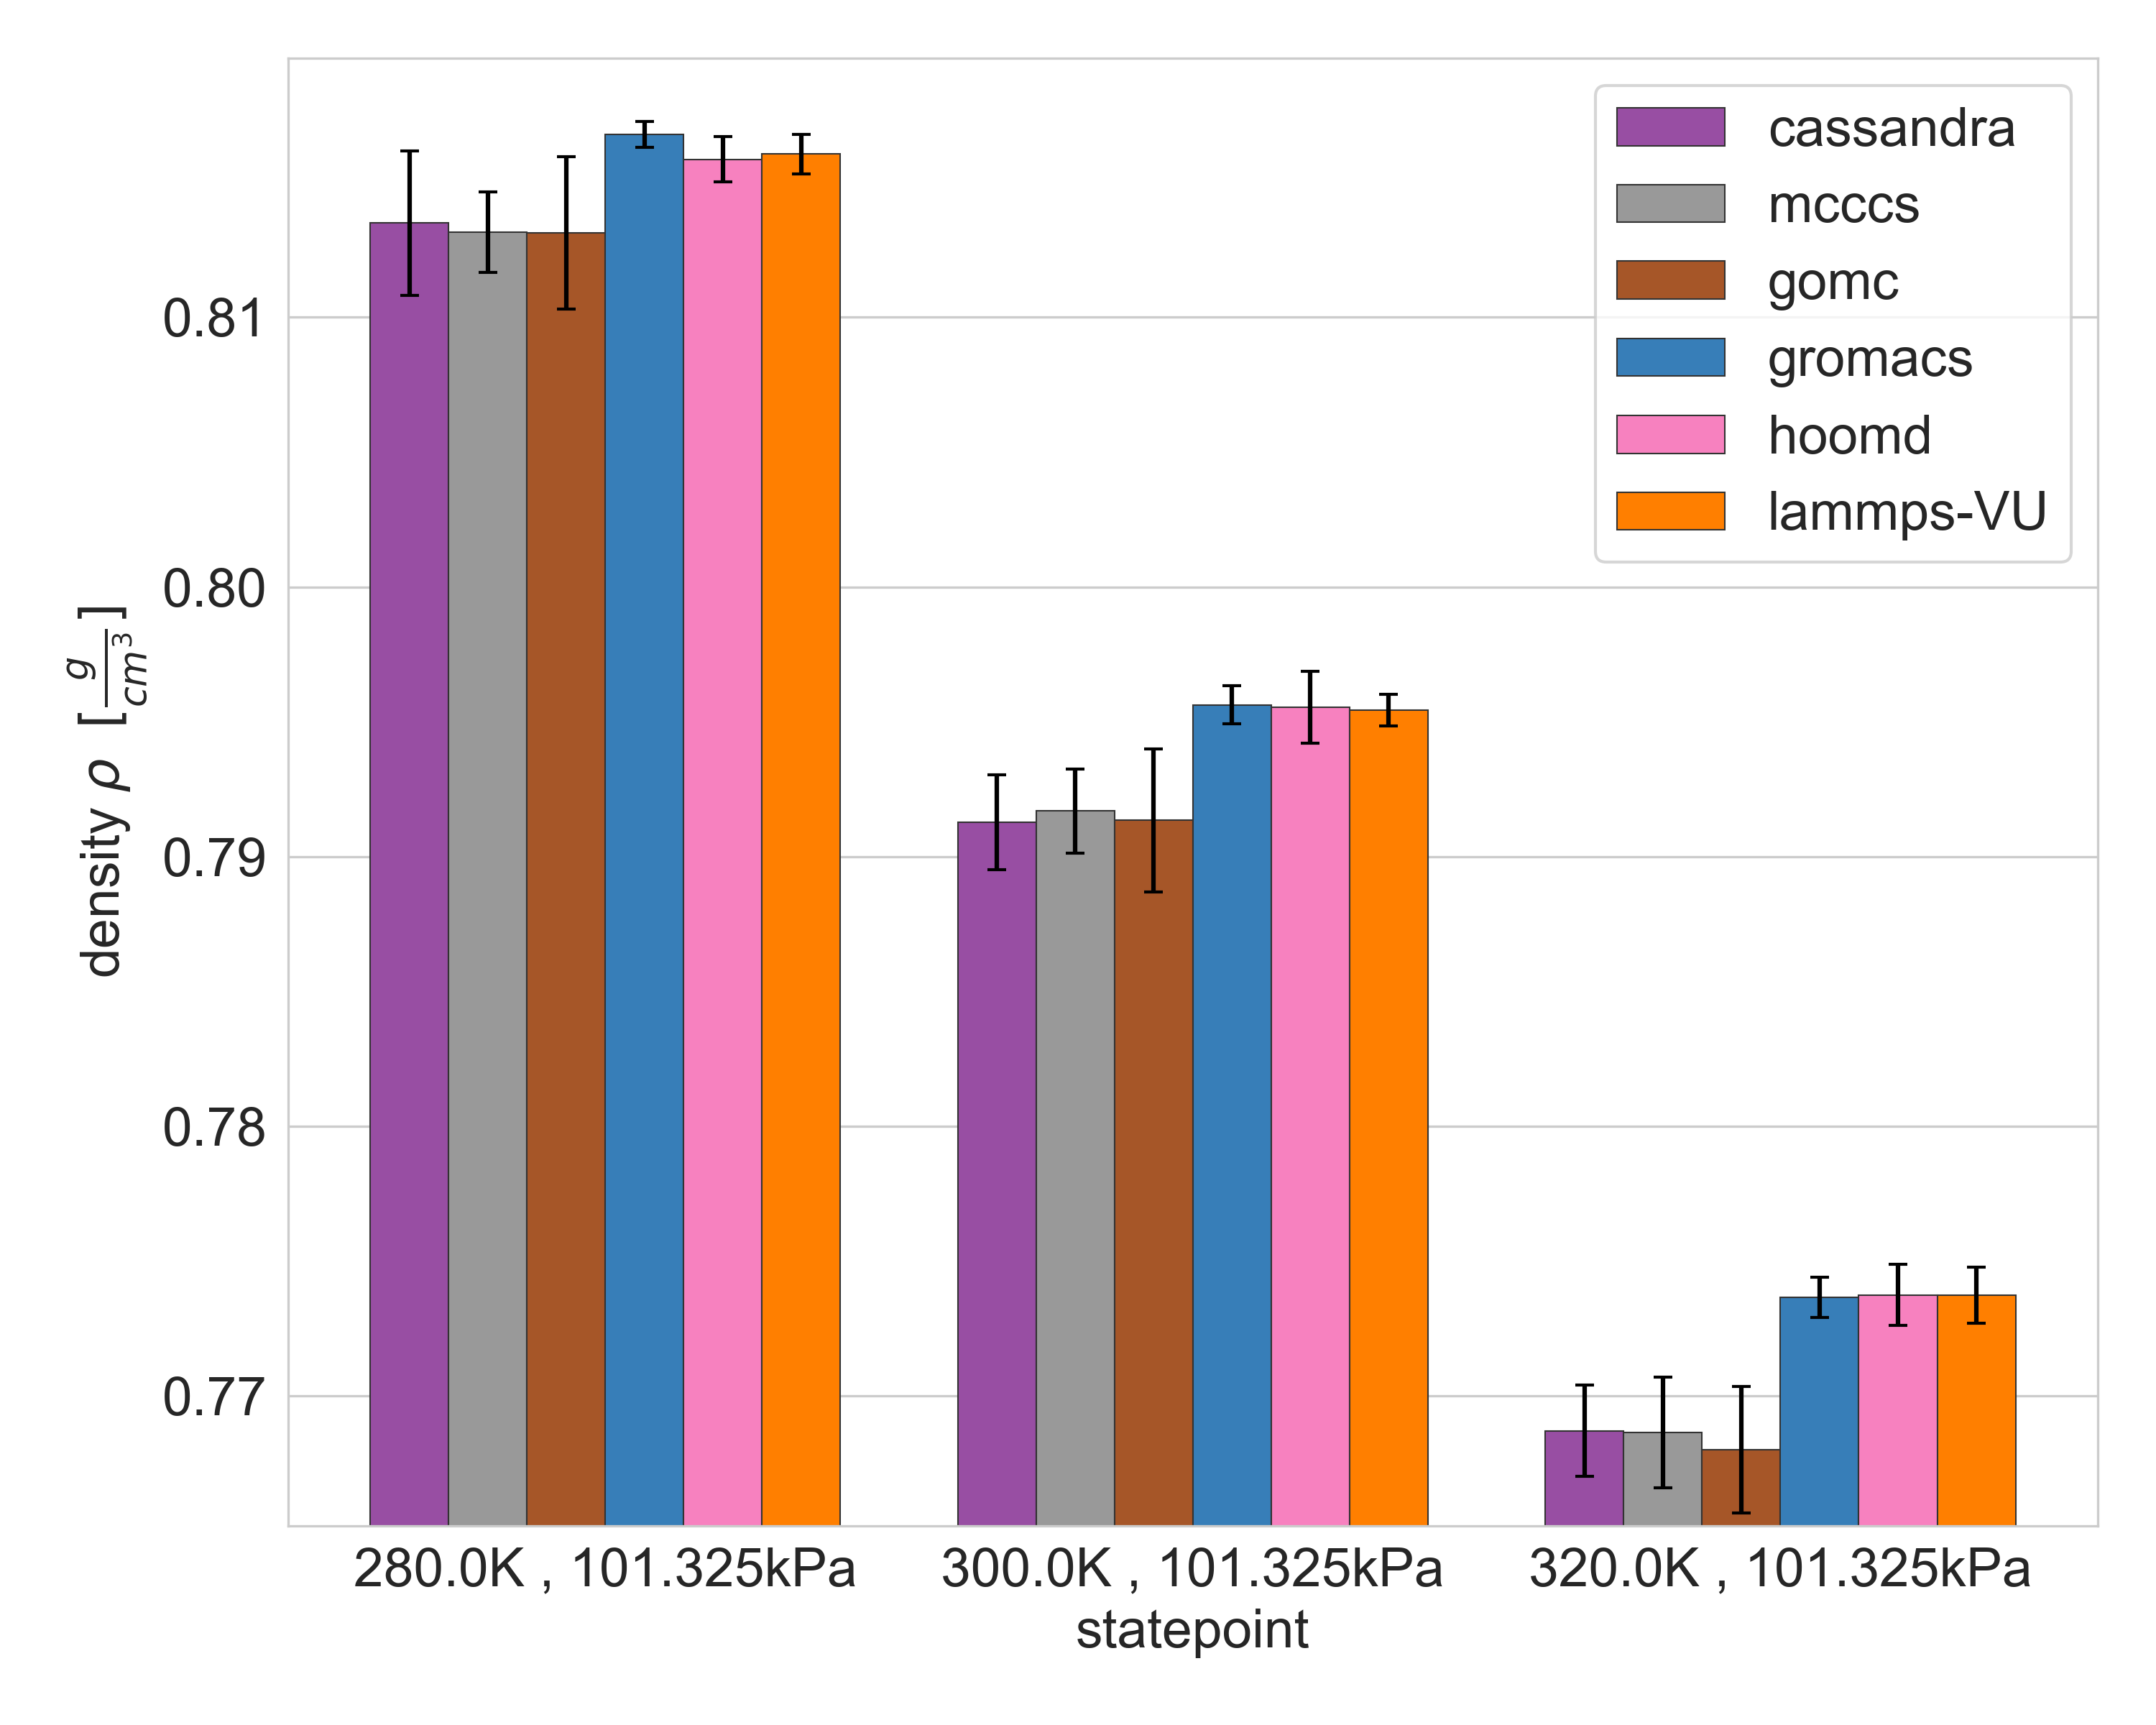
\includegraphics[width=0.6\linewidth,keepaspectratio]{figures/rep_study/ethanolAA_summary.png}
    \caption{Average density of ethanol by engine. The average is taken from independent samples of the equilibrated regions of 16 replicates. The error bars represent two standard deviations in each direction.}\label{fig:ethanol_density}
\end{figure}
The densities agree within error for each method (MC or MD), but this time the density observed in MD is higher than that in MC.
It is hard to make a clear statement for what is causing this discrepancy in densities between the two methods with the data available, but comparison with \autoref{fig:pentane_density} could suggest that the higher density observed in MD is due to the flexible bonds.
The potential energies of ethanol (see \autoref{fig:ethanol_pe}) show the greatest variability between engines; however, this can be attributed to two issues which have already been discussed.
\begin{figure}[h!]
    \centering
    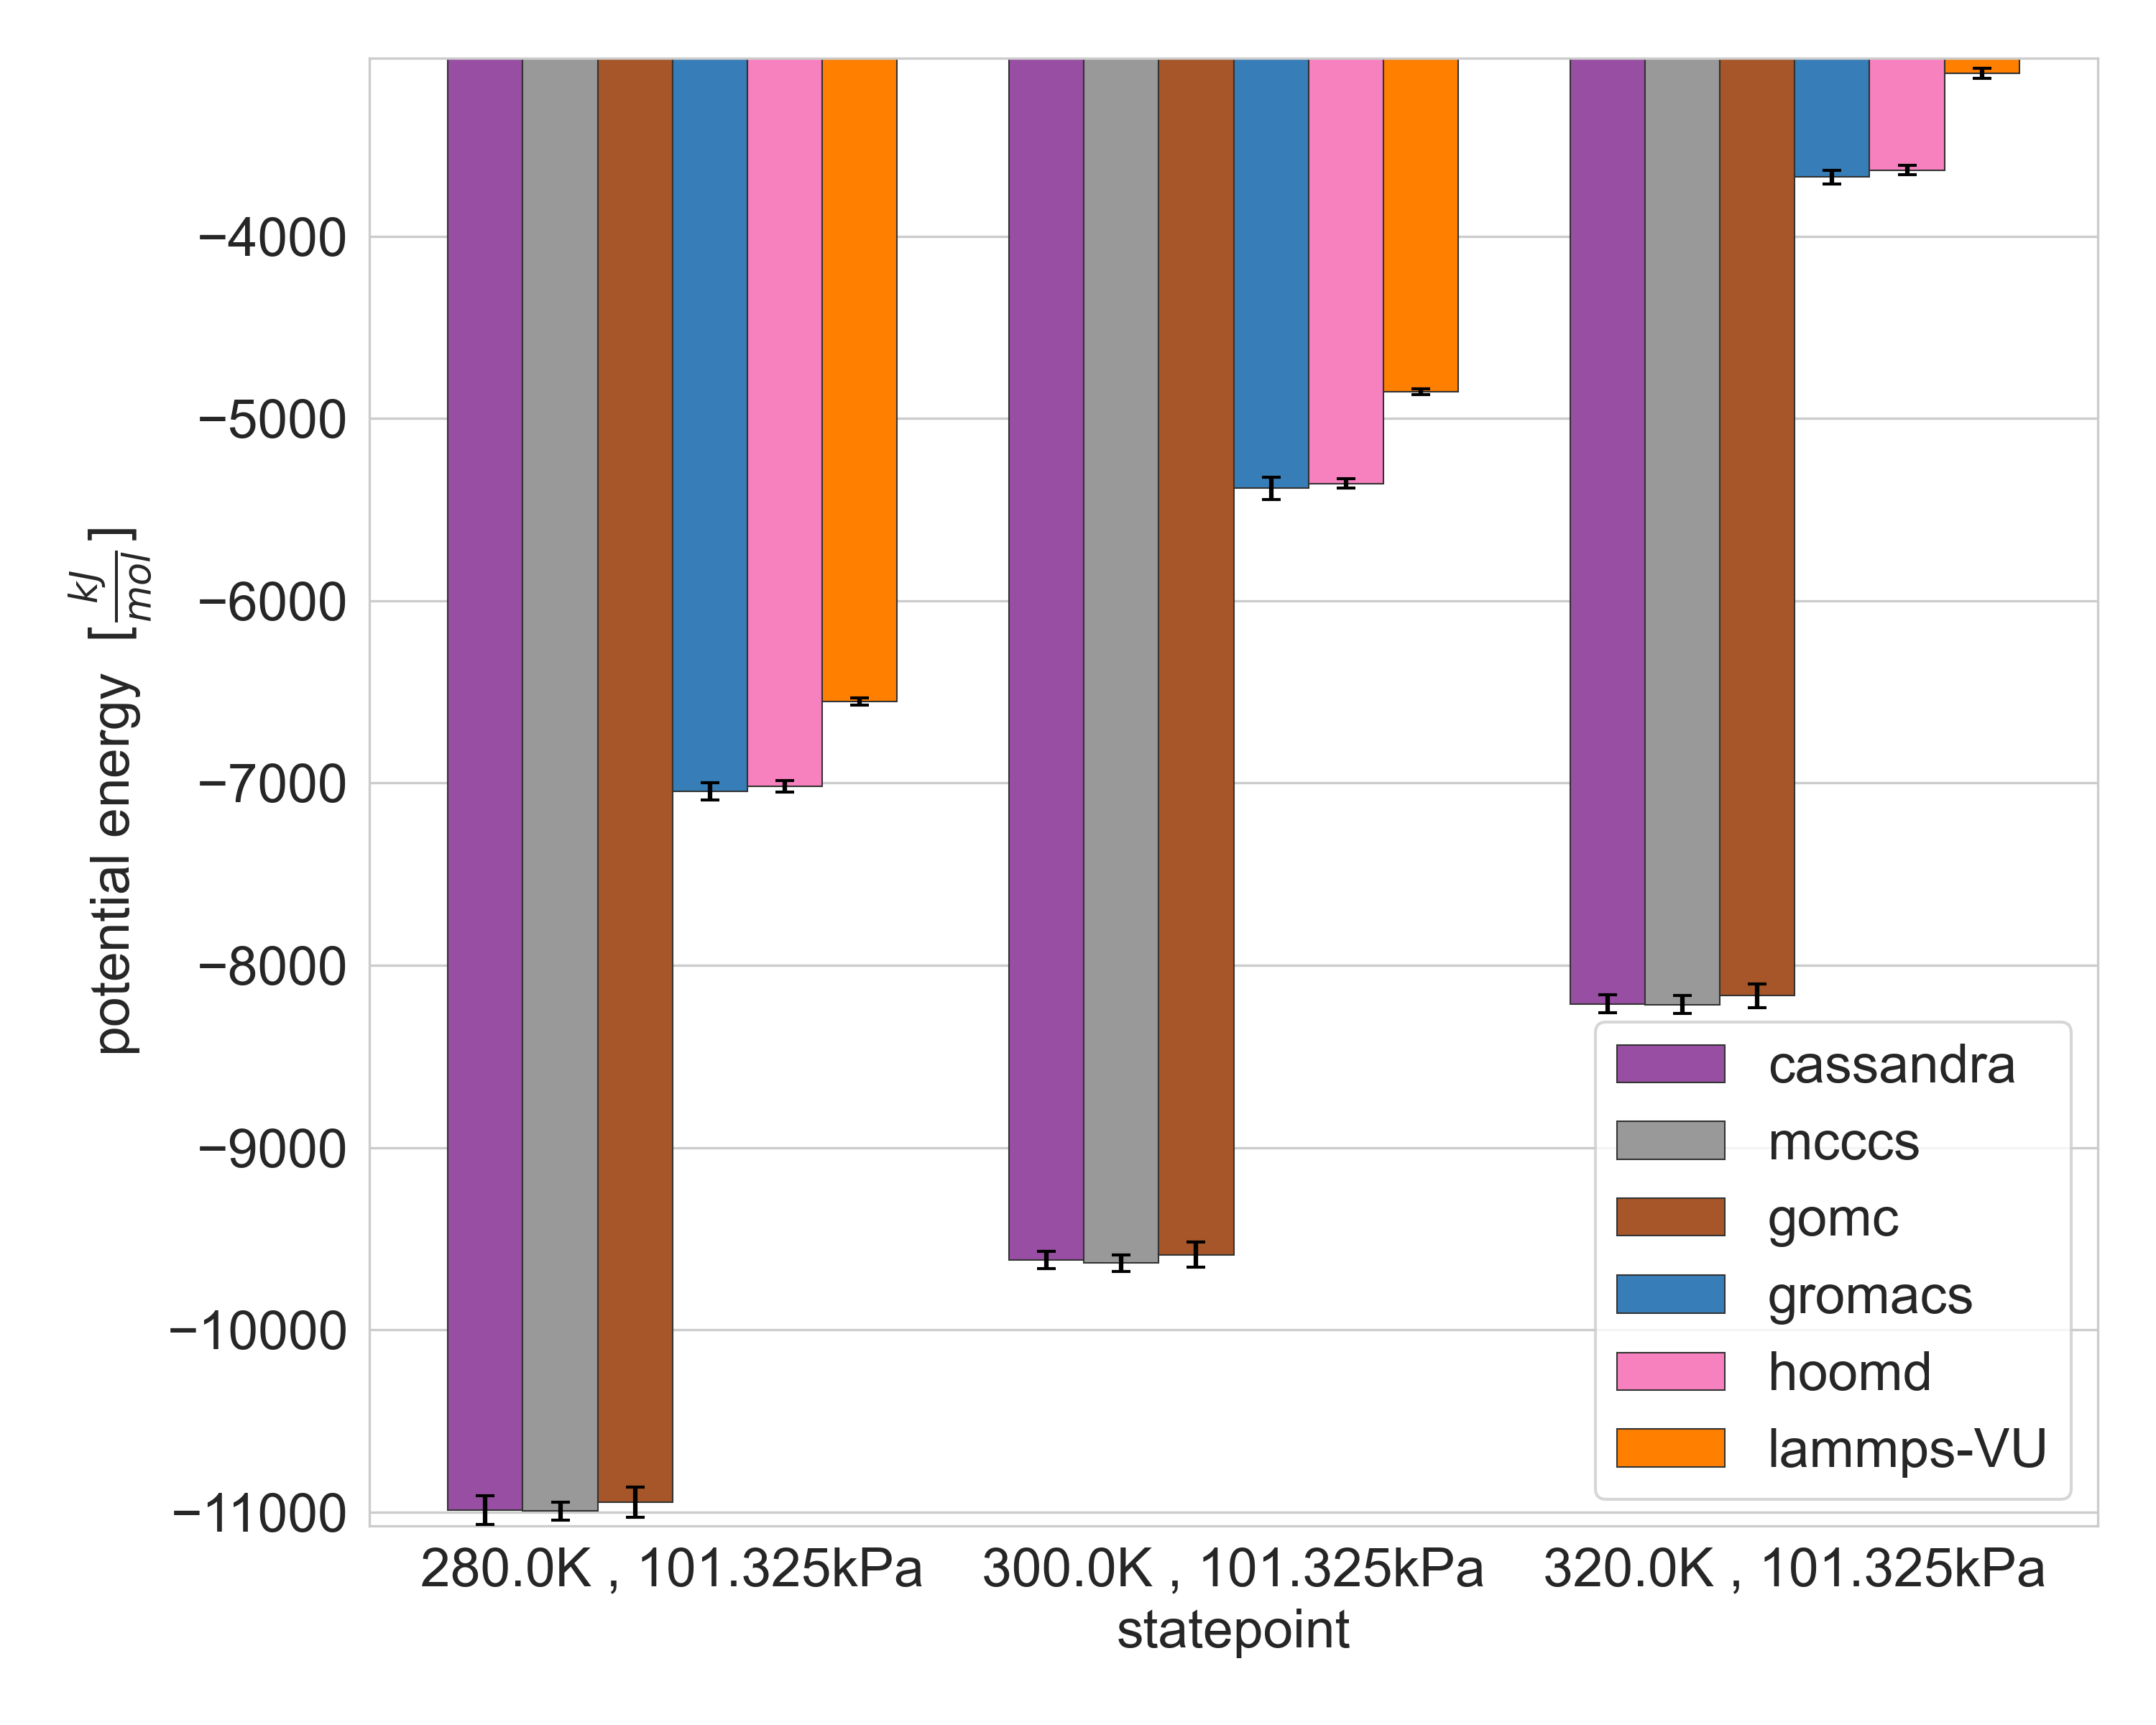
\includegraphics[width=0.6\linewidth,keepaspectratio]{figures/rep_study/ethanolAA_pe_summary.png}
    \caption{Average potential energy of ethanol by engine. The average is taken from independent samples of the equilibrated regions of 16 replicates. The error bars represent two standard deviations in each direction.}\label{fig:ethanol_pe}
\end{figure}
The first is that the MD engines are using flexible bonds while the MC engines are using fixed bonds.
\autoref{fig:pentane_pe} shows that when the only difference is whether bonds are flexible or fixed, the potential energy of the fixed bonds will be much lower, which explains the lower potential energy seen in the MC engines in \autoref{fig:ethanol_pe}.
The second is the yet to be understood discrepancy with LAMMPS in the PPPM model. 

\section{Conclusions}

Achieving equivalent results in molecular simulations can be tricky because it's not always possible to implement models identically in different engines.
For simple models like UA methane, sampling differences arise, but the engines largely agree.
As our models increase in complexity so do the deviations in our results between engines and methods.
There’s moderately good consensus among the UA pentane constrained-bond models, but the flexible bond model has greater variation and highlights the discrepancy when comparing against the constrained model.
The potential energy and density calculations of rigid UA benzene appear to demonstrate consensus, aside from MCCCS, but this deviation gives us a direction to investigate.
In the SPC/E water and AA ethanol simulations, we see much more variance between MD and MC engines but consistency among each simulation method.
Performing these consistency checks helps find bugs and identify modeling choices that give rise to these differences.

This study was a community-driven effort to show MoSDeF tools can help achieve reproducible results across engines.
Beyond just an opportunity to validate that our results were "correct", working on this project together with other simulators was an invaluable opportunity to learn.
Initially, this project seemed to be an easy task. 
However, it quickly became apparent that even seemingly minor choices relevant to the simulation parameters required discussion.
These discussions forced us to dig into each engines code in a way that helped us better understand the simulations we were running.
Each group brought a different background and expertise which was of great benefit when trying to pinpoint the source of a discrepancy.
Already, this collaboration has prompted many improvements to MoSDeF tools and the engines they support.
Ultimately the goal of molecular simulation is to probe the thermodynamic equilibrium of materials in ways which may give insight that experiment cannot.
In order to draw meaningful conclusions from simulation we must understand how the choices made in our model influence the results.